\newpage
\section{ỨNG DỤNG HÌNH HỌC CỦA TÍCH PHÂN}
\subsection{LÝ THUYẾT CẦN NHỚ}
\subsubsection{Tính diện tích hình phẳng}
\begin{khung4}{Ghi nhớ 1}
	\textbf{Hình phẳng giới hạn bởi một đồ thị hàm số, trục hoành và hai đường thẳng {\mathversion{bold}$x=a$, $x=b$}} \\
	\immini{
		Cho hàm số $y=f(x)$ liên tục trên đoạn $[a;b]$. Khi đó, diện tích hình phẳng giới hạn bởi đồ thị của hàm số $y=f(x)$, trục hoành và hai đường thẳng $x=a$, $x=b$ được tính bởi công thức
		$$S=\displaystyle\int\limits_{a}^{b}|f(x)|\mathrm{\,d}{x}.$$
	}
	{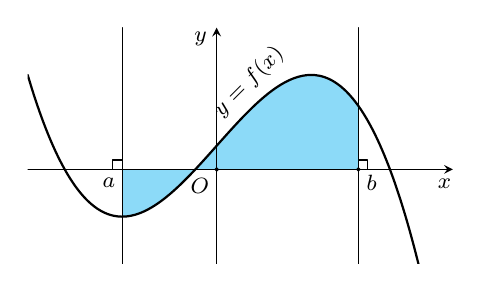
\begin{tikzpicture}[scale=0.6, line join=round, line cap=round, >=stealth, font=\footnotesize]
			\def\xmin{-4}
			\def\xmax{5}
			\def\ymin{-2}
			\def\ymax{3}
			%
			\clip (\xmin,\ymin) rectangle (\xmax,\ymax);
			\def\f{-3/32*(\x)^3+9/8*(\x)+1/2}
			\fill [cyan!90!white!50] {[domain=-2:3] plot (\x,{\f})} {[domain=3:-2] -- plot (\x,{0})} -- cycle;
			\draw [smooth, samples=100, thick] plot [domain=\xmin:\xmax] (\x, {\f})
			[samples at={1}] plot (\x, {\f}) node [above, rotate=45] {$y=f(x)$};
			\draw (-2,\ymin)--(-2,\ymax)
			(3,\ymin)--(3,\ymax);
			\draw [->] (\xmin,0)--(\xmax,0) node [below, xshift=-3pt] {$x$};
			\draw [->] (0,\ymin)--(0,\ymax) node [left, yshift=-4pt] {$y$};
			\draw [fill=black] (0,0) circle (1pt) ++(-135:.5) node {$O$}
			(-2,0) circle ++(-135:.4) node {$a$} 
			(3,0) circle (1pt) ++(-45:.4) node {$b$};
			\draw (-2,0) rectangle ++(-.2,.2) (3,0) rectangle ++(.2,.2);
	\end{tikzpicture}}
\end{khung4}
\begin{khung4}{Ghi nhớ 2}
	\textbf{Hình phẳng giới hạn bởi đồ thị của hai hàm số và hai đường thẳng {\mathversion{bold}$x=a$, $x=b$}} \\
	\immini{
		Cho hai hàm số $y=f_{1}(x)$, $y=f_{2}(x)$ liên tục trên đoạn $[a;b]$. Khi đó, diện tích hình phẳng giới hạn bởi hai đồ thị của hàm số $y=f_{1}(x)$, $y=f_{2}(x)$ và hai đường thẳng $x=a$, $x=b$ được tính bởi công thức
		$$S=\displaystyle\int\limits_{a}^{b}\left|f_{1}(x)-f_{2}(x) \right|\mathrm{\,d}{x}.$$
	}
	{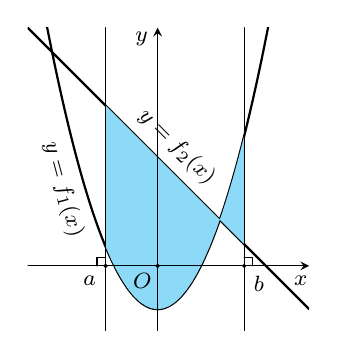
\begin{tikzpicture}[scale=0.55, line join=round, line cap=round, >=stealth, font=\footnotesize]
			\def\xmin{-3}
			\def\xmax{3.5}
			\def\ymin{-1.5}
			\def\ymax{5.5}
			\def\a{-1.2}
			\def\b{2}
			% Định nghĩa các hàm số
			\def\f{(\x)^2-1}
			\def\g{2.5-\x}
			\clip (\xmin,\ymin) rectangle (\xmax,\ymax);
			% Vẽ đồ thị các hàm số
			\draw[smooth, samples=100, thick] plot [domain=\xmin:\xmax] (\x, {\f})
			plot [domain=\xmin:\xmax] (\x, {\g})
			[samples at={-1.7}] plot (\x, {\f}) node [below, rotate=-75] {$y=f_{1}(x)$}
			[samples at={.1}] plot (\x, {\g}) node [above, rotate=-45] {$y=f_{2}(x)$}
			;
			% Tô vùng giữa hai đồ thị
			\fill [cyan!90!white!50] plot [domain=\a:\b] (\x, {\f}) -- plot[domain=\b:\a] (\x, {\g});
			%
			\draw [->] (\xmin,0)--(\xmax,0) node [below, xshift=-3pt] {$x$};
			\draw [->] (0,\ymin)--(0,\ymax) node [left, yshift=-4pt] {$y$};
			\draw [fill=black] (0,0) circle (1pt) ++(-135:.5) node {$O$};
			\draw (\a,\ymin)--(\a,\ymax)
			(\b,\ymin)--(\b,\ymax);
			\draw [fill=black] (\a,0) circle (1pt) node [below left] {$a$}
			(\b,0) circle (1pt) node [below right] {$b$};
			\draw (\a,0)++(-.2,0)--++(0,.2)--++(.2,0) (\b,0)++(.2,0)--++(0,.2)--++(-.2,0);
	\end{tikzpicture}}
\end{khung4}
%%%%%%%%%%%%%%%%%%%%%%%%%%%%%%%%%%
\subsubsection{Thể tích hình khối}
\begin{khung4}{Ghi nhớ 3}
	\textbf{Thể tích vật thể trong không gian} \\
	Trong không gian, cho một vật thể nằm trong khoảng không gian giữa hai mặt phẳng $(P)$ và $(Q)$ cùng vuông góc với trục $Ox$ tại các điểm $a$ và $b$. Mặt phẳng vuông góc với trục $Ox$ tại điểm có hoành độ $x$ $(a \le x \le b)$, cắt vật thể theo mặt cắt có diện tích $S(x)$. Khi đó, nếu $S(x)$ là hàm số liên tục trên đoạn $[a;b]$ thì thể tích vật thể được tính theo công thức 
	$$V=\displaystyle\int\limits_{a}^{b}{S(x)}\mathrm{\,d}{x}.$$
	\centerline{\begin{tikzpicture}[scale=0.4, >=stealth, line join=round, line cap=round,font=\footnotesize]
			\draw [thick, cyan!70!black!90]
			(0,0) coordinate (O) ++(4.44,1.67) coordinate (s11)
			.. controls +(.45,-.26) and +(-.56,.03) .. ++(1.72,-.53) coordinate (p11)
			.. controls +(.42,-.08) and +(-.63,-.4) .. ++(2.06,.58)
			(O) ++(10.19,2.25) .. controls +(.4,-.08) and +(-.37,.16) .. ++(1.24,-.23) coordinate (p21)
			.. controls +(.48,-.37) and +(-1.16,.11) .. ++(2.7,-.79)
			(O)  ++(15.5,1.24) .. controls +(.56,.16) and +(-.63,-.45) .. ++(1.88,.95) coordinate (p31)
			.. controls +(.5,.32) and +(.95,-1.06) .. ++(0,3.1) coordinate (p32)
			.. controls +(-.82,.69) and +(.79,-.13) .. ++(-1.69,-.03) coordinate (s32)
			(O) ++(14.13,5.56) .. controls +(-.53,-.03) and +(.93,.48) .. ++(-2.67,-1.03) coordinate (p22)
			.. controls +(-.24,-.05) and +(.5,-.08) .. ++(-1.24,0) coordinate (s22)
			(O) ++(8.23,5.21) .. controls +(-.71,.24) and +(1.24,.56) .. ++(-2.06,.63) coordinate (p12)
			.. controls +(-.5,-.21) and +(.56,.29) .. ++(-1.61,-.71) coordinate (s12)
			(O) ++(2.96,4.55) .. controls +(-.53,-.16) and +(-.4,.53) .. ++(-.29,-1.3)
			..controls +(-.16,-.45) and +(-.13,-.03) .. ++(.26,-.87)
			;
			\draw [dash pattern=on 1pt off 2pt, thick, cyan!70!black!90]
			(O) ++(8.23,1.72) .. controls +(.56,.26) and +(-.61,0) .. ++(1.96,.53) coordinate (s21)
			(O) ++(14.13,1.23) .. controls +(.37,-.05) and +(-.34,-.08) .. ++(1.38,.05) coordinate (s31)
			(O)  ++(15.69,5.27) .. controls +(-.37,.13) and +(.63,.05) .. ++(-1.56,.29)
			(O) ++(10.21,4.52) .. controls +(-.48,.13) and +(.93,-.05) .. ++(-1.98,.69)
			(O) ++(4.55,5.13) .. controls +(-.48,0) and +(.45,.32) .. ++(-1.59,-.58)
			(O) ++(2.94,2.38) .. controls +(.29,-.24) and +(-.61,.16) .. ++(1.51,-.71)
			;
			\fill [cyan!90!white!50] 
			(s11) 
			.. controls +(.58,.82) and +(1.27,-1.4) .. ++(.11,3.47)
			.. controls +(-.16,-.13) and +(0,.26) .. ++(-.34,-.66)
			.. controls +(-.34,-.21) .. ++(-.24,-.74)
			.. controls +(-.29,-.5) .. ++(.03,-.93)
			.. controls +(.03,-.29) .. ++(.24,-.45)
			.. controls +(-.2,-.48) .. ++(.21,-.69)
			(s21) 
			.. controls +(.77,-.08) and +(1.14,-.26) .. ++(.03,2.28)
			.. controls +(-.58,0) and +(-.87,.05) .. ++(-.03,-2.28)
			(s31) .. controls +(1.38,.69) and +(1.46,-.5) .. ++(.19,4.02)
			.. controls +(-.66,-.16) .. ++(-.66,-.82)
			.. controls +(-.19,-.29) .. ++(-.08,-.74)
			.. controls +(-.24,-.32) and +(-.4,.48) .. ++(.05,-1.38)
			.. controls +(-.08,-1.11) .. ++(.5,-1.08)
			;
			\draw [dash pattern=on 1pt off 2pt, cyan!70!black!90] 
			(s11) .. controls +(.58,.82) and +(1.27,-1.4) .. ++(.11,3.47)
			(s21) .. controls +(.77,-.08) and +(1.14,-.26) .. ++(.03,2.28)
			(s31) .. controls +(1.38,.69) and +(1.46,-.5) .. ++(.19,4.02)
			;
			\draw [thick, cyan!70!black!90] (s11)++(.11,3.47)
			.. controls +(-.16,-.13) and +(0,.26) .. ++(-.34,-.66)
			.. controls +(-.34,-.21) .. ++(-.24,-.74)
			.. controls +(-.29,-.5) .. ++(.03,-.93)
			.. controls +(.03,-.29) .. ++(.24,-.45)
			.. controls +(-.2,-.48) .. ++(.21,-.69)
			(s21)++(.03,2.28)
			.. controls +(-.58,0) and +(-.87,.05) .. ++(-.03,-2.28)
			(s31)++(.19,4.02)
			.. controls +(-.66,-.16) .. ++(-.66,-.82)
			.. controls +(-.19,-.29) .. ++(-.08,-.74)
			.. controls +(-.24,-.32) and +(-.4,.48) .. ++(.05,-1.38)
			.. controls +(-.08,-1.11) .. ++(.5,-1.08)
			;
			\newcommand{\p}[3]{
				\draw [thick] (#1)--(#1 |- 0,-.5)--++(-3.2,-2.5)--++(0,9.5)--++(3.2,2.5) node [below,pos=.5,sloped] {$#3$}--(#2);
			}
			\newcommand{\s}[1]{
				\draw [thick] (#1)--(#1 |- 0,0);
			}
			\newcommand{\my}[3]{
				\draw [dash pattern=on 1pt off 2pt] (#1 |- 0,0)--++(#2,0);
				\draw (#1 |- 0,0)++(#2,0)--(#3 |- 0,0);
			}
			\foreach \x/\y/\z in {11/12/x=a,21/22/,31/32/x=b}{
				\p{p\x}{p\y}{\z}
				\s{p\x}
				\draw [dash pattern=on 1pt off 2pt, thick] (p\x)--(p\y);
				\draw [thick] (s\x)--(s\x |- 0,0);
			}
			\foreach \x/\y/\z in {s11/-1.51/O,s21/-1.96/s11,s31/-1.38/s21}{
				\my{\x}{\y}{\z}
			}
			\draw [->] (s31 |- 0,0)--++(4,0) node [below] {$x$};
			\draw [->] (O)--++(0,8.5) node [left] {$z$};
			\draw [->] (O)--++(-3.2,-2.5) node [left] {$y$};
			\foreach \x/\y in {s11/a,s21/x,s31/b}{
				\draw [thick] (\x |- 0,0) node [below] {$\y$}++(.2,0)--++(0,.2)--++(-.2,0);
			}
			\draw ($(s21)!.5!(s22)$) node [xshift=1pt] {$S(x)$};
			\draw [fill=white] (O) circle (1pt) node [left] {$O$};
	\end{tikzpicture}}\\
\end{khung4}
\begin{khung4}{Ghi nhớ 4}
	\textbf{Thể tích khối tròn xoay} \\
	Cho $y=f(x)$ là hàm số liên tục và không âm trên đoạn $[a;b]$. Gọi $(D)$ là hình phẳng giới hạn bởi đồ thị hàm số $y=f(x)$, trục hoành và hai đường thẳng $x=a$, $x=b$. Quay $(D)$ quanh trục $Ox$ ta được một hình khối gọi là \textit{khối tròn xoay}. \\
	\centerline{
		\raisebox{-0.5\height}{
			\begin{tikzpicture}[scale=0.55,>=stealth,line join=round,line cap=round,font=\footnotesize]
				\def\xmin{-2}
				\def\xmax{9.5}
				\def\ymax{4}
				\def\ymax{5}
				\tikzset{declare function={
						f=-0.01*(\x)^3+0.14*(\x)^2-0.4*(\x)+2.2;}
				}
				\fill [pattern=dots] plot [domain=2:7] (\x,{f})--(7,0)--(2,0)--cycle;
				\draw [smooth, samples=100, thick] plot [domain=7:2] (\x,{f})
				[samples at={4.5}]  plot (\x,{f}) node [above, rotate=10] {$y=f(x)$}
				(2,0)--(2,\ymax) node [fill=white] {$x=a$}
				(7,0)--(7,\ymax) node [fill=white] {$x=b$};
				\draw [->] (0,0)--(\xmax,0) node [below, xshift=-3pt] {$x$};
				\draw [->] (0,0)--(0,\ymax) node [left, yshift=-4pt] {$y$};
				\draw [fill=black] 
				(0,0) circle (1pt) node [left] {$O$}
				(2,0) circle (1pt) node [below] {$a$}
				(7,0) circle (1pt) node [below] {$b$};
				\draw [->] (8,0.3) arc (135:-160:.2 and 0.5);
				\draw (4.5,1) node [fill=white, inner sep=1pt] {$(D)$};
			\end{tikzpicture}
		}
		\hspace*{.5cm}
		\raisebox{-0.5\height}{
			\begin{tikzpicture}[scale=0.55, line join=round, line cap=round, >=stealth, font=\footnotesize]
				\def\xmin{-2}
				\def\xmax{9.5}
				\def\ymax{4}
				\def\ymax{5}
				%
				\tikzset{declare function={
						f=-0.01*(\x)^3+0.14*(\x)^2-0.4*(\x)+2.2;
						g={-f};}
				}
				\draw [dash pattern=on 1pt off 2pt] (2,-1.88) arc (-90:90: 0.5 and 1.88);
				\draw [dash pattern=on 1pt off 2pt] (4,-2.2) arc (-90:90: 0.56 and 2.2);
				\fill [cyan!90!gray!80, opacity=.4] 
				(4,0) ellipse (0.56 and 2.2)
				(2,0) ellipse (0.5 and 1.88);
				\fill [pattern=dots, pattern color=gray] plot [domain=2:7] (\x,{f})--(7,0)--(2,0)--cycle;
				\draw (4,2.2) arc (90:270: 0.56 and 2.2);
				%
				\draw [samples at={5.4}]  plot (\x,{f}) node [above, rotate=10] {$y=f(x)$};
				%
				\draw [outer color=cyan!60, inner color=white, opacity=.4] plot [domain=7:2] (\x,{f})--(2,1.88) arc (90:270: 0.5 and 1.88)--plot [domain=2:7] (\x,{g}) arc (-90:-270:0.75 and 2.83);
				\draw [thick, fill=cyan!90!gray!80, opacity=.4] (7,0) ellipse (0.75 and 2.83);
				\draw [fill=black] 
				(0,0) circle (1pt) node [left] {$O$}
				(2,0) circle (1pt) node [below] {$a$}
				(7,0) circle (1pt) node [below] {$b$}
				(4,0) circle (1pt) node [below] {$x$}
				(0,2.2) circle (1pt) node [left] {$f(x)$};
				\draw (2,1.88)--(2,\ymax) node [fill=white] {$x=a$}
				(7,0)--(7,\ymax) node [fill=white] {$x=b$}
				(0,0)--(1.5,0);
				\draw [dash pattern=on 1pt off 2pt] (2,0)--(2,1.88)
				(4,0)--(4,2.2)--(0,2.2) 
				(1.5,0)--(7,0);
				\foreach \x in {2,4,7}{
					\draw (\x,0)++(0:.2)--++(90:.2)--++(180:.2);
				}
				%
				\draw [->] (4,-1)--(4,-3.5) node [below] {$S(x)=\pi f^{2}(x)$};
				\draw [->] (7,0)--(\xmax,0) node [below, xshift=-3pt] {$x$};
				\draw [->] (0,0)--(0,\ymax) node [left, yshift=-4pt] {$y$};
				\draw[->] (0,0)--(-2.5,-3) node [left] {$z$};
			\end{tikzpicture}
		}
	}\\
	Cắt khối tròn xoay trên bởi mặt phẳng vuông góc với trục $Ox$ tại điểm có hoành độ $x$ với $x \in [a; b]$, ta được mặt cắt là hình tròn có bán kính bằng $f(x)$ nên diện tích là $S(x)=\pi f^{2}(x)$. \\
	Vậy khối tròn xoay có thể tích là
	$$V=\pi\displaystyle\int\limits_{a}^{b}f^{2}(x)\mathrm{\,d}{x}.$$
	
\end{khung4}


%-------------------------------------------------------------------------------------------------------------
\subsection{PHÂN LOẠI VÀ PHƯƠNG PHÁP GIẢI TOÁN}
\begin{dang}{Xác định các đường giới hạn của hình phẳng}
	%	\begin{listEX}[1]
		%		\item [\ding{172}] Phương trình tổng quát của Parabol 
		%		\item [\ding{172}] 
		%	\end{listEX}
\end{dang}

\begin{vd}%[2D4N3-1]%[Dự án đề cương 3 khối NH24-25-Dot1-Trương Tường]
	\immini{
		Hình phẳng $(H)$ (phần tô đậm) ở hình bên được giới hạn bởi những đường nào?
	}
	{
		\begin{tikzpicture}[scale=0.6, >=stealth, line join=round]
			%% Định nghĩa khung
			\def\xmin{-1}
			\def\xmax{5}
			\def\ymin{-1}
			\def\ymax{3}
			%% Cắt hình
			\clip (\xmin,\ymin) rectangle (\xmax,\ymax);
			%% Định nghĩa các hàm số
			\def\f{2/(\x)}
			\def\g{0}
			%% Định nghĩa a và b
			\def\a{1}
			\def\b{4}
			%% Vẽ hệ trục
			\draw[->] (\xmin,0)--(\xmax,0) node [below, xshift=-3pt] {$x$};
			\draw[->] (0,\ymin)--(0,\ymax) node [left, yshift=-4pt] {$y$};
			\draw[fill=black] (0,0) circle (1pt) node [below left] {$O$};
			%% Vẽ đồ thị các hàm số
			\draw [smooth, samples=100, thick] plot [domain=.01:\xmax] (\x, {\f})
			[samples  at={2.5}] plot (\x, {\f}) node [above, rotate=-5] {$y=\dfrac{2}{x}$};
			%
			\fill [cyan!90!white!60] plot [domain=\a:\b] (\x, {\f}) -- plot[domain=\b:\a] (\x, {\g});
			%% Vẽ các đường thẳng x=a và x=b
			\draw (\a,\ymin)--(\a,\ymax)
			(\b,\ymin)--(\b,\ymax);
			%% Chú thích các điểm x=a và x=b
			\draw [fill=black] (\a,0) circle (1pt) node [below left] {$\a$}
			(\b,0) circle (1pt) node [below right] {$\b$}
			(2,.5) node [fill=white, inner sep=.5pt] {$(H)$};
		\end{tikzpicture}
	}
	\loigiai{
		Hình phẳng $(H)$ giới hạn bởi đồ thị hàm số $y=\dfrac{2}{x}$, trục hoành và hai đường thẳng $x=1$, $x=4$. 
	}
\end{vd}
\begin{vd}%[2D4H3-1]%[Dự án đề cương 3 khối NH24-25-Dot1-Trương Tường]
	\immini{
		Hình phẳng $(L)$ (phần tô đậm) ở hình bên được giới hạn bởi những đường nào?
	}
	{
		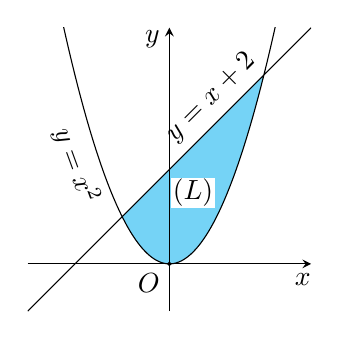
\begin{tikzpicture}[scale=.6, >=stealth, line join=round]
			%% Định nghĩa khung
			\def\xmin{-3}
			\def\xmax{3}
			\def\ymin{-1}
			\def\ymax{5}
			%% Định nghĩa các hàm số
			\def\f{(\x)^2}
			\def\g{(\x)+2}
			%% Định nghĩa a và b
			\def\a{-1}
			\def\b{2}
			\clip (\xmin,\ymin) rectangle (\xmax,\ymax);
			%% Vẽ đồ thị các hàm số
			\fill [cyan!90!white!60] plot [domain=\a:\b] (\x, {\f}) -- plot[domain=\b:\a] (\x, {\g});
			\draw[smooth, samples=100] plot [domain=\xmin:\xmax] (\x, {\f}) 
			plot [domain=\xmin:\xmax] (\x, {\g})
			[samples at={-1.5}] plot (\x, {\f}) node [below, rotate=-70] {$y=x^2$}
			[samples at={1.2}] plot (\x, {\g}) node [above, rotate=45] {$y=x+2$}
			(.5,1.5) node [fill=white, inner sep=.5pt] {$(L)$};
			%% Vẽ hệ trục
			\draw [->] (\xmin,0)--(\xmax,0) node [below, xshift=-3pt] {$x$};
			\draw [->] (0,\ymin)--(0,\ymax) node [left, yshift=-4pt] {$y$};
			\draw [fill=black] (0,0) circle (1pt) node [below left] {$O$};
		\end{tikzpicture}
	}
	\loigiai{
		Xét phương trình 
		\allowdisplaybreaks
		\begin{eqnarray*}
			& &x^2=x+2 \\
			& \Leftrightarrow & x^2-x-2=0 \\
			& \Leftrightarrow & \hoac{&x=-1\\&x=2.} 
		\end{eqnarray*}		
		Vậy hình phẳng $(L)$ giới hạn bởi đồ thị hai hàm số $y=x^2$, $y=x+2$ và hai đường  thẳng $x=-1$, $x=2$.
	}
\end{vd}
\begin{vd}%[2D4H3-2]%[Dự án đề cương 3 khối NH24-25-Dot1-Trương Tường]
	\immini{
		Mặt cắt của một đường hầm xuyên núi có dạng một parabol chiều cao $7{,}5$ m và rộng $12$ m. Chọn hệ trục tọa độ $Oxy$ sao cho $Oy$ là trục đối xứng của parabol và $Ox$ chứa  giao tuyến của mặt cắt và mặt đất như hình bên. Hỏi mặt cắt của hầm giới hạn bởi các đường nào?
	}
	{
		\begin{tikzpicture}[scale=0.25, >=stealth, line join=round]
			%% Định nghĩa khung
			\def\xmin{-7.5}
			\def\xmax{7.5}
			\def\ymin{0}
			\def\ymax{9}
			%% Định nghĩa các hàm số
			\def\f{-5/24*(\x)^2+7.5}
			\def\g{0}
			%% Định nghĩa a và b
			\def\a{-6}
			\def\b{6}
			%% Vẽ đồ thị các hàm số
			\draw [smooth, samples=100, thick] plot [domain=\a:\b] (\x, {\f});
			%
			\fill [pattern=dots] plot [domain=\a:\b] (\x, {\f}) -- plot[domain=\b:\a] (\x, {\g});
			%% Vẽ hệ trục
			\draw [->] (\xmin,0)--(\xmax,0) node [below, xshift=-3pt] {$x$};
			\draw [->] (0,\ymin)--(0,\ymax) node [left, yshift=-4pt] {$y$};
			\draw [fill=black] (0,0) circle (1pt) node [below] {$O$};
		\end{tikzpicture}
	}
	\loigiai{
		\immini{
			Vì parabol có đỉnh thuộc trục tung nên phương trình có dạng $y=ax^2+c$. \\
			Parabol đi qua hai điểm $(0;7{,}5)$ và $(6;0)$ nên ta có hệ phương trình \\
			$$\heva{&c= 7{,}5\\&36a+c= 0} 
			\Leftrightarrow 
			\heva{&a = -\dfrac{5}{24}\\&c = 7{,}5.}$$
			Do đó phương trình của parabol là $y=-\dfrac{5}{24}x^2+7{,}5$. \\
			Vậy mặt cắt của hầm giới hạn bởi đồ thị hàm số $y=-\dfrac{5}{24}x^2+7{,}5$, trục hoành và hai đường thẳng $x=-6$, $x=6$.
		}
		{
			\begin{tikzpicture}[scale=0.25, >=stealth, line join=round]
				%% Định nghĩa khung
				\def\xmin{-8}
				\def\xmax{8}
				\def\ymin{0}
				\def\ymax{11}
				%% Định nghĩa các hàm số
				\def\f{-5/24*(\x)^2+7.5}
				\def\g{0}
				%% Định nghĩa a và b
				\def\a{-6}
				\def\b{6}
				%% Vẽ đồ thị các hàm số
				\draw [smooth, samples=100, thick] plot [domain=\a:\b] (\x, {\f});
				%
				\fill [pattern=dots] plot [domain=\a:\b] (\x, {\f}) -- plot[domain=\b:\a] (\x, {\g});
				%% Vẽ hệ trục
				\draw [->] (\xmin,0)--(\xmax,0) node [below, xshift=-3pt] {$x$};
				\draw [->] (0,\ymin)--(0,\ymax) node [left, yshift=-4pt] {$y$};
				\draw [fill=black] (0,0) circle (1pt) node [below] {$O$}
				(-6,0) circle (1pt) node [below] {$-6$}
				(6,0) circle (1pt) node [below] {$6$}
				(0,7.5) circle (1pt) node [above left] {$7{,}5$};
			\end{tikzpicture}
		}
	}
\end{vd}
%%%%%%%%%%%%%%%%%%%%%%%%%%%%%%%%%%%%%%%%%%%%%%%
\begin{dang}{Tính diện tích hình phẳng}
	\begin{listEX}[1]
		\item [\ding{172}] Xác định các đường giới hạn của phần hình phẳng cần tính.
		\item [\ding{173}] Sử dụng công thức tính diện tích hình phẳng. 
	\end{listEX}
\end{dang}
\begin{vd}%[2D4H3-1]%[Dự án đề cương 3 khối NH24-25-Dot1-Trương Tường]
	Tính diện tích hình phẳng giới hạn bởi đồ thị hàm số $y=x^2-1$, trục hoành và hai đường thẳng $x=0$, $x=2$?
	\loigiai{
		Diện tích hình phẳng cần tính là $S=\displaystyle\int\limits_{0}^{2}\left|x^2-1\right|\mathrm{\,d}{x}$. \\
		Xét phương trình $x^2-1=0 \Leftrightarrow \hoac{&x = -1\\&x = 1.}$\\
		Do đó
		\allowdisplaybreaks 
		\begin{eqnarray*}
			S &=& \displaystyle\int\limits_{0}^{1}\left|x^2-1\right|\mathrm{\,d}{x}+\displaystyle\int\limits_{1}^{2}\left|x^2-1\right|\mathrm{\,d}{x}\\
			&=& \displaystyle\int\limits_{0}^{1}\left(1-x^2\right)\mathrm{\,d}{x}+\displaystyle\int\limits_{1}^{2}\left(x^2-1\right)\mathrm{\,d}{x} \quad (\text{vì  } x^2-1 \le 0, \; \forall  x \in [0;1] \text{ và } x^2-1 \ge 0, \; \forall  x \in [1;2]) \\
			&=&  \left.\left(x-\dfrac{x^3}{3}\right)\right|_{0}^{1}+\left.\left(\dfrac{x^3}{3}-x\right)\right|_{1}^{2} \\
			&=& \left(1-\dfrac{1}{3}\right)+\left(\dfrac{8}{3}-2\right)-\left(\dfrac{1}{3}-1\right) \\
			&=& 2.
		\end{eqnarray*}
	}
\end{vd}
\begin{vd}%[2D4H3-1]%[Dự án đề cương 3 khối NH24-25-Dot1-Trương Tường]
	\immini{
		Cho các đồ thị hàm số $y=\mathrm{e}^x$ và $y=2x-1$ có đồ thị như hình bên. Gọi $(H)$ là phần hình phẳng được tô đậm. 
		\begin{enumerate}
			\item Hình phẳng $(H)$ được giới hạn bởi các đường nào?
			\item Tính diện tích hình phẳng $(H)$? 
		\end{enumerate}
	}
	{
		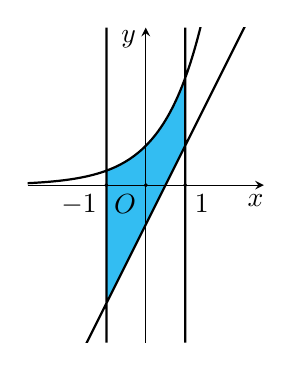
\begin{tikzpicture}[scale=0.5, >=stealth, line join=round]
			%% Định nghĩa khung
			\def\xmin{-3}
			\def\xmax{3}
			\def\ymin{-4}
			\def\ymax{4}
			%% Định nghĩa các hàm số
			\def\f{e^(\x)}
			\def\g{2*(\x)-1}
			%% Định nghĩa a và b
			\def\a{-1}
			\def\b{1}
			\clip (\xmin,\ymin) rectangle (\xmax,\ymax);
			%% Vẽ đồ thị các hàm số
			\fill [cyan!80] plot [domain=\a:\b] (\x, {\f}) -- plot[domain=\b:\a] (\x, {\g});
			\draw [smooth, samples=100, thick] plot [domain=\xmin:\xmax] (\x, {\f})
			plot [domain=\xmin:\xmax] (\x, {\g})
			(\a,\ymin)--(\a,\ymax) (\b,\ymin)--(\b,\ymax);
			%% Vẽ hệ trục
			\draw [->] (\xmin,0)--(\xmax,0) node [below, xshift=-3pt] {$x$};
			\draw [->] (0,\ymin)--(0,\ymax) node [left, yshift=-4pt] {$y$};
			\draw [fill=black] (0,0) circle (1pt) node [below left] {$O$}
			(\a,0) circle (1pt) node [below left] {$-1$}
			(\b,0) circle (1pt) node [below right] {$1$};
		\end{tikzpicture}
	}
	\loigiai{
		\begin{enumerate}
			\item Hình phẳng $(H)$ giới hạn bởi đồ thị hai hàm số $y=\mathrm{e}^x$, $y=2x-1$ và hai đường thẳng $x=-1$, $x=1$.
			\item Diện tích hình phẳng $(H)$ được tính theo công thức $S=\displaystyle\int\limits_{-1}^{1}\left|\mathrm{e}^x-(2x-1)\right|\mathrm{\,d}{x}$. \\
			Từ đồ thị ta có $\mathrm{e}^x>2x-1$ với mọi $x \in [-1;1]$. \\
			Do đó
			\allowdisplaybreaks
			\begin{eqnarray*}
				& S &= \displaystyle\int\limits_{-1}^{1}\left[\mathrm{e}^x-(2x-1)\right]\mathrm{d}{x} \\
				& &= \displaystyle\int\limits_{-1}^{1}\left(\mathrm{e}^x-2x+1\right)\mathrm{d}{x} \\
				& &= \left.\left(\mathrm{e}^x-x^2+x\right)\right|_{-1}^{1} \\
				& &= \left(\mathrm{e}-1+1\right)-\left(\mathrm{e}^{-1}-1-1\right) \\
				& &= \mathrm{e}-\dfrac{1}{\mathrm{e}}+2.
			\end{eqnarray*}
		\end{enumerate}
	}
\end{vd}
\begin{vd}%[2D4V3-2]%[Dự án đề cương 3 khối NH24-25-Dot1-Trương Tường]
	\immini{
		Mặt cắt của một đường hầm xuyên núi có dạng một parabol chiều cao $7{,5}$ m và rộng $12$ m. Chọn hệ trục tọa độ  $Oxy$ sao cho $Oy$ là trục đối xứng của parabol và $Ox$ chứa  giao tuyến của  mặt cắt và mặt đất như hình bên. Tính diện tích mặt cắt của đường hầm. 
	}
	{
		\begin{tikzpicture}[scale=0.25, >=stealth, line join=round]
			%% Định nghĩa khung
			\def\xmin{-7.5}
			\def\xmax{7.5}
			\def\ymin{0}
			\def\ymax{9}
			%% Định nghĩa các hàm số
			\def\f{-5/24*(\x)^2+7.5}
			\def\g{0}
			%% Định nghĩa a và b
			\def\a{-6}
			\def\b{6}
			%% Vẽ đồ thị các hàm số
			\draw [smooth, samples=100, thick] plot [domain=\a:\b] (\x, {\f});
			%
			\fill [pattern=dots] plot [domain=\a:\b] (\x, {\f}) -- plot[domain=\b:\a] (\x, {\g});
			%% Vẽ hệ trục
			\draw [->] (\xmin,0)--(\xmax,0) node [below, xshift=-3pt] {$x$};
			\draw [->] (0,\ymin)--(0,\ymax) node [left, yshift=-4pt] {$y$};
			\draw [fill=black] (0,0) circle (1pt) node [below] {$O$};
		\end{tikzpicture}
	}
	\loigiai{
		\immini{
			Vì parabol có đỉnh thuộc trục tung nên phương trình có dạng $y=ax^2+c$. \\
			Parabol đi qua hai điểm $(0;7{,5})$ và $(6;0)$ nên ta có  hệ phương trình \\
			$$\heva{&c= 7{,}5\\&36a+c= 0} 
			\Leftrightarrow 
			\heva{&a = -\dfrac{5}{24}\\&c = 7{,}5.}$$
			Do đó phương trình của parabol là $y=-\dfrac{5}{24}x^2+7{,}5$.
		}
		{
			\begin{tikzpicture}[scale=0.25, >=stealth, line join=round]
				%% Định nghĩa khung
				\def\xmin{-8}
				\def\xmax{8}
				\def\ymin{0}
				\def\ymax{11}
				%% Định nghĩa các hàm số
				\def\f{-5/24*(\x)^2+7.5}
				\def\g{0}
				%% Định nghĩa a và b
				\def\a{-6}
				\def\b{6}
				%% Vẽ đồ thị các hàm số
				\draw [smooth, samples=100, thick] plot [domain=\a:\b] (\x, {\f});
				%
				\fill [pattern=dots] plot [domain=\a:\b] (\x, {\f}) -- plot[domain=\b:\a] (\x, {\g});
				%% Vẽ hệ trục
				\draw [->] (\xmin,0)--(\xmax,0) node [below, xshift=-3pt] {$x$};
				\draw [->] (0,\ymin)--(0,\ymax) node [left, yshift=-4pt] {$y$};
				\draw [fill=black] (0,0) circle (1pt) node [below] {$O$}
				(-6,0) circle (1pt) node [below] {$-6$}
				(6,0) circle (1pt) node [below] {$6$}
				(0,7.5) circle (1pt) node [above left] {$7{,}5$};
			\end{tikzpicture}
		}
		\noindent
		Suy ra mặt cắt của hầm giới hạn bởi đồ thị hàm số  $y=-\dfrac{5}{24}x^2+7{,}5$, trục hoành và hai đường thẳng $x=-6$, $x=6$ nên có diện tích 
		\allowdisplaybreaks
		\begin{eqnarray*}
			& S &= \displaystyle\int\limits_{-6}^{6}\left|-\dfrac{5}{24}x^2+7{,}5\right|\mathrm{\,d}{x} \\
			& &= \displaystyle\int\limits_{-6}^{6}\left(-\dfrac{5}{24}x^2+7{,}5\right)\mathrm{\,d}{x} \quad \left(\text{vì }-\dfrac{5}{24}x^2+7{,}5 \ge 0, \forall x \in [-6;6]\right) \\
			& &= \left.\left(-\dfrac{5}{72}x^3+7{,}5x\right)\right|_{-6}^{6} \\
			& &= \left(-\dfrac{5}{72} \cdot 6^3 + 7{,}5\cdot 6\right)-\left[-\dfrac{5}{72} \cdot (-6)^3 + 7{,}5\cdot (-6)^3\right]\\
			& &= 60 \; \left(\text{m}^2\right).
		\end{eqnarray*}
	}
\end{vd}
%%%%%%%%%%%%%%%%%%%%
\begin{dang}{Tính thể tích vật thể trong không gian}
	\begin{listEX}[1]
		\item [\ding{172}] Chọn trục $Ox$ phù hợp. 
		\item [\ding{173}] Xác định vật thể nằm trong khoảng không gian giữa hai mặt phẳng $x=a$ và $x=b$ $(a<b)$.
		\item [\ding{174}] Tìm hàm số $S(x)$ biểu diễn diện tích mặt cắt vật thể tại điểm có hoành độ $x$ $(a \le x \le b)$. 
		\item [\ding{175}] Tính thể tích vật thể bằng công thức $V=\displaystyle\int\limits_{a}^{b}{S(x)}\mathrm{\,d}{x}.$
	\end{listEX}
\end{dang}
\begin{vd}%[2D4H3-4]%[Dự án đề cương 3 khối NH24-25-Dot1-Trương Tường]
	Trong không gian, cho một vật thể nằm giữa hai mặt phẳng vuông góc với trục hoành tại $x=1$ và $x=3$. Khi cắt vật thể bởi mặt phẳng vuông góc với $Ox$ tại điểm có hoành độ $x$ $(1 \le x \le 3)$ ta được thiết diện có diện tích $S(x)=4^x$. Tính thể tích của vật thể đã cho. 
	\loigiai{
		Thể tích của vật thể đã cho là
		$V = \displaystyle\int\limits_{1}^{3}S(x)\mathrm{\,d}{x}
		= \displaystyle\int\limits_{1}^{3}{4^x}\mathrm{\,d}{x}
		= \left.\dfrac{4^x}{\ln 4}\right|_{1}^{3} 
		= \dfrac{4^3}{\ln 4}-\dfrac{4^1}{\ln 4}
		= \dfrac{60}{\ln 4}$.
	} 
\end{vd}
\begin{vd}%[2D4H3-5]%[Dự án đề cương 3 khối NH24-25-Dot1-Trương Tường]
	\immini{
		Một bình chứa nước có hình dạng như hình bên. Biết rằng khi nước trong bình có chiều cao $x$ (dm) $\left(0 \le x \le 4\right)$ thì mặt nước là hình vuông có cạnh bằng $\sqrt{2+\dfrac{x^{2}}{4}}$ (dm). Thể tích của bình là bao nhiêu lít.
	}
	{
		\begin{tikzpicture}[scale=0.7,>=stealth,line join=round,line cap=round,font=\footnotesize]
			\path (0,0) coordinate (O)
			(.5,.5) coordinate (A)
			++(180:2) coordinate (B)
			++(45:1.5) coordinate (C)
			++($(A)-(B)$) coordinate (D)
			(A)++(.25,2.5) coordinate (A')
			(B)++(-.7,2.5) coordinate (B')
			(C)++(-.25,3) coordinate (C')
			(D)++(.7,3) coordinate (D')
			(A)++(.05,1.48) coordinate (A")
			(B)++(-.24,1.48) coordinate (B")
			(C)++(-.08,1.64) coordinate (C")
			(D)++(.24,1.64) coordinate (D")
			($(A)!.5!(C)$) coordinate (O)
			($(A')!.5!(C')$) coordinate (O')
			($(A")!.5!(C")$) coordinate (O")
			;
			\fill [cyan!90!white!50] (A) .. controls +(0,.32) and +(-.08,-.69) .. (A")--(B").. controls +(.16,-.45) and +(-.03,.63) .. (B)--cycle
			(A) .. controls +(0,.32) and +(-.08,-.69) .. (A")--(D") .. controls +(-.19,-.58) and +(.03,.5) .. (D)--cycle (A")--(B")--(C")--(D")--cycle;
			\draw (D)--(A)--(B) (A')--(B')--(C')--(D')--cycle (A")--(B")--(C")--(D")--cycle;
			\draw [dash pattern=on 1pt off 1.5pt] (B)--(C)--(D)
			(C) .. controls +(.03,.63) and +(.06,-.53) .. (C")
			(O)--(O') (O)--++(0:4) (O')--++(0:4) (O")--++(0:3)
			;
			\draw (A) .. controls +(0,.32) and +(-.08,-.69) .. (A") .. controls +(.03,.37) and +(-.11,-.26) .. (A')
			(B) .. controls +(-.03,.63) and +(.16,-.45) .. (B")
			.. controls +(-.08,.26) and +(.16,-.19) .. (B')
			(D) .. controls +(.03,.5) and +(-.19,-.58) .. (D")
			.. controls +(.13,.53) and +(-.16,-.32) .. (D')
			(C") .. controls +(-.05,.42) and +(.11,-.5) .. (C') 
			(O)++(0:.15)--++(90:.15)--++(180:.15)
			(O')++(0:.15)--++(-90:.15)--++(180:.15)
			(O")++(0:.15)--++(-90:.15)--++(180:.15)
			; 
			\draw [<->] (O)++(0:3.5)--++($(O')-(O)$) node [midway,right] {$4$ dm};
			\draw [<->] (O)++(0:2)--++($(O")-(O)$) node [midway,right] {$x$ dm};
			\draw [<-] ($(A")!.6!(B")$)--++(-150:1.5) node [left] {$\sqrt{2+\dfrac{x^{2}}{4}}$};
		\end{tikzpicture}
	}
	\loigiai{
		\immini{
			Chọn trục  $Ox$ chứa tâm của hai đáy bình như hình bên. \\
			Coi bình là vật thể nằm giữa hai mặt phẳng vuông góc với trục $Ox$ tại $x=0$ và $x=4$. \\
			Vì khi cắt bình bởi một mặt phẳng vuông góc với trục hoành tại điểm có hoành độ $x$ $(0 \le x \le 4)$ ta được thiết diện là hình vuông cạnh bằng $\sqrt{2+\dfrac{x^2}{4}}$ (dm). \\
			Diện tích của thiết diện là 
			$$S(x)=\left(\sqrt{2+\dfrac{x^2}{4}}\right)^2=2+\dfrac{x^2}{4} \; \left(\text{dm}^2\right).$$
		}
		{
			\begin{tikzpicture}[scale=0.7,>=stealth,line join=round,line cap=round,font=\footnotesize]
				\path (0,0) coordinate (O)
				(.5,.5) coordinate (A)
				++(180:2) coordinate (B)
				++(45:1.5) coordinate (C)
				++($(A)-(B)$) coordinate (D)
				(A)++(.25,2.5) coordinate (A')
				(B)++(-.7,2.5) coordinate (B')
				(C)++(-.25,3) coordinate (C')
				(D)++(.7,3) coordinate (D')
				(A)++(.05,1.48) coordinate (A")
				(B)++(-.24,1.48) coordinate (B")
				(C)++(-.08,1.64) coordinate (C")
				(D)++(.24,1.64) coordinate (D")
				($(A)!.5!(C)$) coordinate (O)
				($(A')!.5!(C')$) coordinate (O')
				($(A")!.5!(C")$) coordinate (O")
				;
				\fill [cyan!90!white!50] (A) .. controls +(0,.32) and +(-.08,-.69) .. (A")--(B").. controls +(.16,-.45) and +(-.03,.63) .. (B)--cycle
				(A) .. controls +(0,.32) and +(-.08,-.69) .. (A")--(D") .. controls +(-.19,-.58) and +(.03,.5) .. (D)--cycle (A")--(B")--(C")--(D")--cycle;
				\draw (D)--(A)--(B) (A')--(B')--(C')--(D')--cycle (A")--(B")--(C")--(D")--cycle;
				\draw [dash pattern=on 1pt off 1.5pt] (B)--(C)--(D)
				(C) .. controls +(.03,.63) and +(.06,-.53) .. (C")
				(O)--(O') (O)--++(0:4) (O')--++(0:4) (O")--++(0:3)
				;
				\draw (A) .. controls +(0,.32) and +(-.08,-.69) .. (A") .. controls +(.03,.37) and +(-.11,-.26) .. (A')
				(B) .. controls +(-.03,.63) and +(.16,-.45) .. (B")
				.. controls +(-.08,.26) and +(.16,-.19) .. (B')
				(D) .. controls +(.03,.5) and +(-.19,-.58) .. (D")
				.. controls +(.13,.53) and +(-.16,-.32) .. (D')
				(C") .. controls +(-.05,.42) and +(.11,-.5) .. (C') 
				(O)++(0:.15)--++(90:.15)--++(180:.15)
				(O')++(0:.15)--++(-90:.15)--++(180:.15)
				(O")++(0:.15)--++(-90:.15)--++(180:.15)
				; 
				\draw [<->] (O)++(0:3.5)--++($(O')-(O)$) node [midway,right] {$4$ dm};
				\draw [<->] (O)++(0:2)--++($(O")-(O)$) node [midway,right] {$x$ dm};
				\draw [<-] ($(A")!.6!(B")$)--++(-150:1.5) node [left] {$\sqrt{2+\dfrac{x^{2}}{4}}$};
				\draw (O) circle (1pt)+(-90:.3) node {$O$}
				(O')  circle (1pt) +(180:.4) node {$4$};
				\draw [->] (O')--++(90:1.5) node [left, yshift=-3pt] {$x$};
			\end{tikzpicture}
		}
		\noindent
		Thể tích của bình nước là 
		$$V=\displaystyle\int\limits_{0}^{4}S(x)\mathrm{\,d}{x}
		=\displaystyle\int\limits_{0}^{4}\left(2+\dfrac{x^2}{4}\right)\mathrm{\,d}{x}
		=\left.\left(2x+\dfrac{x^3}{12}\right)\right|_{0}^{4} 
		=2 \cdot 4 +\dfrac{4^3}{12}
		=\dfrac{40}{3} \; \left(\text{dm}^3\right).$$
		Vậy thể tích của bình là $\dfrac{40}{3}$ lít.
	}
\end{vd}
\begin{vd}%[2D4V3-4]%[Dự án đề cương 3 khối NH24-25-Dot1-Trương Tường]
	\immini{
		Cho khối chóp tứ giác đều có cạnh đáy bằng $a$ và chiều cao bằng $h$. Chọn mặt phẳng tọa độ $Oxy$ sao cho $O$ trùng với đỉnh khối chóp và tia $Ox$ chứa chiều cao của hình chóp. Cắt khối chóp bởi mặt phẳng cách đỉnh $O$ một khoảng bằng $x$ $(0  \le x \le h)$ ta được thiết diện là hình vuông $(L)$ có diện tích $S(x)$ (như hình bên).
		\begin{enumerate}
			\item Tính độ dài đường chéo của hình vuông $(L)$ theo $a$, $h$ và $x$. 
			\item Tính diện tích $S(x)$ theo $a$, $h$ và $x$.
			\item Tính thể tích khối chóp đã cho theo $a$ và $h$. 
		\end{enumerate}
	}
	{
		\begin{tikzpicture}[scale=0.5,>=stealth,line join=round,line cap=round,font=\footnotesize]
			\path
			(0,0) coordinate (D)
			++(5,0) coordinate (C)
			++(-2,-2) coordinate (B)
			++($(D)-(C)$) coordinate (A)
			($(A)!.5!(C)$) coordinate (H) coordinate (h)
			($(H)+(90:5)$) coordinate (O)
			\foreach \x in {A,B,C,D}{
				($(O)!.45!(\x)$) coordinate (\x')
			}
			($(A')!.5!(C')$) coordinate (H') coordinate (x)
			;
			\fill [cyan!90!white!50] (A')--(B')--(C')--(D')--cycle (A)--(B)--(C)--(D)--cycle;
			\draw [dash pattern=on 1pt off 2pt] (A)--(D)--(C) (O)--(H) (A')--(C') (O)--(D) (A)--(C) (A')--(D')--(C')
			;
			\draw [semithick] (A)--(B)--(C) (B)--(O) (A)--(O) (C)--(O) (A')--(B')--(C')
			;
			\foreach \x/\y in {A,B,C,D,H,H',A',B',C',D'}{
				\draw [fill=black] (\x) circle (1pt);
			}
			\draw [->, dashed] (H)--++(-90:.8) node [left, yshift=2pt] {$x$};
			\pic [draw, angle radius=0.1cm] {right angle=C--H--O};
			\pic [draw, angle radius=0.1cm] {right angle=C'--H'--O};
			\draw (O) circle (1pt) +(90:.4) node {$O$}
			(x) circle (1pt) ++(-30:.4) node {$x$}
			(h) circle (1pt) ++(-30:.4) node {$h$};
		\end{tikzpicture}
	}
	\loigiai{
		\immini{
			\begin{enumerate}
				\item Gọi $ABCD$ là đáy của hình chóp; $A'$, $C'$ là giao điểm của mặt cắt và hai cạnh $OA$, $OC$; $H$ và $H'$ theo thứ tự là tâm của hình vuông $ABCD$ và hình vuông $(L)$. \\
				Theo đề bài, ta có $OH=h$; $OH'=x$; $AH=\dfrac{AC}{2}=\dfrac{a\sqrt{2}}{2}$. \\
				Tam giác $OAH$ có $A'H' \parallel AH$ nên 
				$$\dfrac{A'H'}{AH}=\dfrac{OH'}{OH} \quad \text{hay} \quad \dfrac{A'H'}{\dfrac{a\sqrt{2}}{2}}=\dfrac{x}{h} \Leftrightarrow A'H'=\dfrac{ax\sqrt{2}}{2h}.$$ 
				Độ dài đường chéo hình vuông $(L)$ là $A'C'=2\cdot A'H'=\dfrac{ax\sqrt{2}}{h}$.
			\end{enumerate}
		}
		{
			\begin{tikzpicture}[scale=0.5,>=stealth,line join=round,line cap=round,font=\footnotesize]
				\path
				(0,0) coordinate (D)
				++(5,0) coordinate (C)
				++(-2,-2) coordinate (B)
				++($(D)-(C)$) coordinate (A)
				($(A)!.5!(C)$) coordinate (H) coordinate (h)
				($(H)+(90:5)$) coordinate (O) coordinate (O)
				\foreach \x in {A,B,C,D}{
					($(O)!.45!(\x)$) coordinate (\x')
				}
				($(A')!.5!(C')$) coordinate (H') coordinate (x)
				;
				\fill [cyan!90!white!50] (A')--(B')--(C')--(D')--cycle;
				\draw [dash pattern=on 1pt off 2pt] (A)--(D)--(C) (O)--(H) (A')--(C') (O)--(D) (A)--(C) (A')--(D')--(C')
				;
				\draw [semithick] (A)--(B)--(C) (B)--(O) (A)--(O) (C)--(O) (A')--(B')--(C')
				;
				\foreach \x/\y in {A/-90,B/-90,C/0,D/170,H/150,A'/180,C'/10,H'/150,O/90,h/-45,x/-30}{
					\draw [fill=black] (\x) circle (1pt) ++(\y:0.4) node {$\x$};
				}
				\draw [->, dash pattern=on 1pt off 2pt] (H)--++(-90:.8) node [left] {$x$};
				\pic [draw, angle radius=0.1cm] {right angle=C--H--O};
				\pic [draw, angle radius=0.1cm] {right angle=C'--H'--O};
			\end{tikzpicture}
		}
		\begin{enumerate}
			\setcounter{enumi}{1}
			\item Độ dài cạnh hình vuông $(L)$ là $\dfrac{A'H'}{\sqrt{2}}=\dfrac{ax}{h}$. \\
			Diện tích hình vuông $(L)$ là 
			$$S(x)=\left(\dfrac{ax}{h}\right)^2=\dfrac{a^2x^2}{h^2}.$$
			\item Coi khối chóp đã cho là vật thể nằm  giữa hai mặt phẳng vuông góc với $Ox$ tại điểm $x=0$, $x=h$. Khi cắt khối chóp bởi mặt phẳng vuông góc với $Ox$ tại điểm có hoành độ $x$ $(0 \le x \le h)$ ta được thiết diện có diện tích $S(x)$ nên khối chóp có thể tích là 
			$$V=\displaystyle\int\limits_{0}^{h}S(x)\mathrm{\,d}{x}
			=\displaystyle\int\limits_{0}^{h}\dfrac{a^2x^2}{h^2}\mathrm{\,d}{x}
			=\left.\left(\dfrac{a^2x^3}{3h^2}\right)\right|_{0}^{h} 
			=\dfrac{a^2 \cdot h^3}{3h^2}
			=\dfrac{1}{3}a^2h.$$
		\end{enumerate}
	}
\end{vd}
%%%%%%%%%%%%%%%%%%%%%%%%%%%%%%%%%%%%%%
\begin{dang}{Tính thể tích khối tròn xoay}
	\begin{listEX}[1]
		\item[\ding{172}] Xác định phần hình phẳng quay quanh trục $Ox$.
		\item[\ding{173}] Sử dụng công thức tính thể tích khối tròn xoay. 
	\end{listEX}
\end{dang}
\begin{vd}%[2D4N3-3]%[Dự án đề cương 3 khối NH24-25-Dot1-Trương Tường]
	Gọi $(H)$ là phần hình phẳng giới hạn bởi đồ thị hàm số $y=2\sqrt{x}$, trục hoành và hai đường thẳng $x=0$, $x=4$. Tính thể tích khối tròn xoay được tạo thành khi quay hình phẳng $(H)$ quay trục hoành?
	\loigiai{
		Thể tích khối tròn xoay cần tìm là 
		$V=\pi\displaystyle\int\limits_{0}^{4}\left(2\sqrt{x}\right)^2\mathrm{\,d}{x}
		=\pi\displaystyle\int\limits_{0}^{4}{4x}\mathrm{\,d}{x}
		=\pi\left.\left(2x^2\right)\right|_{0}^{4}
		=32\pi$.
	}
\end{vd}
\begin{vd}%[2D4V3-3]%[Dự án đề cương 3 khối NH24-25-Dot1-Trương Tường]
	\immini{
		Trong mặt phẳng tọa độ $Oxy$, cho hình thang $OABC$ với $A(0;1)$, $B(3;2)$ và $C(3;0)$ như hình bên. 
		\begin{enumerate}
			\item Hình thang $OABC$ được giới hạn bởi những đường có phương trình nào?
			\item Tính thể tích khối tròn xoay được tạo thành khi quay hình thang $OABC$ quanh trụch hoành.
		\end{enumerate}
	}
	{
		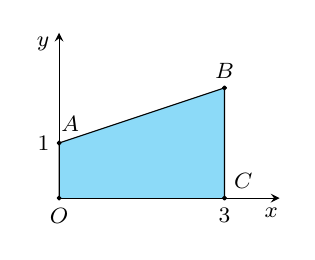
\begin{tikzpicture}[scale=0.7,>=stealth,line join=round,line cap=round,font=\footnotesize]
			\def\xmin{0} 
			\def\xmax{4}
			\def\ymin{0} 
			\def\ymax{3} 
			\draw [fill=cyan!90!white!50] (0,0)--(0,1)--(3,2)--(3,0);
			\draw [->] (\xmin,0)--(\xmax,0) node [below, xshift=-3pt] {$x$};
			\draw [->] (0,\ymin)--(0,\ymax) node [left, yshift=-4pt] {$y$};
			\draw [fill=black] (0,0) circle (1pt) node [below] {$O$}
			(0,1) circle (1pt) node [left] {$1$}
			(3,2) circle (1pt) node [above] {$B$}
			(3,0) circle (1pt) node [below] {$3$}
			(3,0) node [above right] {$C$}
			(0,1)++(60:.4) node {$A$};			
		\end{tikzpicture}
	}
	\loigiai{
		\begin{enumerate}
			\immini{
				\item Phương trình đường thẳng $AB$ có dạng $y=ax+b$. \\
				Đường thẳng $AB$ đi qua hai điểm $A(0;1)$ và $B(3;2)$ nên ta có hệ phương trình
				$$\heva{&b = 1\\&3a+b = 2}
				\Leftrightarrow
				\heva{&a = \dfrac{1}{3}\\&b = 1.}$$ 
				Do đó $AB\colon y=\dfrac{1}{3}x+1$.
			}
			{
				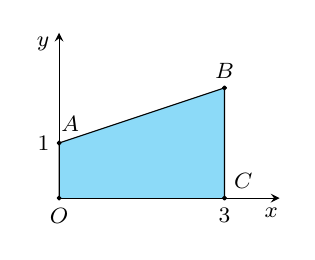
\begin{tikzpicture}[scale=0.7,>=stealth,line join=round,line cap=round,font=\footnotesize]
					\def\xmin{0} 
					\def\xmax{4}
					\def\ymin{0} 
					\def\ymax{3} 
					\draw [fill=cyan!90!white!50] (0,0)--(0,1)--(3,2)--(3,0);
					\draw [->] (\xmin,0)--(\xmax,0) node [below, xshift=-3pt] {$x$};
					\draw [->] (0,\ymin)--(0,\ymax) node [left, yshift=-4pt] {$y$};
					\draw [fill=black] (0,0) circle (1pt) node [below] {$O$}
					(0,1) circle (1pt) node [left] {$1$}
					(3,2) circle (1pt) node [above] {$B$}
					(3,0) circle (1pt) node [below] {$3$}
					(3,0) node [above right] {$C$}
					(0,1)++(60:.4) node {$A$};			
				\end{tikzpicture}
			}
			Vậy hình thang $OABC$ được giới hạn bởi đồ thị hàm số $y=\dfrac{1}{3}x+1$, trục hoành và hai đường thẳng $x=0$, $x=3$. 
			\item Thể tích khối tròn xoay được tạo thành là
			$$V=\pi \displaystyle\int\limits_{0}^{3}\left(\dfrac{1}{3}x+1\right)^2\mathrm{\,d}{x}
			=\pi\displaystyle\int\limits_{0}^{3}\left(\dfrac{1}{9}x^2+\dfrac{2}{3}x+1\right)\mathrm{\,d}{x}
			=\pi\left(\dfrac{x^3}{27}+\dfrac{x^2}{3}+x\right)\Bigg|_{0}^{3}
			=\pi\left(\dfrac{3^3}{27}+\dfrac{3^2}{3}+3\right)
			=7\pi.$$
		\end{enumerate}
	}
\end{vd}

\begin{vd}%[2D4V3-3]%[Dự án đề cương 3 khối NH24-25-Dot1-Trương Tường]
	Cho khối cầu có bán kính $R$. Cắt khối cầu bởi một mặt phẳng ta được khối chỏm cầu bán kính $R$, chiều cao $h$. Chọn mặt phẳng tọa độ $Oxy$ sao cho gốc $O$ trùng với tâm mặt cầu, $Ox$ vuông góc với mặt cắt (tham  khảo hình bên dưới). \\
	\begin{minipage}{.33\textwidth}
		\centering
		\begin{tikzpicture}[scale=0.5,>=stealth,line join=round,line cap=round,font=\footnotesize]
			\path 
			(0,0) coordinate (O)
			(2,{2*sqrt(3)}) coordinate (A)
			(2,{-2*sqrt(3)}) coordinate (B);
			\draw [ball color=gray!5] (0,0) circle (4);
			\fill [ball color=cyan!70] (A) arc (60:-60:{4}) arc (-90:90:{.75} and {2*sqrt(3)})--cycle;
			\fill [pattern=north east lines] (2,0) ellipse ({.75} and {2*sqrt(3)});
			\draw (2,{2*sqrt(3)}) arc (90:-90:{.75} and {2*sqrt(3)}) (0,4) arc (90:-90:{sqrt(3)/2} and {4});
			\draw [dash pattern=on 1pt off 1.5pt] (2,{2*sqrt(3)}) arc (90:270:{.75} and {2*sqrt(3)}) (2,0)--(2,{2*sqrt(3)}) (0,4) arc (90:270:{sqrt(3)/2} and {4}) (0,0)--(4,0)
			(4,0)--(4,4) (O)--++(90:4);
			\draw [<->] (2,{2*sqrt(3)})--++(0:2) node [midway,fill=white,inner sep=0pt] {$h$};
			\draw [<->] (0,4)--(4,4) node [midway,fill=white,inner sep=0pt] {$R$};
			\fill (0,0) circle (1pt) (2,0) circle (1pt);
		\end{tikzpicture}
	\end{minipage}
	\begin{minipage}{.33\textwidth}
		\centering
		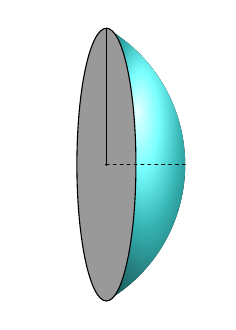
\begin{tikzpicture}[scale=0.5,>=stealth,line join=round,line cap=round,font=\footnotesize]
			\path 
			(0,0) coordinate (O)
			(2,{2*sqrt(3)}) coordinate (A)
			(2,{-2*sqrt(3)}) coordinate (B);
			\fill [ball color=cyan!70] (A) arc (60:-60:{4}) arc (-90:90:{.75} and {2*sqrt(3)})--cycle;
			\draw [fill=gray!80] (2,0) ellipse ({.75} and {2*sqrt(3)});
			\draw [dash pattern=on 1pt off 1.5pt] (2,0)--(4,0);
			\draw (2,0)--(2,{2*sqrt(3)});
			\fill (2,0) circle (1pt);
		\end{tikzpicture}
	\end{minipage}
	\begin{minipage}{.33\textwidth}
		\centering
		\begin{tikzpicture}[scale=0.5,>=stealth,line join=round,line cap=round,font=\footnotesize]
			\def\xmax{5.5}
			\def\ymin{-5.5} 
			\def\ymax{5.5} 
			\def\zmax{4}
			\fill [cyan!100!black!40] (0,0)++(4,0) arc (0:60:{4})--(2,0)--cycle;
			\draw (0,0) ellipse ({sqrt(3)/2} and {4});
			\draw (0,4) arc (90:-90:{4}) (2,{2*sqrt(3)}) arc (90:-90:{.75} and {2*sqrt(3)});
			\draw [dash pattern=on 1pt off 1.5pt] (2,{2*sqrt(3)}) arc (90:270:{.75} and {2*sqrt(3)}) (2,0)--(2,{2*sqrt(3)}) (O)--(4,0);
			\draw [->] (4,0)--(\xmax,0) node [below, xshift=-3pt] {$x$};
			\draw [->] (0,\ymin)--(0,\ymax) node [left, yshift=-4pt] {$y$};
			\draw [->] (0,0)--++(-135:\zmax) node [above] {$z$};
			\fill [black] (0,0) circle (1pt) node [left] {$O$}
			(2,0) circle (1pt) node [below] {$R-h$}
			(4,0) circle (1pt) node [below right] {$R$};
		\end{tikzpicture}
	\end{minipage}
	\begin{enumerate}
		\item Khối chỏm cầu được tạo thành khi quay quanh trục hoành phần hình phẳng giới hạn bởi những đường nào?
		\item Tính thể tích khối chỏm cầu theo $R$ và $h$.
	\end{enumerate}
	\loigiai{
		\begin{enumerate}
			\item Mặt phẳng $(Oxy)$ cắt khối cầu theo một đường tròn tâm $O$, bán kính $R$ nên có phương trình 
			$$x^2+y^2=R^2.$$
			Do đó, nửa đường tròn nằm phía trên trục hoành là đồ thị hàm số có phương trình $$y=\sqrt{R^2-x^2}.$$
			Vậy khối chỏm cầu được tạo thành khi quay quanh trục hoành phần hình phẳng giới hạn bởi đồ thị hàm số $y=\sqrt{R^2-x^2}$, trục hoành và hai đườngthẳng $x=R-h$, $x=R$.
			\item Thể tích khối chỏm cầu được tính theo công thức
			\allowdisplaybreaks
			\begin{eqnarray*}
				&V&= \pi\displaystyle\int\limits_{R-h}^{R}\left(\sqrt{R^2-x^2}\right)^2\mathrm{\,d}{x} \\
				&&= \pi\displaystyle\int\limits_{R-h}^{R}\left(R^2-x^2\right)\mathrm{\,d}{x} \\
				&&= \pi\left(R^2x - \dfrac{x^3}{3}\right)\Bigg|_{R-h}^{R} \\
				&&= \pi \left[R^3-\dfrac{R^3}{3}-R^2 \cdot (R-h)+\dfrac{(R-h)^3}{3}\right] \\
				&&= \pi \left(R^3 - \dfrac{R^3}{3}-R^3+R^2h+\dfrac{R^3-3R^2h+3Rh^2-h^3}{3}\right) \\
				&&= \pi\left(Rh^2-\dfrac{h^3}{3}\right) \\
				&&= \pi h^2\left(R-\dfrac{h}{3}\right).
			\end{eqnarray*}
		\end{enumerate}
	}
\end{vd}
%-----------------------------------------------------------------------------
\subsection{Bài tập rèn luyện}
\ind{PHẦN I.} \inden{Câu trắc nghiệm nhiều phương án lựa chọn. Mỗi câu hỏi học sinh chỉ chọn một phương án.}\\
\setcounter{ex}{0}
\Opensolutionfile{ans}[ans/2D4-Bai3-TN]%
%----Mức độ Nhận biết-----%
\begin{ex}%[2D4N3-1]%[Dự án đề cương 3 khối NH24-25-Dot1-Trương Tường]
	Công thức nào sau đây tính diện tích $S$ của hình phẳng giới hạn bởi đồ thị hàm số $y=x^3$, trục hoành và hai đường thẳng $x=-1$, $x=2$?
	\choice
	{$S=-\displaystyle\int\limits_{-1}^{2}{\dfrac{x^{4}}{4}}\mathrm{\,d}{x}$}
	{$S=\displaystyle\int\limits_{-1}^{2}{\left|\dfrac{x^{4}}{4}\right|}\mathrm{\,d}{x}$}
	{$S=\displaystyle\int\limits_{-1}^{2}{x^3}\mathrm{\,d}{x}$}
	{\True $S=\displaystyle\int\limits_{-1}^{2}{\left|x^3\right|}\mathrm{\,d}{x}$}
	\loigiai{
		Áp dụng công thức tính diện tích hình phẳng ta có $S=\displaystyle\int\limits_{-1}^{2}{\left|x^3\right|}\mathrm{\,d}{x}$.
	}
\end{ex}
\begin{ex}%[2D4H3-1]%[Dự án đề cương 3 khối NH24-25-Dot1-Trương Tường]
	Tính diện tích hình phẳng giới hạn bởi đồ thị hàm số $y=-x^2+3x$, trục hoành, trục tung và đường thẳng $x=3$?
	\choice
	{$3$}
	{$4$}
	{$\dfrac{7}{2}$}
	{\True $\dfrac{9}{2}$}
	\loigiai{
		Diện tích hình phẳng cần tìm là 
		$$S=\displaystyle\int\limits_{0}^{3}\left|-x^2+3x\right|\mathrm{\,d}{x} = \displaystyle\int\limits_{0}^{3}\left(-x^2+3x\right)\mathrm{\,d}{x} = \dfrac{9}{2}.$$
	}
\end{ex}
\begin{ex}%[2D4N3-1]%[Dự án đề cương 3 khối NH24-25-Dot1-Trương Tường]
	\immini{
		Cho hàm số $y=f(x)$ liên tục trên đoạn $[1;4]$ và có đồ thị như hình bên. Công thức nào sau đây tính diện tích phần hình phẳng được tô đậm?
		\choice[2]
		{$S=\displaystyle\int\limits_{1}^{4}{f(x)}\mathrm{\,d}{x}$}
		{$S=\displaystyle\int\limits_{4}^{1}{\big|f(x)\big|}\mathrm{\,d}{x}$}
		{\True $S=\displaystyle\int\limits_{1}^{4}{\big|f(x)\big|}\mathrm{\,d}{x}$}
		{$S=\displaystyle\int\limits_{4}^{1}{f(x)}\mathrm{\,d}{x}$}
	}
	{
		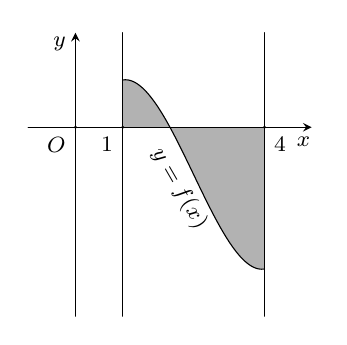
\begin{tikzpicture}[scale=0.6,>=stealth,line join=round,line cap=round,font=\footnotesize]
			\def\xmin{-1} 
			\def\xmax{5}
			\def\ymin{-4} 
			\def\ymax{2} 
			\def\f{1/3*(\x)^3-5/2*(\x)^2+25/6*(\x)-1}
			\fill [gray!60] plot [domain=1:4] (\x, {\f})--(4,0)--(1,0)--cycle;
			\draw [smooth, samples=100] plot [domain=1:4] (\x, {\f});
			\draw (1,\ymin)--(1,\ymax) (4,\ymin)--(4,\ymax);
			\fill (1,0) circle (1pt) node [below left] {$1$} (4,0) circle (1pt) node [below right] {$4$} (2.2,-1.3) node [rotate=-60] {$y=f(x)$};
			\draw [->] (\xmin,0)--(\xmax,0) node [below, xshift=-3pt] {$x$};
			\draw [->] (0,\ymin)--(0,\ymax) node [left, yshift=-4pt] {$y$};
			\fill [black] (0,0) circle (1pt) node [below left] {$O$};
		\end{tikzpicture}
	}
	\loigiai{
		Hình phẳng giới hạn bởi đồ thị hàm số $y=f(x)$, trục hoành và hai đường thẳng $x=1$, $x=4$ nên diện tích được tính theo công thức $S=\displaystyle\int\limits_{1}^{4}{\big|f(x)\big|}\mathrm{\,d}{x}$.
	}
\end{ex}
\begin{ex}%[2D4N3-1]%[Dự án đề cương 3 khối NH24-25-Dot1-Trương Tường]
	\immini{
		Công thức nào sau đây tính diện tích phần hình phẳng được tô đậm ở hình bên?
		\choice[2]
		{$S=\displaystyle\int\limits_{0}^{\tfrac{\pi}{2}}{\big|\sin{x}\big|}\mathrm{\,d}{x}$}
		{$S=\displaystyle\int\limits_{-\tfrac{\pi}{2}}^{0}{\big|\sin{x}\big|}\mathrm{\,d}{x}$}
		{\True $S=\displaystyle\int\limits_{-\tfrac{\pi}{2}}^{\tfrac{\pi}{2}}{\big|\sin{x}\big|}\mathrm{\,d}{x}$}
		{$S=\displaystyle\int\limits_{-\tfrac{\pi}{2}}^{\tfrac{\pi}{2}}{\sin{x}}\mathrm{\,d}{x}$}
	}
	{
		\begin{tikzpicture}[scale=1,>=stealth,line join=round,line cap=round,font=\footnotesize]
			\def\xmin{-3} 
			\def\xmax{3}
			\def\ymin{-2} 
			\def\ymax{2} 
			\def\f{sin(\x r)}
			\fill [gray!60] plot [domain=-pi/2:pi/2] (\x, {\f})--(pi/2,0)--(-pi/2,0)--cycle;
			\draw [smooth, samples=100] plot [domain=-pi/2:pi/2] (\x, {\f});
			\fill (-pi/2,0) circle (1pt) node [below left] {$-\dfrac{\pi}{2}$} (pi/2,0) circle (1pt) node [below right] {$\dfrac{\pi}{2}$} (.7,.8) node [rotate=35] {$y=\sin{x}$};
			\draw (-pi/2,\ymin)--(-pi/2,\ymax) (pi/2,\ymin)--(pi/2,\ymax);
			\draw [->] (\xmin,0)--(\xmax,0) node [below, xshift=-3pt] {$x$};
			\draw [->] (0,\ymin)--(0,\ymax) node [left, yshift=-4pt] {$y$};
			\fill [black] (0,0) circle (1pt) node [above left] {$O$};
		\end{tikzpicture}
	}
	\loigiai{
		Hình phẳng  giới hạn bởi đồ thị hàm số $y=\sin x$, trục hoành và hai đường thẳng $x=-\dfrac{\pi}{2}$, $x=\dfrac{\pi}{2}$ nên diện tích được tính theo công thức $S=\displaystyle\int\limits_{-\tfrac{\pi}{2}}^{\tfrac{\pi}{2}}{\big|\sin{x}\big|}\mathrm{\,d}{x}$.
	}
\end{ex}
\begin{ex}%[2D4N3-1]%[Dự án đề cương 3 khối NH24-25-Dot1-Trương Tường]
	Gọi $(H)$ là hình phẳng giới hạn bởi đồ thị hai hàm số $y=2^{x}$, $y=x-3$, trục tung và đường thẳng $x=2$. Diện tích $S$ của hình phẳng $(H)$ được tính theo công thức nào sau đây? 
	\choice
	{$S=\displaystyle\int\limits_{2}^{0}{\left|2^x-x-3\right|}\mathrm{\,d}{x}$}
	{\True $S=\displaystyle\int\limits_{0}^{2}{\left|2^x-x+3\right|}\mathrm{\,d}{x}$}
	{$S=\displaystyle\int\limits_{0}^{2}{\left|2^x+x-3\right|}\mathrm{\,d}{x}$}
	{$S=\displaystyle\int\limits_{0}^{2}{\left|2^x+x+3\right|}\mathrm{\,d}{x}$}
	\loigiai{
		Hình phẳng $(H)$ giới hạn bởi đồ thị hai hàm số $y=2^{x}$, $y=x-3$, trục tung ($x=0$) và đường thẳng $x=2$ nên diện tích được tính theo công thức $S=\displaystyle\int\limits_{0}^{2}{\left|2^x-(x-3)\right|}\mathrm{\,d}{x}=\displaystyle\int\limits_{0}^{2}{\left|2^x-x+3\right|}\mathrm{\,d}{x}$.
	}
\end{ex}
\begin{ex}%[2D4N3-1]%[Dự án đề cương 3 khối NH24-25-Dot1-Trương Tường]
	\immini{
		Công thức nào sau đây tính diện tích phần hình phẳng được gạch sọc ở hình bên?
		\choice[2]
		{$S=\displaystyle\int\limits_{b}^{a}{\left|f(x)+g(x)\right|}\mathrm{\,d}{x}$}
		{\True $S=\displaystyle\int\limits_{b}^{a}{\left|f(x)-g(x)\right|}\mathrm{\,d}{x}$}
		{$S=\displaystyle\int\limits_{a}^{b}{\left|f(x)+g(x)\right|}\mathrm{\,d}{x}$}
		{$S=\displaystyle\int\limits_{a}^{b}{\left|f(x)-g(x)\right|}\mathrm{\,d}{x}$}
	}
	{
		\begin{tikzpicture}[scale=.6,>=stealth,line join=round,line cap=round,font=\footnotesize]
			\def\xmin{-1} 
			\def\xmax{5}
			\def\ymin{-1} 
			\def\ymax{6}
			\clip (\xmin,\ymin) rectangle (\xmax,\ymax); 
			\def\f{(\x)^2-4*(\x)+5}
			\def\g{\x+1}
			\fill [pattern=north west lines] plot [domain=1:4] (\x, {\f}) -- plot[domain=4:1] (\x, {\g});
			\draw [smooth, samples=100] plot [domain=\xmin:\xmax] (\x, {\f}) plot [domain=\xmin:\xmax] (\x, {\g});
			\fill (1,0) circle (1pt) node [below] {$b$} (4,0) circle (1pt) node [below] {$a$} (2.3,4) node [rotate=45] {$y=f(x)$} (3.3,1.9) node [rotate=65] {$y=g(x)$};
			\draw [->] (\xmin,0)--(\xmax,0) node [below, xshift=-3pt] {$x$};
			\draw [->] (0,\ymin)--(0,\ymax) node [left, yshift=-4pt] {$y$};
			\fill [black] (0,0) circle (1pt) node [below left] {$O$};
			\draw [dashed] (1,0)--(1,2) (4,0)--(4,5);
		\end{tikzpicture}
	}
	\loigiai{
		Hình phẳng giới hạn bởi đồ thị hai hàm số $y=f(x)$, $y=g(x)$ và hai đường thẳng $x=b$, $x=a$ $(b<a)$ nên diện tích được tính theo công thức $S=\displaystyle\int\limits_{b}^{a}{\left|f(x)-g(x)\right|}\mathrm{\,d}{x}$.
	}
\end{ex}
\begin{ex}%[2D4N3-4]%[Dự án đề cương 3 khối NH24-25-Dot1-Trương Tường]
	(\textit{Trích đề thi HKII - Trường THPT Lương Ngọc Quyến – Thái Nguyên - Năm học 2024–2025}) \\
	Cho một vật thể trong không gian $Oxyz$. Gọi $\beta$ là phần vật thể giới hạn bởi hai mặt phẳng vuông góc với trục $Ox$ tại các điểm có hoành độ $x=a$, $x=b$. Một mặt phẳng vuông góc với trục $Ox$ tại điểm có hoành độ là $x$ cắt vật thể theo mặt cắt có diện tích là $S(x)$. Giả sử $S(x)$ là hàm số liên tục trên đoạn $[a;b]$. Khi đó, thể tích $V$ của phần vật thể $\beta$ tính bởi công thức là
	\choice
	{$V=\pi\displaystyle\int\limits_a^b S(x)\mathrm{\,d}{x}$}
	{$V=\pi\displaystyle\int\limits_a^b S^2(x)\mathrm{\,d}{x}$}
	{$V=S'(x)$}
	{\True $V=\displaystyle\int\limits_a^b S(x)\mathrm{\,d}{x}$}
	\loigiai{
		Áp dụng công thức tính thể tích vật thể, ta có $V=\displaystyle\int\limits_a^b S(x) \mathrm{\,d}{x}$.
	}
\end{ex}
\begin{ex}%[2D4N3-4]%[Dự án đề cương 3 khối NH24-25-Dot1-Trương Tường]
	Trong không gian tọa độ $Oxyz$, xét vật thể nằm giữa hai mặt phẳng vuông góc với trục hoành  tại điểm $x=1$ và $x=4$. Khi cắt vật thể bởi mặt phẳng vuông góc với trục hoành tại điểm có hoành độ $x$ $(1 \le x \le 4)$ ta được thiết diện có diện tích $S(x)=4x^3$. Thể tích của vật thể đó bằng 
	\choice
	{$256$}
	{\True $255$}
	{$64$}
	{$63$}
	\loigiai{
		Áp dụng công thức tính thể tích vật thể, ta có
		$$V=\displaystyle\int\limits_{1}^{4}\left(4x^3\right)\mathrm{\,d}{x}
		= x^4\Bigg|_{1}^{4}
		= 4^4 - 1^4 = 255.$$
	}
\end{ex}
\begin{ex}%[2D4N3-3]%[Dự án đề cương 3 khối NH24-25-Dot1-Trương Tường]
	\immini{
		Trong mặt phẳng tọa độ $Oxy$, gọi $(H)$ là phần hình phẳng được tô đậm ở hình bên. Khi quay hình $(H)$ quanh trục hoành ta được khối tròn xoay có thể tích $V$ được tính theo công thức nào sau đây?
		\choice[2]
		{$V=\displaystyle\int\limits_{-1}^{3}{\big[f(x)\big]^2}\mathrm{\,d}{x}$}
		{\True $V=\pi\displaystyle\int\limits_{-1}^{3}{\big[f(x)\big]^2}\mathrm{\,d}{x}$}
		{$V=\pi\displaystyle\int\limits_{-1}^{3}{f(x)}\mathrm{\,d}{x}$}
		{$V=\displaystyle\int\limits_{-1}^{3}{f(x)}\mathrm{\,d}{x}$}
	}
	{
		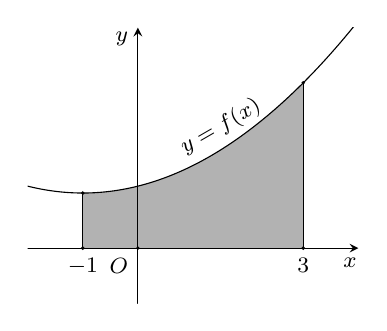
\begin{tikzpicture}[scale=0.7,>=stealth,line join=round,line cap=round,font=\footnotesize]
			\def\xmin{-2} 
			\def\xmax{4}
			\def\ymin{-1} 
			\def\ymax{4} 
			\clip (\xmin,\ymin) rectangle (\xmax,\ymax);
			\def\f{1/8*(\x)^2+1/4*(\x)+9/8}
			\fill [gray!60] plot [domain=-1:3] (\x,{\f})--(3,0)--(-1,0)--cycle;
			\draw [smooth,samples=100] plot [domain=\xmin:\xmax] (\x,{\f});
			\draw [->] (\xmin,0)--(\xmax,0) node [below, xshift=-3pt] {$x$};
			\draw [->] (0,\ymin)--(0,\ymax) node [left, yshift=-4pt] {$y$};
			\fill [black] (0,0) circle (1pt) node [below left] {$O$} (-1,0) circle (1pt) node [below] {$-1$} (3,0) circle (1pt) node [below] {$3$} (-1,1) circle (1pt) (3,3) circle (1pt) (1.5,2.2) node [rotate=30] {$y=f(x)$};
			\draw (-1,0)--(-1,1) (3,0)--(3,3);
		\end{tikzpicture}
	}
	\loigiai{
		Hình phẳng $(H)$ giới hạn bởi đồ thị hàm số $y=f(x)$, trục hoành và hai đường thẳng $x=-1$, $x=3$. \\
		Áp dụng công thức tính thể tích khối tròn xoay, ta có thể tích cần tìm là $V=\pi\displaystyle\int\limits_{-1}^{3}{\big[f(x)\big]^2}\mathrm{\,d}{x}$.
	}
\end{ex}
\begin{ex}%[2D4N3-3]%[Dự án đề cương 3 khối NH24-25-Dot1-Trương Tường]
	Trong mặt phẳng tọa độ $Oxy$, gọi $(D)$ là phần hình phẳng được giới hạn bởi đồ thị hàm số $y=3^x$, trục hoành và hai đường thẳng $x=0$, $x=3$. Khi quay hình $(D)$ quanh trục hoành ta được khối tròn xoay có thể tích $V$ được tính theo công thức nào sau đây?
	\choice
	{$V=\displaystyle\int\limits_{0}^{3}3^x\mathrm{\,d}{x}$}
	{\True $V=\pi\displaystyle\int\limits_{0}^{3}9^x\mathrm{\,d}{x}$}
	{$V=\displaystyle\int\limits_{0}^{3}9^x\mathrm{\,d}{x}$}
	{$V=\pi\displaystyle\int\limits_{0}^{3}3^x\mathrm{\,d}{x}$}
	\loigiai{
		Áp dụng công thức tính thể khối tròn xoay, ta có 
		$$V=\pi\displaystyle\int\limits_{0}^{3}\left(3^x\right)^2\mathrm{\,d}{x}
		=\pi\displaystyle\int\limits_{0}^{3}9^x\mathrm{\,d}{x}.$$
	}
\end{ex}
\begin{ex}%[2D4N3-3]%[Dự án đề cương 3 khối NH24-25-Dot1-Trương Tường]
	Trong không gian $Oxyz$, một khối tròn xoay được tạo thành khi quay quanh trục hoành phần hình phẳng giới hạn bởi đồ thị hàm số $y=\dfrac{1}{x}$, trục hoành và hai đường thẳng $x=1$, $x=4$ như hình bên dưới. \\
	\centerline{
		\begin{tikzpicture}[scale=1.5,>=stealth,line join=round,line cap=round,font=\footnotesize]
			%% Xây dựng hệ tọa độ Oxyz
			\def\g{-1.5}
			\def\r{.996}
			\pgfmathsetmacro\ra{sqrt(1-(\r)^2)}
			\pgfmathsetmacro\a{cos(\g)}
			\pgfmathsetmacro\b{sin(\g)}
			\pgfmathsetmacro\ax{\ra*cos(\g)/sqrt((\ra*\a)^2+(\b)^2)}
			\pgfmathsetmacro\bx{\ra*sin(\g)/sqrt((\ra*\a)^2+(\b)^2)}
			% Định nghĩa giá trị min -max trên trục tọa độ
			\def\xmax{5}
			\def\ymax{2}
			\def\zmax{6}
			% Cận
			\def\m{1}
			\def\n{4}
			% Định nghĩa các hàm số 
			\pgfmathdeclarefunction{h}{1}{%
				\pgfmathparse{1/(#1)} 
			}
			% Định nghĩa vectơ đơn vị và các điểm khác
			\path 
			(0,0) coordinate (O)
			+({\ax},{\bx}) coordinate (i)
			+({\bx/\ra},{-\ax*\ra}) coordinate (k)
			+(0,{\r}) coordinate (j)
			;
			% Vẽ
			\fill [orange!60!black!80, smooth, samples=80,opacity=.5] plot [domain={\m}:{\n}] ({\ax*\x}, {h(\x)*\r+\x*\bx})
			--($\n*(i)$)--($\m*(i)$)--cycle
			;
			\begin{scope}
				\pgfmathsetmacro{\Rn}{h(\n)}
				\pgfmathsetmacro{\Rm}{h(\m)}
				\def\i{sqrt((\Rn)^2-(\x)^2)}
				\def\j{sqrt((\Rm)^2-(\x)^2)}
				\fill [cyan, smooth, samples=80, opacity=.6] plot [domain={0}:{\Rn}] ({\x*\bx/\ra+\n*\ax}, {\n*\bx-\x*\ax*\ra+\i*\r})
				--plot [domain={\Rn}:{0}] ({\x*\bx/\ra+\n*\ax}, {\n*\bx-\x*\ax*\ra-\i*\r})
				--plot [domain={\n}:{\m}] ({\ax*\x}, {-h(\x)*\r+\x*\bx})
				--plot [domain={0}:{\Rm}] ({\x*\bx/\ra+\m*\ax}, {\m*\bx-\x*\ax*\ra-\j*\r})
				--plot [domain={\Rm}:{0}] ({\x*\bx/\ra+\m*\ax}, {\m*\bx-\x*\ax*\ra+\j*\r})
				--plot [domain={\m}:{\n}] ({\ax*\x}, {h(\x)*\r+\x*\bx})--cycle
				;
				\fill [cyan!60, smooth, samples=80, opacity=.5] plot [domain={0}:{-\Rn}] ({\x*\bx/\ra+\n*\ax}, {\n*\bx-\x*\ax*\ra+\i*\r})
				--plot [domain={-\Rn}:{0}] ({\x*\bx/\ra+\n*\ax}, {\n*\bx-\x*\ax*\ra-\i*\r})
				--plot [domain={\n}:{\m}] ({\ax*\x}, {-h(\x)*\r+\x*\bx})
				--plot [domain={0}:{-\Rm}] ({\x*\bx/\ra+\m*\ax}, {\m*\bx-\x*\ax*\ra-\j*\r})
				--plot [domain={-\Rm}:{0}] ({\x*\bx/\ra+\m*\ax}, {\m*\bx-\x*\ax*\ra+\j*\r})
				--plot [domain={\m}:{\n}] ({\ax*\x}, {h(\x)*\r+\x*\bx})--cycle
				;
				\draw [smooth, samples=80, opacity=.5] 
				plot [domain={-\Rn}:{\Rn}] ({\x*\bx/\ra+\n*\ax}, {\n*\bx-\x*\ax*\ra+\i*\r})
				--plot [domain={\Rn}:{-\Rn}] ({\x*\bx/\ra+\n*\ax}, {\n*\bx-\x*\ax*\ra-\i*\r})--cycle
				plot [domain={0}:{\Rm}] ({\x*\bx/\ra+\m*\ax}, {\m*\bx-\x*\ax*\ra-\j*\r}) coordinate (t)
				--plot [domain={\Rm}:{0}] ({\x*\bx/\ra+\m*\ax}, {\m*\bx-\x*\ax*\ra+\j*\r})
				;
				\draw [smooth, samples=80, opacity=.5, dash pattern=on 1pt off 1pt] 
				plot [domain={0}:{-\Rm}] ({\x*\bx/\ra+\m*\ax}, {\m*\bx-\x*\ax*\ra-\j*\r})
				--plot [domain={-\Rm}:{0}] ({\x*\bx/\ra+\m*\ax}, {\m*\bx-\x*\ax*\ra+\j*\r})
				;
			\end{scope}
			\begin{scope}
				\foreach \k in {.5,1,2,4}{
					\pgfmathsetmacro\t{sqrt(1+(\k)^2)}
					\draw [smooth, samples=80, very thin, gray] plot [domain={\m}:{\n}] ({\ax*\x+\k*h(\x)/\t*\bx/\ra}, {h(\x)/\t*\r+\x*\bx-\k*h(\x)/\t*\ax*\ra})
					;
					\draw [smooth, samples=80, very thin, gray] plot [domain={\m}:{\n}] ({\ax*\x+\k*h(\x)/\t*\bx/\ra}, {-h(\x)/\t*\r+\x*\bx-\k*h(\x)/\t*\ax*\ra})
					;
				}
			\end{scope}
			\draw [smooth, samples=80, very thin, gray] plot [domain={\m}:{\n}] ({\ax*\x+h(\x)*\bx/\ra}, {\bx*\x-h(\x)*\ax*\ra})
			;
			%	
			\draw [smooth, samples=80, gray] plot [domain={\n}:{\m}] ({\ax*\x}, {-h(\x)*\r+\x*\bx})
			plot [domain={\n}:{\m}] ({\ax*\x}, {h(\x)*\r+\x*\bx});
			% Vẽ hệ trục
			\draw [gray] ($\n*(i)$)--({\n*\ax},{\n*\bx+h(\n)*\r});
			\draw [dash pattern=on 1pt off 1pt, gray] ($\m*(i)$)--({\m*\ax},{\m*\bx+h(\m)*\r});
			\draw [->] ($\n*(i)$)--($\xmax*(i)$) node [right] {$x$};
			\draw (O)--($\m*(i)$);
			\draw [dash pattern=on 1pt off 1pt, gray] ($\m*(i)$)--($\n*(i)$);
			\draw [->] (O)--($\zmax*(k)$) node [left] {$z$};
			\draw [->] (O)--($\ymax*(j)$) node [left] {$y$};
			\fill (O) circle (1pt) node [above left] {$O$}
			(i) circle (1pt) node [below] {$1$}
			($\n*(i)$) node [below right] {$4$};
		\end{tikzpicture}
	}
	Thể tích của khối tròn xoay đó bằng
	\choice 
	{$\dfrac{3}{4}$}
	{\True $\dfrac{3\pi}{4}$}
	{$\dfrac{5\pi}{4}$}
	{$\dfrac{5}{4}$}
	\loigiai{
		Áp dụng công thức tính thể tích khối tròn xoay ta có 
		$$V=\pi\displaystyle\int\limits_{1}^{4}\dfrac{1}{x^2}\mathrm{\,d}{x}=\dfrac{3\pi}{4}.$$
	}
\end{ex}
%----Mức độ Thông hiểu-----%
\begin{ex}%[2D4H3-1]%[Dự án đề cương 3 khối NH24-25-Dot1-Trương Tường]
	(\textit{Trích đề thi HKII - Trường THPT Hùng Thắng – Hải Phòng - Năm học 2024-2025})
	\immini{
		Cho hàm số $f(x)$ liên tục trên $\mathbb{R}$. Gọi $S$ là diện tích hình phẳng giới hạn bởi các đường $y=f(x)$, trục hoành và hai đường thẳng $x=-2$, $x=3$ (như hình vẽ). Mệnh đề nào dưới đây đúng?
		\choice[2]
		{$S=\displaystyle\int\limits_{-2}^{-1} f(x)\mathrm{\,d}{x}+\int\limits_{1}^{3} f(x)\mathrm{\,d}{x}$}
		{\True $S=\displaystyle\int\limits_{-2}^{1} f(x)\mathrm{\,d}{x}-\int\limits_{1}^{3} f(x)\mathrm{\,d}{x}$}
		{$S=-\displaystyle\int\limits_{-2}^{-1} f(x)\mathrm{\,d}{x}-\int\limits_{1}^{3} f(x)\mathrm{\,d}{x}$}
		{$S=-\displaystyle\int\limits_{-2}^{1} f(x)\mathrm{\,d}{x}+\int\limits_{1}^{3} f(x)\mathrm{\,d}{x}$}
	}
	{
		\begin{tikzpicture}[scale=0.4,>=stealth,line join=round,line cap=round,font=\footnotesize]
			\def\xmin{-4} 
			\def\xmax{5}
			\def\ymin{-3} 
			\def\ymax{6} 
			\clip (\xmin,\ymin) rectangle (\xmax,\ymax);
			\def\f{(\x+2)*(\x-1)*(\x-3)/2}
			\fill [smooth, samples=100, pattern=north west lines] plot [domain=-2:3] (\x, {\f})--cycle;
			\draw [smooth, samples=100] plot [domain=\xmin:\xmax] (\x, {\f});
			\draw [->] (\xmin,0)--(\xmax,0) node [below, xshift=-3pt] {$x$};
			\draw [->] (0,\ymin)--(0,\ymax) node [left, yshift=-4pt] {$y$};
			\fill [black] (0,0) circle (1pt) node [below left] {$O$}
			(-2,0) circle (1pt) node [below left] {$-2$}
			(1,0) circle (1pt) node  [below left] {$1$}
			(3,0) circle (1pt) node [below right] {$3$};
		\end{tikzpicture}
	}
	\loigiai{
		Diện tích hình phẳng cần tìm là 
		\begin{eqnarray*}
			&S&=\displaystyle\int\limits_{-2}^{3}|f(x)|\mathrm{\,d}{x} \\
			&&=\displaystyle\int\limits_{-2}^{1}|f(x)|\mathrm{\,d}{x}+\displaystyle\int\limits_{1}^{3}|f(x)|\mathrm{\,d}{x}.  
		\end{eqnarray*}
		Từ đồ thị hàm số $f(x)$ ta có: $f(x) \ge 0, \; \forall x \in  [-2;1]$ và  $f(x) \le 0, \; \forall x \in [1;3]$ nên 
		$$S=\displaystyle\int\limits_{-2}^{1}f(x)\mathrm{\,d}{x}-\displaystyle\int\limits_{1}^{3}f(x)\mathrm{\,d}{x}.$$
	}
\end{ex}
\begin{ex}%[2D4H3-1]%[Dự án đề cương 3 khối NH24-25-Dot1-Trương Tường]
	\immini{
		Công thức nào sau đây tính diện tích phần hình phẳng được gạch sọc ở hình bên?
		\choice[2]
		{$S=\displaystyle\int\limits_{-1}^{2}{\Bigg|2^{x}-\dfrac{7}{6}x+\dfrac{5}{3}\Bigg|}\mathrm{\,d}{x}$}
		{$S=\displaystyle\int\limits_{-1}^{2}{\left(2^{x}-\dfrac{7}{6}x-\dfrac{5}{3}\right)}\mathrm{\,d}{x}$}
		{$S=\displaystyle\int\limits_{-1}^{2}{\Bigg|\dfrac{7}{6}x+\dfrac{5}{3}+2^{x}\Bigg|}\mathrm{\,d}{x}$}
		{\True $S=\displaystyle\int\limits_{-1}^{2}{\left(\dfrac{7}{6}x+\dfrac{5}{3}-2^{x}\right)}\mathrm{\,d}{x}$}
	}
	{
		\begin{tikzpicture}[scale=.7,>=stealth,line join=round,line cap=round,font=\footnotesize]
			\def\xmin{-3} 
			\def\xmax{3}
			\def\ymin{-1} 
			\def\ymax{5}
			\clip (\xmin,\ymin) rectangle (\xmax,\ymax); 
			\def\f{2^(\x)}
			\def\g{7/6*(\x)+5/3}
			\fill [pattern=north west lines] plot [domain=-1:2] (\x, {\f}) -- plot[domain=2:-1] (\x, {\g});
			\draw [smooth, samples=100] plot [domain=\xmin:\xmax] (\x, {\f}) plot [domain=\xmin:\xmax] (\x, {\g}) node [above left,yshift=-1pt] {$y=1$};
			\draw [->] (\xmin,0)--(\xmax,0) node [below, xshift=-3pt] {$x$};
			\draw [->] (0,\ymin)--(0,\ymax) node [left, yshift=-4pt] {$y$};
			\fill [black] (0,0) circle (1pt) node [below left] {$O$};
			\draw [dashed] (-1,0)--(-1,.5) (2,0)--(2,4);
			\fill (-1,0) circle (1pt) node [below] {$-1$} (2,0) circle (1pt) node [below] {$2$} (-1,.5) circle (1pt) (2,4) circle (1pt) (1,1.5) node [rotate=50] {$y=2^{x}$} (-.5,2.5) node [fill=white,inner sep=0pt,rotate=atan(7/6)] {$y=\dfrac{7}{6}x+\dfrac{5}{3}$};
		\end{tikzpicture}
	}
	\loigiai{
		Phần hình phẳng được giới hạn bởi đồ thị hai hàm số $y=\dfrac{7}{6}x+\dfrac{5}{3}$, $y=2^x$ và hai đường thẳng $x=-1$, $x=2$ nên diện tích được tính theo công thức 
		$$S=\displaystyle\int\limits_{-1}^{2}\left|\dfrac{7}{6}x+\dfrac{5}{3}-2^x\right|\mathrm{\,d}{x}.$$
		Từ đồ thị ta có $\dfrac{7}{6}x+\dfrac{5}{3} \ge 2^x, \; \forall x \in [-1;2]$ nên 
		$$S=\displaystyle\int\limits_{-1}^{2}\left(\dfrac{7}{6}x+\dfrac{5}{3}-2^x\right)\mathrm{\,d}{x}.$$
	}
\end{ex}
\begin{ex}%[2D4H3-3]%[Dự án đề cương 3 khối NH24-25-Dot1-Trương Tường]
	Gọi $(H)$ là hình phẳng giới hạn bởi đồ thị hàm số $y=x^2-2x$ và trục hoành. Khi quay hình $(H)$ quanh trục hoành ta được một vật thể tròn xoay có thể tích $V$ bằng bao nhiêu?
	\choice
	{\True $V=\dfrac{16\pi}{15}$}
	{$V=\dfrac{8\pi}{15}$}
	{$V=\dfrac{4\pi}{15}$}
	{$V=\dfrac{7\pi}{15}$}
	\loigiai{
		Xét phương trình $x^2-2x=0 \Leftrightarrow x=0, \; x=2$. \\
		Hình phẳng $(H)$ được giới hạn bởi đồ thị hàm số $y=x^2-2x$, trục hoành và hai đường thẳng $x=0$, $x=2$. \\
		Thể tích khối tròn xoay cần tìm là 
		$$V=\pi\displaystyle\int\limits_{0}^{2}\left(x^2-2x\right)^2\mathrm{\,d}{x}=\dfrac{16\pi}{15}.$$ 
	}
\end{ex}
\begin{ex}%[2D4H3-4]%[Dự án đề cương 3 khối NH24-25-Dot1-Trương Tường]
	Khi cắt một vật thể bởi mặt phẳng vuông góc với trục $Ox$ tại điểm có hoành độ $x$, với $-\sqrt{3} \le x \le \sqrt{3}$ ta được thiết diện là hình vuông có độ dài cạnh là $\sqrt{3-x^{2}}$. Thể tích của vật thể đã cho bằng
	\choice
	{$\pi\sqrt{3}$}
	{$\sqrt{3}$}
	{$\dfrac{4\pi}{3}$}
	{\True $4\sqrt{3}$}
	\loigiai{
		Diện tích thiết diện là $S(x)=\left(\sqrt{3-x^2}\right)^2=3-x^2$. \\
		Thể tích vật thể đã cho là  
		$$V=\displaystyle\int\limits_{-\sqrt{3}}^{\sqrt{3}}\left(3-x^2\right)\mathrm{\,d}{x}=4\sqrt{3}.$$
	}
\end{ex}
\begin{ex}%[2D4H3-3]%[Dự án đề cương 3 khối NH24-25-Dot1-Trương Tường]
	\immini{
		Gọi $(H)$ là phần hình phẳng gạch sọc như hình vẽ bên. Khi quay hình $(H)$ quanh trục hoành ta được một vật thể tròn xoay có thể tích $V$ bằng bao nhiêu?
		\choice[2]
		{$V=\dfrac{16}{3}$}
		{$V=\dfrac{16\pi}{3}$}
		{\True $V=8\pi $}
		{$V=8$}
	}
	{
		\begin{tikzpicture}[scale=0.7,line join=round,line cap=round,>=stealth,font=\footnotesize]
			\def\xmin{-1}
			\def\xmax{6}
			\def\ymin{-1}
			\def\ymax{3}
			\def\f{sqrt(\x)}
			\fill[pattern=north west lines] plot [domain=0:4] (\x,{\f})--plot [domain=4:0] (\x,0)--cycle;
			\draw[smooth, samples=100] plot [domain=0:\xmax] (\x,{\f}) node [below left,rotate=10] {$y=\sqrt{x}$};
			\draw [->] (\xmin,0)--(\xmax,0) node [below, xshift=-3pt] {$x$};
			\draw [->] (0,\ymin)--(0,\ymax) node [left, yshift=-4pt] {$y$};
			\draw (4,\ymin)--(4,\ymax) node [right] {$x=4$};
			\fill (0,0) circle (1pt) node [below left] {$O$}
			(4,0) circle (1pt) node [below right] {$4$};
		\end{tikzpicture}
	}
	\loigiai{
		Hình phẳng $(H)$ giới hạn bởi đồ thị hàm số $y=\sqrt{x}$, trục hoành và hai đường thẳng $x=0$, $x=4$. \\
		Thể tích vật thể tròn xoay cần tìm là 
		$$V=\pi\displaystyle\int\limits_{0}^{4}\left(\sqrt{x}\right)^2\mathrm{\,d}{x}=8\pi.$$
	}
\end{ex}
\begin{ex}%[2D4H3-1]%[Dự án đề cương 3 khối NH24-25-Dot1-Trương Tường]
	Cho tích phân $S=\displaystyle\int\limits_{-3}^{3}{\sqrt{9-x^{2}}}\mathrm{\,d}{x}$ (đơn vị diện tích). Khẳng định nào sau đây là đúng?
	\choice
	{\True $S$ là diện tích nửa hình tròn tâm $O(0;0)$, bán kính $R=3$}
	{$S$ là diện tích nửa hình tròn tâm $O(0;0)$, bán kính $R=6$}
	{$S$ là diện tích hình tròn tâm $O(0;0)$, bán kính $R=3$}
	{$S$ là diện tích hình tròn tâm $O(0;0)$, bán kính $R=6$}
	\loigiai{
		$S=\displaystyle\int\limits_{-3}^{3}{\sqrt{9-x^{2}}}\mathrm{\,d}{x}$ là công thức tính diện tích hình phẳng giới hạn bởi đồ thị hàm số $y=\sqrt{9-x^2}$, trục hoành và hai đường thẳng $x=\pm 3$. \\
		Mà $y=\sqrt{9-x^2}$ là phương trình nửa đường tròn tâm $O$ bán kính $R=3$ (nằm phía trên trục hoành) nên $S$ là diện tích nửa hình tròn tâm $O(0;0)$, bán kính $R=3$. 
	}
\end{ex}
\begin{ex}%[2D4H3-3]%[Dự án đề cương 3 khối NH24-25-Dot1-Trương Tường]
	\immini{
		Trong mặt phẳng tọa độ $Oxy$, gọi $(H)$ là hình chữ nhật được tô đậm ở hình bên. Khi quay hình $(H)$ quanh trục hoành ta được khối tròn xoay có thể tích $V$ được tính theo công thức nào sau đây?
		\choice[2]
		{$V=\pi\displaystyle\int\limits_{-2}^{2}\mathrm{\,d}{x}$}
		{\True $V=\pi\displaystyle\int\limits_{-2}^{2}{4}\mathrm{\,d}{x}$}
		{$V=\pi\displaystyle\int\limits_{-2}^{2}{2}\mathrm{\,d}{x}$}
		{$V=\displaystyle\int\limits_{-2}^{2}{2}\mathrm{\,d}{x}$}
	}
	{
		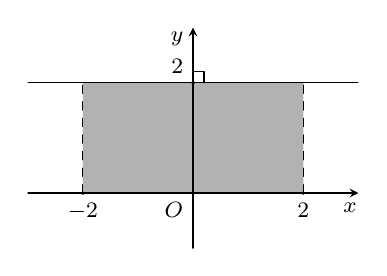
\begin{tikzpicture}[scale=0.7,>=stealth,line join=round,line cap=round,font=\footnotesize]
			\def\xmin{-3} 
			\def\xmax{3}
			\def\ymin{-1} 
			\def\ymax{3} 
			\clip (\xmin,\ymin) rectangle (\xmax,\ymax);
			\def\f{2}
			\fill [gray!60] plot [domain=-2:2] (\x,{\f})--(2,0)--(-2,0)--cycle;
			\draw [smooth,samples=200] plot [domain=\xmin:\xmax] (\x,{\f});
			\draw [->] (\xmin,0)--(\xmax,0) node [below, xshift=-3pt] {$x$};
			\draw [->] (0,\ymin)--(0,\ymax) node [left, yshift=-4pt] {$y$};
			\fill [black] (0,0) circle (1pt) node [below left] {$O$} (-2,0) circle (1pt) node [below] {$-2$} (2,0) circle (1pt) node [below] {$2$} (0,2) circle (1pt) node [above left] {$2$};
			\draw [dashed] (-2,0)--(-2,2) (2,0)--(2,2);
			\draw (.2,2)--++(90:.2)--++(180:.2);
		\end{tikzpicture}
	}
	\loigiai{
		Hình chữ nhật là hình phẳng giới hạn bởi đồ thị hàm số $y=2$, trục hoành và hai đường thẳng $x=\pm 2$. \\
		Thể tích cần tìm được tính theo công thức 
		$$V
		=\pi\displaystyle\int\limits_{-2}^{2}{2^2}\mathrm{\,d}{x}
		=\pi\displaystyle\int\limits_{-2}^{2}{4}\mathrm{\,d}{x}.$$
	}
\end{ex}
\begin{ex}%[2D4H3-3]%[Dự án đề cương 3 khối NH24-25-Dot1-Trương Tường]
	(\textit{Trích đề thi HKII - Trường THPT Thị xã Quảng Trị - Năm học 2024-2025}) \\
	Cho hình phẳng $(H)$ giới hạn bởi đồ thị $y=2x-x^2$, trục hoành và hai đường thẳng $x=0$, $x=2$. Tính thể tích $V$ của khối tròn xoay sinh ra khi cho $(H)$ quay quanh trục $Ox$.
	\choice
	{$V=\pi\displaystyle\int\limits_0^2\left(2x-x^2\right)\mathrm{\,d}{x}$}
	{$V=\pi\displaystyle\int\limits_0^2\left(2x-x^2\right)\mathrm{\,d}{x}$}
	{\True $V=\pi\displaystyle\int\limits_0^2\left(2x-x^2\right)^2\mathrm{\,d}{x}$}
	{$V=\displaystyle\int\limits_0^2\left(2x-x^2\right)^2\mathrm{\,d}{x}$}
	\loigiai{
		Áp dụng công thức tính thể tích khối tròn xoay, ta có $V=\pi\displaystyle\int\limits_0^2\left(2x-x^2\right)^2\mathrm{\,d}{x}$.
	}
\end{ex}
\begin{ex}%[2D4H3-1]%[Dự án đề cương 3 khối NH24-25-Dot1-Trương Tường]
	(\textit{Trích đề thi HKII - Sở GD\&ĐT Bắc Ninh - Năm học 2024-2025}) \\
	Tính diện tích hình phẳng giới hạn bởi hai đồ thị hàm số $y=4x-x^2$ và $y=2x$.
	\choice
	{\True $\dfrac{4}{3}$}
	{$4$}
	{$\dfrac{2}{3}$}
	{$\dfrac{16}{3}$}
	\loigiai{
		Xét phương trình $4x-x^2=2x \Leftrightarrow -x^2+2x=0 \Leftrightarrow x=0, \; x=2$. \\
		Hơn nữa, ta có $-x^2+2x \geq 0$, $\forall x \in [0;2]$.\\
		Do đó, diện tích hình phẳng cần tìm là  
		$$S=\displaystyle\int\limits_{0}^{2}\left|\left(4x-x^2\right)-2x\right|\mathrm{\,d}{x}
		=\displaystyle\int\limits_{0}^{2}\left|-x^2+2x\right|\mathrm{\,d}{x} = \displaystyle\int\limits_{0}^{2}\left(-x^2+2x\right)\mathrm{\,d}{x}
		=\dfrac{4}{3}.$$
	}
\end{ex}

\Closesolutionfile{ans}
\indapan{10}{ans/2D4-Bai3-TN}

%%%%%%
\ind{PHẦN II.} \inden{Câu trắc nghiệm đúng sai. Trong mỗi ý a), b), c), d) ở mỗi câu, học sinh chọn đúng hoặc sai.}\\
\setcounter{ex}{0}
\Opensolutionfile{ans}[ans/2D4-Bai3-DS]%
\begin{ex}%[2D4H3-1]%[Dự án đề cương 3 khối NH24-25-Dot1-Trương Tường]
	(\textit{Trích đề ôn tập CK2 - Trường chuyên Lương Văn Chánh – Phú Yên - Năm học 2024-2025})
	\immini{
		Đặt $S$ là diện tích hình phẳng giới hạn bởi đồ thị hàm số $y=f(x)$ và trục hoành (tham khảo hình bên).
		\choiceTF
		{$\displaystyle\int\limits_{-2}^{0}f(x)\mathrm{\,d}{x}>0$}
		{\True $\displaystyle\int\limits_{0}^{3}f(x)\mathrm{\,d}{x}>0$}
		{\True $S=\displaystyle\int\limits_{0}^{-2}f(x)\mathrm{\,d}{x} +\int\limits_{0}^{3}f(x)\mathrm{\,d}{x}$}
		{Nếu $\displaystyle\int\limits_{-2}^{0}f(x)\mathrm{\,d}{x}=-3$, $\displaystyle\int\limits_{0}^{3}f(x)\mathrm{\,d}{x}=6$ thì $S=3$}
	}
	{
		\begin{tikzpicture}[scale=0.7,>=stealth,line join=round,line cap=round,font=\footnotesize]
			\def\xmin{-3} 
			\def\xmax{4}
			\def\ymin{-2} 
			\def\ymax{3} 
			\def\f{-1/4*(\x+2)*(\x)*(\x-3)}
			\clip (\xmin,\ymin) rectangle (\xmax,\ymax);
			\fill [smooth, samples=100, pattern=north west lines] plot [domain=-2:3] (\x, {\f})--cycle;
			\draw [smooth, samples=100] plot [domain=\xmin:\xmax] (\x, {\f})
			plot [samples at={2}] (\x, {\f}) node [above] {$y=f(x)$};
			\draw [->] (\xmin,0)--(\xmax,0) node [below, xshift=-3pt] {$x$};
			\draw [->] (0,\ymin)--(0,\ymax) node [left, yshift=-4pt] {$y$};
			\fill [black] (0,0) circle (1pt) node [above left] {$O$}
			(-2,0) circle (1pt) node [below left] {$-2$}
			(3,0) circle (1pt) node [below left] {$3$};
		\end{tikzpicture}
	}
	\loigiai{
		\begin{itemchoice}
			\itemch \textbf{Sai}. Vì $f(x) < 0, \; \forall x \in (-2;0)$ nên $\displaystyle\int\limits_{-2}^{0}f(x)\mathrm{\,d}{x}<0$. 
			\itemch \textbf{Đúng}. Vì $f(x) > 0, \; \forall x \in (0;3)$ nên $\displaystyle\int\limits_{0}^{3}f(x)\mathrm{\,d}{x}>0$.
			\itemch \textbf{Đúng}. $S=-\displaystyle\int\limits_{-2}^{0}f(x)\mathrm{\,d}{x} +\int\limits_{0}^{3}f(x)\mathrm{\,d}{x}
			=\displaystyle\int\limits_{0}^{-2}f(x)\mathrm{\,d}{x} +\int\limits_{0}^{3}f(x)\mathrm{\,d}{x}$.
			\itemch \textbf{Sai}. $S=-\displaystyle\int\limits_{-2}^{0}f(x)\mathrm{\,d}{x} +\int\limits_{0}^{3}f(x)\mathrm{\,d}{x}
			=-(-3)+6=9$.
		\end{itemchoice}
	}
\end{ex}
\begin{ex}%[2D4V3-3]%[Dự án đề cương 3 khối NH24-25-Dot1-Trương Tường]
	(\textit{Trích đề thi HKII - Sở GD\&ĐT Bình Dương - Năm học 2024-2025}) \\
	Gọi $D$ là hình phẳng giới hạn bởi các đồ thị hàm số $y=\sqrt{x}$, $y=\dfrac{1}{2}\sqrt{x}$ và hai đường thẳng $x=0$, $x=4$.
	\choiceTF
	{\True Gọi $V_1$ là thể tích khối tròn xoay được tạo ra khi quay hình phẳng giới hạn bởi các đường $y=0$, $y=\sqrt{x}$, $x=0$, $x=4$ quanh trục $Ox$. Khi đó $V_1=\pi\displaystyle\int\limits_{0}^{4} x\mathrm{\,d}{x}$}
	{Gọi $V_2$ là thể tích khối tròn xoay được tạo ra khi quay hình phẳng giới hạn bởi các đường $y=0$, $y=\dfrac{1}{2}\sqrt{x}$, $x=0$, $x=4$ quanh trục $Ox$. Khi đó $V_2=\pi\displaystyle\int\limits_{0}^{4} \dfrac{1}{2}x\mathrm{\,d}{x}$}
	{$\dfrac{V_2}{V_1}=\dfrac{1}{2}$}
	{\True Một vật thể được tạo thành khi quay hình phẳng $D$ quanh trục $Ox$. Thể tích của vật thể đó là $18{,}8$ \textit{(kết quả làm tròn đến hàng phần chục)}}
	\loigiai{
		\begin{itemchoice}
			\itemch \textbf{Đúng}. Áp dụng công thức tính thể tích khối tròn xoay, ta có 
			$$V_1=\pi\displaystyle\int\limits_{0}^{4}\left(\sqrt{x}\right)^2\mathrm{\,d}{x}
			=\pi\displaystyle\int\limits_{0}^{4} x\mathrm{\,d}{x}.$$
			\itemch \textbf{Sai}. Áp dụng công thức tính thể tích khối tròn xoay, ta có 
			$$V_2=\pi\displaystyle\int\limits_{0}^{4}\left(\dfrac{1}{2}\sqrt{x}\right)^2\mathrm{\,d}{x}
			=\pi\displaystyle\int\limits_{0}^{4}\dfrac{1}{4}x\mathrm{\,d}{x}.$$
			\itemch \textbf{Sai}. Ta có $V_2=\pi\displaystyle\int\limits_{0}^{4}\dfrac{1}{4}x\mathrm{\,d}{x}
			=\dfrac{1}{4}\pi\displaystyle\int\limits_{0}^{4}x\mathrm{\,d}{x}
			=\dfrac{1}{4}V_1$. \\
			Do đó $\dfrac{V_2}{V_1}=\dfrac{1}{4}$.
			\itemch \textbf{Đúng}. Thể tích vật thể cần tìm là 
			$$V=V_1-V_2=\dfrac{3\pi}{4}\displaystyle\int\limits_{0}^{4}x\mathrm{\,d}{x}=6\pi \approx 18{,}8.$$
		\end{itemchoice}
	}
\end{ex}
\begin{ex}%[2D4V3-3]%[Dự án đề cương 3 khối NH24-25-Dot1-Trương Tường]
	(\textit{Trích đề thi HKII - Sở GD\&ĐT Cần Thơ - Năm học 2024-2025}) \\
	Cho hàm số $y=-x^3+x^2+2x$ có đồ thị $(C)$. Hình phẳng $(H_1)$ được giới hạn bởi $(C)$, trục hoành, hai đường thẳng $x=-1$, $x=0$ và hình phẳng $(H_2)$ được giới hạn bởi $(C)$, trục hoành, hai đường thẳng $x=0$, $x=2$ (như hình vẽ). \\
	\centerline{
		\begin{tikzpicture}[scale=1,>=stealth,line join=round,line cap=round,font=\footnotesize]
			\def\xmin{-2} 
			\def\xmax{3}
			\def\ymin{-1} 
			\def\ymax{2.5}
			\def\f{-(\x+1)*(\x)*(\x-2)}
			\clip (\xmin,\ymin) rectangle (\xmax,\ymax);
			\fill [smooth, samples=100, pattern=north west lines] plot [domain=-1:0] (\x, {\f})--cycle;
			\fill [smooth, samples=100, pattern=north east lines] plot [domain=0:2] (\x, {\f})--cycle;
			\draw [smooth, samples=100] plot [domain=\xmin:\xmax] (\x, {\f});
			\draw [->] (\xmin,0)--(\xmax,0) node [below, xshift=-3pt] {$x$};
			\draw [->] (0,\ymin)--(0,\ymax) node [left, yshift=-4pt] {$y$};
			\fill [black] (0,0) circle (1pt) node [above left] {$O$}
			(-1,0) circle (1pt) node [below left] {$-1$}
			(2,0) circle (1pt) node [below left] {$2$}
			(-.5,-.3) node [fill=white, inner sep=0pt] {$(H_1)$}
			(1,.75) node [fill=white, inner sep=0pt] {$(H_2)$};
			\fill (-1.4,1.8) node[left]{$(C)$};
		\end{tikzpicture}
	}
	\choiceTF
	{Diện tích của hình $(H_1)$ được tính bởi $\displaystyle\int\limits_{-1}^0 \left(-x^3+x^2+2x\right)\mathrm{\,d}{x}$}
	{\True Thể tích của khối tròn xoay được tạo thành khi quay hình $(H_2)$ quanh trục $Ox$ bằng $\dfrac{464}{105}\pi$}
	{Tổng diện tích của hình $(H_1)$ và $(H_2)$ bằng $\dfrac{9}{4}$}
	{\True Gọi $S_1$, $S_2$ lần lượt là diện tích của hình $(H_1)$ và $(H_2)$. Khi đó $S_2>6S_1$}
	\loigiai{
		\begin{itemchoice}
			\itemch \textbf{Sai}. Diện tích của hình $(H_1)$ được tính bởi $\displaystyle\int\limits_{-1}^0 \left|-x^3+x^2+2x\right|\mathrm{\,d}{x}$. \\
			Mà $-x^3+x^2+2x \le 0, \; \forall x \in [-1;0]$ nên
			$$\displaystyle\int\limits_{-1}^0 \left|-x^3+x^2+2x\right|\mathrm{\,d}{x}
			=-\displaystyle\int\limits_{-1}^0 \left(-x^3+x^2+2x\right)\mathrm{\,d}{x}.$$ 
			\itemch \textbf{Đúng}. Thể tích cần tìm là  
			$$V=\pi\displaystyle\int\limits_{0}^{2} \left(-x^3+x^2+2x\right)^2\mathrm{\,d}{x}=\dfrac{464\pi}{105}.$$
			\itemch \textbf{Sai}. Diện tích hình $(H_1)$ là $\displaystyle\int\limits_{-1}^0 \left|-x^3+x^2+2x\right|\mathrm{\,d}{x}=\dfrac{5}{12}.$ \\
			Diện tích hình $(H_2)$ là $\displaystyle\int\limits_{0}^{2} \left|-x^3+x^2+2x\right|\mathrm{\,d}{x}=\dfrac{8}{3}.$ \\
			Tổng diện tích của  $(H_1)$ và $(H_2)$ là $\dfrac{5}{12}+\dfrac{8}{3}=\dfrac{37}{12}.$
			\itemch \textbf{Đúng}. Ta có $S_1=\dfrac{5}{12}$ và $S_2=\dfrac{8}{3}$ suy ra $\dfrac{S_2}{S_1} = \dfrac{\dfrac{8}{3}}{\dfrac{5}{12}} = \dfrac{32}{5} = 6{,}4 > 6 \Rightarrow S_2 > 6S_1$.
		\end{itemchoice}
	}
\end{ex}
\begin{ex}%[2D4V3-3]%[Dự án đề cương 3 khối NH24-25-Dot1-Trương Tường]
	(\textit{Trích đề thi HKII - Sở GD\&ĐT Bắc Ninh - Năm học 2024-2025}) \\
	Cho hình phẳng $(H)$ giới hạn bởi $\dfrac{1}{4}$ đường tròn có bán kính $R=2$, đường cong $y=\sqrt{4-x}$ và trục hoành. Hình phẳng $(H)$ được chia thành hai miền có diện tích là $S_1$ và $S_2$ như hình vẽ. \\
	\centerline{
		\begin{tikzpicture}[scale=0.7,>=stealth,line join=round,line cap=round,font=\footnotesize]
			\def\xmin{-3} 
			\def\xmax{5}
			\def\ymin{-1} 
			\def\ymax{3} 
			\def\f{sqrt(4-\x)}
			\clip (\xmin,\ymin) rectangle (\xmax,\ymax);
			\fill [smooth, samples=100, pattern=north east lines] plot [domain=0:4] (\x, {\f})--(0,0)--cycle;
			\fill [gray!80] (-2,0) arc (-180:-270:{2})--(0,0)--cycle;
			\draw [smooth, samples=100] plot [domain=-1:4] (\x, {\f})
			(-2,0) arc (-180:-270:{2});
			\draw [->] (\xmin,0)--(\xmax,0) node [below, xshift=-3pt] {$x$};
			\draw [->] (0,\ymin)--(0,\ymax) node [left, yshift=-4pt] {$y$};
			\fill [black] (0,0) circle (1pt) node [below left] {$O$}
			(-2,0) circle (1pt) node [below] {$-2$}
			(4,0) circle (1pt) node [below]  {$4$}
			(0,2) circle (1pt) node [above left] {$2$};
			\draw (-1,.7) node [fill=white, inner sep=1pt] {$S_1$}
			(2,.7) node [fill=white, inner sep=1pt] {$S_2$}
			(2,{sqrt(2)}) node [above, rotate=-20] {$y=\sqrt{4-x}$};
		\end{tikzpicture}
	}
	\choiceTF
	{\True Thể tích của khối tròn xoay sinh ra khi quay miền có diện tích $S_2$ quanh trục hoành là $8\pi$}
	{\True Diện tích $S_2=\dfrac{16}{3}$}
	{Thể tích của khối tròn xoay sinh ra khi cho hình $(H)$ quay quanh trục hoành là $\dfrac{28\pi}{3}$}
	{Diện tích $S_1=2\pi$}
	\loigiai{
		\begin{itemchoice}
			\itemch \textbf{Đúng}. Thể tích của khối tròn xoay sinh ra khi quay miền có diện tích $S_2$ quanh trục hoành là
			$$V_2=\pi\displaystyle\int\limits_{0}^{4}\left(\sqrt{4-x}\right)^2\mathrm{\,d}{x}
			=8\pi.$$
			\itemch \textbf{Đúng}. Diện tích $S_2$ là diện tích của hình phẳng được giới hạn bởi đường cong $y=\sqrt{4-x}$, trục hoành và hai đường thẳng $x = 0$, $x = 4$, do đó $$S_2=\displaystyle\int\limits_{0}^{4}\sqrt{4-x}\mathrm{\,d}{x}
			=\dfrac{16}{3}.$$
			\itemch \textbf{Sai}. Phương trình $\dfrac{1}{4}$ đường tròn là $y=\sqrt{4-x^2}$ với $-2 \le x \le 0$. \\
			Thể tích khối tròn xoay sinh ra khi quay miền có diện tích $S_1$ quanh trục hoành là 
			$$V_1=\pi\displaystyle\int\limits_{-2}^{0}\left(\sqrt{4-x^2}\right)^2\mathrm{\,d}{x}=\dfrac{16\pi}{3}.$$
			Thể tích cần tìm là $V=V_1+V_2=\dfrac{40\pi}{3}$.
			\itemch \textbf{Sai}. Phương trình $\dfrac{1}{4}$ đường tròn là $y=\sqrt{4-x^2}$ với $-2 \le x \le 0$.\\
			Diện tích $S_1$ là diện tích của hình phẳng được giới hạn bởi $\dfrac{1}{4}$ đường tròn là $y=\sqrt{4-x^2}$, trục hoành và hai đường thẳng $x = -2$, $x = 0$, do đó $$S_1=\displaystyle\int\limits_{-2}^{0}\sqrt{4-x^2}\mathrm{\,d}{x}=\pi.$$
		\end{itemchoice}
	}
\end{ex}
\begin{ex}%[2D4V3-5]%[Dự án đề cương 3 khối NH24-25-Dot1-Trương Tường]
	\immini{
		Người ta thiết kế một đường hầm sâu $5$ m (khoảng cách giữa lối vào và lối ra là $5$ m) có hình dạng sao cho vào càng sâu thì hầm càng cao. Khi cắt mặt hầm bởi mặt phẳng vuông góc với mặt đất tại điểm cách mặt phẳng chứa lối vào một khoảng $l$ (m) ta được thiết diện là đường parabol có chiều cao $h=1+\dfrac{2l}{5}$ (m) và chiều cao này bằng một nửa độ rộng đáy của parabol. Với mỗi parabol này, chọn hệ tọa độ $Oxy$ sao cho trục $Ox$ chứa giao tuyến của mặt cắt và mặt đất, trục $Oy$ là trục đối xứng của parabol với chiều dương hướng lên từ mặt đất. 
	}
	{
		\begin{tikzpicture}[scale=.6,>=stealth,line join=round,line cap=round,font=\footnotesize]
			\def\xmax{3}
			\def\ymax{3}
			\tikzset{declare function={
					theta=-140;
					r=.95;
					ra=sqrt(1-r^2);
					a=cos(theta);
					b=sin(theta);
					c=sqrt(ra^2*a^2+b^2);
					ax=ra*a/c;
					bx=ra*b/c;
					f=1-(\x)^2;
					g=3-1/3*(\x)^2;
					h=2.2-1/2.2*(\x)^2;
				}
			}
			\path 
			(0,0) coordinate (O)
			+({ax},{bx}) coordinate (i)
			+({bx/ra},{-ax*ra}) coordinate (k)
			+(0,{r}) coordinate (j)
			\foreach \i/\j in {-.3/A1,-1/A',1/A}{
				[samples at={\i}] plot ({ax*(\x)},{bx*(\x)+r*f}) coordinate (\j)
			}
			\foreach \i/\j in {-.5/B1,-3/B',3/B}{
				[samples at={\i}] plot ({ax*(\x)+5*bx/ra},{bx*(\x)+r*g-5*ax*ra}) coordinate (\j)
			}
			(O)++($5*(k)$) coordinate (O')
			[samples at={1.8}] plot ({ax*(\x)+3*bx/ra},{bx*(\x)+r*h-3*ax*ra}) coordinate (P)
			;
			%
			\foreach \m in {0,...,4}{
				\pgfmathsetmacro\t{3-\m*2/5}
				\def\g{\t-1/\t*(\x)^2}
				\draw [smooth, samples=100, very thin] plot [variable=\x, domain={0}:{\t}] ({ax*(\x)+(5-\m)*bx/ra},{bx*(\x)+r*(\g)-(5-\m)*ax*ra});
				\draw [smooth, samples=100,dash pattern=on 1pt off 1pt,very thin] plot [variable=\x, domain={-\t}:{0}] ({ax*(\x)+(5-\m)*bx/ra},{bx*(\x)+r*(\g)-(5-\m)*ax*ra});
				\path [samples at={-\t}] plot ({ax*(\x)+(5-\m)*bx/ra},{bx*(\x)+r*(\g)-(5-\m)*ax*ra}) coordinate (M)
				[samples at={\t}] plot ({ax*(\x)+(5-\m)*bx/ra},{bx*(\x)+r*(\g)-(5-\m)*ax*ra}) coordinate (M');
				\draw [dash pattern=on 1pt off 1pt,very thin] (M)--(M');
			}
			\draw (A')--($(A')!.14!(B')$) (A)--(A') (O)--($(O)!.06!(O')$);
			\draw [dash pattern=on 1pt off 1pt, very thin] (B)--(B') ($(A')!.14!(B')$)--(B') ($(O)!.06!(O')$)--(O');
			%
			\fill [smooth, samples=100, cyan!80!black!60, opacity=.5] plot [variable=\x,domain=-1:-.3] ({ax*(\x)},{bx*(\x)+r*f})
			--plot [variable=\x, domain=-.5:-3] ({ax*(\x)+5*bx/ra},{bx*(\x)+r*g-5*ax*ra})--cycle;
			\fill [smooth, samples=100, red, opacity=.7] plot [variable=\x,domain={-2.2}:{2.2}] ({ax*(\x)+3*bx/ra},{bx*(\x)+r*h-3*ax*ra});
			\fill [smooth, samples=100, cyan!80!black!60, opacity=.7] plot [variable=\x,domain=1:-.3] ({ax*(\x)},{bx*(\x)+r*f}) 
			--plot [variable=\x, domain=-.5:3] ({ax*(\x)+5*bx/ra},{bx*(\x)+r*g-5*ax*ra})--cycle;
			%\fill [smooth, samples=100, cyan!100!black!60, opacity=.7] plot [variable=\x,domain=1:-1] ({ax*(\x)},{bx*(\x)+r*f});
			%
			\draw [cyan!80!black!60,thick] (A1)--(B1);
			\draw [smooth, samples=100] plot [variable=\x,domain=-1:1] ({ax*(\x)},{bx*(\x)+r*f})
			--plot [variable=\x,domain=3:-.5] ({ax*(\x)+5*bx/ra},{bx*(\x)+r*g-5*ax*ra});
			\def\k{-2-.5*(\x+3)^2}
			\draw [smooth, samples=100] plot [domain=-5:-1] ({\x},{\k});
			\draw [<->] (-3,-2)--(-3,-4) node [fill=white, inner sep=1pt, midway] {$h$};
			\draw [<->] (-5,-4)--(-1,-4) node [below,midway] {$2h$};
			\draw [->] (P) .. controls +(-1,-.5) and +(-.5,.5) .. (-3.5,-2.125);
		\end{tikzpicture}
	}
	\choiceTF
	{Chiều cao lối vào và lối ra của hầm lần lượt là $1$ (m) và $5$ (m)}
	{Phương trình của parabol là $y=-\dfrac{x^2}{h}$}
	{\True Diện tích của phần hình phẳng giới hạn bởi parabol và mặt đất là $S(h)=\dfrac{4h^2}{3}$ $\left(\text{m}^2\right)$}
	{Thể tích của hầm là $\dfrac{500}{9}$ $\left(\text{m}^3\right)$}
	\loigiai{
		\begin{center}
			\begin{tikzpicture}[scale=0.7, >=stealth, line join=round, line cap=round, font=\footnotesize]
				\def\k{3-1/3*(\x)^2}
				\draw [smooth, samples=100] plot [domain=-3:3] ({\x},{\k});
				\draw [->] (-4,0)--(4,0) node [below, xshift=-3pt] {$x$};
				\draw [->] (0,0)--(0,4.5) node [left, yshift=-4pt] {$y$};
				\fill [black] (0,0) circle (1pt) node [below] {$O$}
				(-3,0) circle (1pt) node [below] {$-h$}
				(3,0) circle (1pt) node [below] {$h$}
				(0,3) circle (1pt) node [above left] {$h$};
			\end{tikzpicture}
		\end{center}
		\begin{itemchoice}
			\itemch \textbf{Sai}. Chiều cao của lối vào (khi $l=0$) là $h=1+\dfrac{2 \cdot 0}{5}=1$ (m). \\
			Chiều cao của lối ra (khi $l=5$) là $h=1+\dfrac{2 \cdot 5}{5}=3$ (m).
			\itemch \textbf{Sai}. Parabol cắt trục hoành tại hai điểm có hoành độ $x=\pm h$ nên có phương trình \\
			$y=a(x-h)(x+h)=a\left(x^2-h^2\right)$ \\
			Parabol đi qua điểm $(0;h)$ nên $a\left(-h^2\right)=h \Leftrightarrow a=-\dfrac{1}{h}$. \\
			Vậy phương trình của parabol là $y=-\dfrac{1}{h}\left(x^2-h^2\right)=-\dfrac{x^2}{h}+h$.
			\itemch \textbf{Đúng}. Diện tích của phần hình phẳng là
			$$S
			=\displaystyle\int\limits_{-h}^{h}{\left(-\dfrac{x^2}{h}+h\right)}\mathrm{\,d}{x}
			=\left(-\dfrac{x^3}{3h}+hx\right)\Bigg|_{-h}^{h}
			=\left(-\dfrac{h^3}{3h}+h^2\right)-\left(\dfrac{h^3}{3h}-h^2\right)
			=\dfrac{4h^2}{3} \left(\text{m}^2\right).$$
			\itemch \textbf{Sai}. Khi cắt mặt hầm bởi mặt phẳng vuông góc với mặt đất tại điểm cách lối vào một khoảng $l$ (m) thì ta được thiết diện có diện tích là 
			$$S(l)
			=\dfrac{4}{3}\left(1+\dfrac{2l}{5}\right)^2
			=\dfrac{4}{3}\left(1+\dfrac{4l}{5}+\dfrac{4l^2}{25}\right) \left(\text{m}^2\right).$$
			Do đó thể tích của hầm là
			$$V=\displaystyle\int\limits_{0}^{5}{S(l)}\mathrm{\,d}{l} = \displaystyle\int\limits_{0}^{5} \dfrac{4}{3}\left(1+\dfrac{4l}{5}+\dfrac{4l^2}{25}\right) \mathrm{\,d}{l}
			= \dfrac{260}{9} \left(\text{m}^3\right).$$
		\end{itemchoice}
	}
\end{ex}
\Closesolutionfile{ans}
\indapan{4}{ans/2D4-Bai3-DS}

%%%%%%%%%
\ind{PHẦN III.} \inden{Câu trắc nghiệm Trả lời ngắn. Trong mỗi câu, học sinh điền kết quả vào ô.}\\
\setcounter{ex}{0}
\Opensolutionfile{ans}[ans/2D4-Bai3-TLN]%
\begin{ex}%[2D4V3-1]%[Dự án đề cương 3 khối NH24-25-Dot1-Trương Tường]
	\immini{
		Cho hàm số $y=f(x)$ liên tục trên $\mathbb{R}$ và có đồ thị như hình bên. Biết rằng các diện tích $S_1$, $S_2$ thỏa mãn $S_1=2S_2=3$. Tính $\displaystyle\int\limits_{0}^{4}{f(x)}\mathrm{\,d}x$.
		\shortans[oly]{$-1{,}5$}
	}
	{
		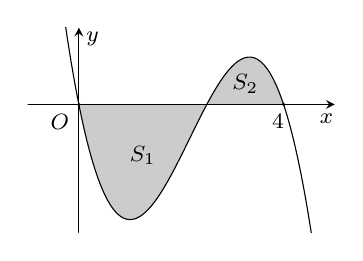
\begin{tikzpicture}[scale=0.65,>=stealth,line join=round,line cap=round,font=\footnotesize]
			\def\xmin{-1}
			\def\xmax{5}
			\def\ymin{-2.5}
			\def\ymax{1.5}
			\clip (\xmin,\ymin) rectangle (\xmax,\ymax);
			\def\f{-(\x)*(\x-2.5)*(\x-4)/2}
			\fill [gray!40] plot [domain=0:4] (\x,{\f}) -- plot[domain=4:0] (\x, {0});
			\draw [smooth, samples=100] plot [domain=\xmin:\xmax] (\x,{\f});
			\draw (1.25,-1) node {$S_1$} (3.25,.4) node {$S_2$};
			\draw [->] (\xmin,0)--(\xmax,0) node [below, xshift=-3pt] {$x$};
			\draw [->] (0,\ymin)--(0,\ymax) node [right=2pt, yshift=-4pt, fill=white, inner sep=.5pt] {$y$};
			\fill [black] (0,0) circle (1pt) node [below left] {$O$} (4,0) circle (1pt) node [below, xshift=-2pt] {$4$};
		\end{tikzpicture}
	}
	\loigiai{
		Theo đề bài, ta có $S_1=2S_2=3$ nên $S_1=3$ và $S_2=\dfrac{3}{2}$. \\
		Gọi $a$ là hoành độ giao điểm của đồ thị $y=f(x)$ và trục hoành (với $0<a<4$). \\
		Ta có  $$S_1=\displaystyle\int\limits_{0}^{a}|f(x)|\mathrm{\,d}{x}
		=-\displaystyle\int\limits_{0}^{a}f(x)\mathrm{\,d}{x} \quad (\text{vì } f(x) \le 0, \forall x \in  [0;a]).$$ \\
		Suy ra $\displaystyle\int\limits_{0}^{a}f(x)\mathrm{\,d}{x}=-3$. 
		$$S_2=\displaystyle\int\limits_{a}^{4}|f(x)|\mathrm{\,d}{x}
		=\displaystyle\int\limits_{a}^{4}f(x)\mathrm{\,d}{x} \quad (\text{vì } f(x) \ge 0, \forall x \in  [a;4]).$$ \\
		Suy ra $\displaystyle\int\limits_{a}^{4}f(x)\mathrm{\,d}{x}=\dfrac{3}{2}$. \\
		Vậy  $\displaystyle\int\limits_{0}^{4}{f(x)}\mathrm{\,d}x
		=\displaystyle\int\limits_{0}^{a}{f(x)}\mathrm{\,d}x+\displaystyle\int\limits_{a}^{4}{f(x)}\mathrm{\,d}x
		=-3+\dfrac{3}{2}=-\dfrac{3}{2}=-1{,}5$.
	}
\end{ex}
\begin{ex}%[2D4V3-1]%[Dự án đề cương 3 khối NH24-25-Dot1-Trương Tường]
	\immini{
		Hình phẳng $(H)$ tô đậm ở hình bên được giới hạn bởi đồ thị hàm số $y=\dfrac{10}{3}x-x^2$ và $y = \heva{&-x &\text{khi } x \le 1\\&x-2 &\text{khi }x > 1}$. Tính diện tích của hình $(H)$.
		\shortans[oly]{$6{,}5$}
	}
	{
		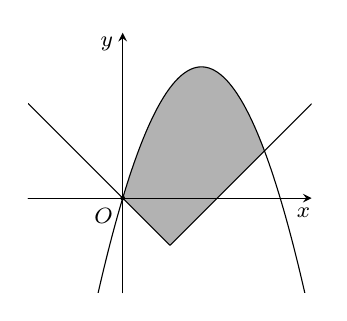
\begin{tikzpicture}[scale=0.6,>=stealth,line join=round,line cap=round,font=\footnotesize]
			% Định nghĩa khung
			\def\xmin{-2} 
			\def\xmax{4}
			\def\ymin{-2} 
			\def\ymax{3.5} 
			\def\f{10/3*(\x)-(\x)^2}
			\def\g{-\x}
			\def\h{\x-2}
			\draw [fill=gray!60,smooth,samples=100] plot [domain=0:3] (\x,{\f})--plot [domain=3:1] (\x,{\h})--plot [domain=1:0] (\x,{\g});
			\draw [->] (\xmin,0)--(\xmax,0) node [below, xshift=-3pt] {$x$};
			\draw [->] (0,\ymin)--(0,\ymax) node [left, yshift=-4pt] {$y$};
			\fill [black] (0,0) circle (0.05) node [below left] {$O$};
			\clip (\xmin,\ymin) rectangle (\xmax,\ymax);
			\draw [smooth,samples=100] plot [domain=\xmin:0] (\x,{\f}) plot [domain=3:\xmax] (\x,{\f}) plot [domain=\xmin:0] (\x,{\g}) plot [domain=3:\xmax] (\x,{\h});
		\end{tikzpicture}
	}
	\loigiai{
		Khi $x < 1$, xét phương trình $\dfrac{10}{3}x-x^2=-x \Leftrightarrow -x^2+\dfrac{13}{3}x = 0 \Leftrightarrow x=0$. \\
		Khi $x > 1$, xét phương trình $\dfrac{10}{3}x-x^2=x-2 \Leftrightarrow -x^2+\dfrac{7}{3}x+2 = 0 \Leftrightarrow x=3$. \\
		Gọi $(H_1)$ là phần hình phẳng giới hạn bởi đồ thị hai hàm số $y=\dfrac{10}{3}x-x^2$, $y=-x$ và hai đường thẳng $x=0$, $x=1$; $(H_2)$ là phần hình phẳng giới hạn bởi đồ thị hai hàm số $y=\dfrac{10}{3}x-x^2$, $y=x-2$ và hai đường thẳng $x=1$, $x=3$. \\
		Khi đó diện tích hình phẳng $(H)$ bằng tổng diện tích hai hình phẳng $(H_1)$ và $(H_2)$. \\
		Diện tích hình phẳng $(H_1)$ là $$S_1=\displaystyle\int\limits_{0}^{1}\left|\dfrac{10}{3}x-x^2-(-x)\right|\mathrm{\,d}{x}
		=\displaystyle\int\limits_{0}^{1}\left|-x^2+\dfrac{13}{3}x\right|\mathrm{\,d}{x}
		=\dfrac{11}{6}.$$
		Diện tích hình phẳng $(H_2)$ là $$S_2=\displaystyle\int\limits_{1}^{3}\left|\dfrac{10}{3}x-x^2-(x-2)\right|\mathrm{\,d}{x}
		=\displaystyle\int\limits_{1}^{3}\left|-x^2+\dfrac{7}{3}x+2\right|\mathrm{\,d}{x}
		=\dfrac{14}{3}.$$
		Vậy diện tích hình $(H)$ bằng $\dfrac{11}{6}+\dfrac{14}{3} = \dfrac{13}{2} = 6{,}5$.
	}
\end{ex}
\begin{ex}%[2D4V3-5]%[Dự án đề cương 3 khối NH24-25-Dot1-Trương Tường]
	Anh Nam dự định xây dựng một cái chòi trong sân vườn để làm nơi tụ họp gia đình. Theo tư vấn của công ty thiết kế thì để mang tính thẩm mĩ, mặt cắt qua trục của mái chòi sẽ có dạng một phần parabol $(P)$ úp ngược với chiều cao $2$ m và độ rộng của đáy bằng $4$ m (tham khảo hình bên dưới). Tính thể tích phần không gian giới hạn bởi mái chòi (kết quả làm tròn đến hàng phần mười). \\ 
	\centerline{
		\begin{tikzpicture}[scale=1,>=stealth,line join=round,line cap=round,font=\footnotesize]
			\def\g{0}
			\def\r{.85}
			\pgfmathsetmacro\ra{sqrt(1-(\r)^2)}
			\pgfmathsetmacro\a{cos(\g)}
			\pgfmathsetmacro\b{sin(\g)}
			\pgfmathsetmacro\ax{\ra*cos(\g)/sqrt((\ra*\a)^2+(\b)^2)}
			\pgfmathsetmacro\bx{\ra*sin(\g)/sqrt((\ra*\a)^2+(\b)^2)}
			\tikzset{declare function={f=2-(\x)^2/2; h=sqrt(4-(\x)^2); i=-sqrt(4-(\x)^2);}}
			\path 
			(0,0) coordinate (O)
			+({\ax},{\bx}) coordinate (i)
			+({\bx/\ra},{-\ax*\ra}) coordinate (j)
			+(0,{\r}) coordinate (k)
			;
			% Tô màu nền
			\fill [cyan!50!black!60, smooth, samples=80] plot [domain={-2}:{2}] ({\ax*\x+h*\bx/\ra}, {\bx*\x-h*\ax*\ra})--plot [domain={2}:{-2}] ({\ax*\x+i*\bx/\ra}, {\bx*\x-i*\ax*\ra})--cycle;
			%  Tô màu mái
			\fill [cyan!60, opacity=.9, smooth, samples=100] plot [domain={-2}:{2}] ({\ax*\x}, {\bx*\x+f*\r})--plot [domain={2}:{-2}] ({\ax*\x+h*\bx/\ra}, {\r*\bx*\x-h*\ax*\ra})--cycle;
			\begin{scope}
				\foreach \ga in {-180,-170,...,0}{
					\pgfmathsetmacro\A{cos(\ga)}
					\pgfmathsetmacro\B{sin(\ga)}
					\pgfmathsetmacro\Ax{\ra*cos(\ga)/sqrt((\ra*\A)^2+(\B)^2)}
					\pgfmathsetmacro\Bx{\ra*sin(\ga)/sqrt((\ra*\A)^2+(\B)^2)}
					\draw [gray, smooth, samples=80] plot [domain={0}:{2}] ({\Ax*(\x)}, {\Bx*(\x)+f*\r});
				}
			\end{scope}
			% Vẽ đường nền
			\draw [gray, smooth, samples=100, thick] plot [domain={-2}:{2}] ({\ax*\x+h*\bx/\ra}, {\bx*\x-h*\ax*\ra});
			\draw [gray, smooth, samples=100, dash pattern=on 1pt off 1pt] plot [domain={2}:{-2}] ({\ax*\x+i*\bx/\ra}, {\bx*\x-i*\ax*\ra});
			% Mặt cắt parabol
			\begin{scope}[xshift=8cm]
				\foreach \ga in {0}{
					\pgfmathsetmacro\ra{sqrt(1-(\r)^2)}
					\pgfmathsetmacro\a{cos(\ga)}
					\pgfmathsetmacro\b{sin(\ga)}
					\pgfmathsetmacro\ax{\ra*cos(\ga)/sqrt((\ra*\a)^2+(\b)^2)}
					\pgfmathsetmacro\bx{\ra*sin(\ga)/sqrt((\ra*\a)^2+(\b)^2)}
					\path 
					[samples at={-2}] plot ({\ax*\x}, {\bx*\x+f*\r}) coordinate (A)
					[samples at={2}] plot ({\ax*\x}, {\bx*\x+f*\r}) coordinate (B)
					[samples at={0}] plot ({\ax*\x}, {\bx*\x+f*\r}) coordinate (C)
					($(A)!.5!(B)$) coordinate (O')
					;
					\draw [smooth, samples=100] plot [domain={-2}:{2}] ({\ax*\x}, {\bx*\x+f*\r})--cycle;
					\draw [dash dot] ($(O')+(-90:1)$)--($(C)+(90:1)$);
					\draw [<->] ($(A)+(-90:.5)$)--($(B)+(-90:.5)$) node [midway, fill=white] {$4$};
					\draw [<->] (O')--(C) node [midway, fill=white] {$2$};
				}
			\end{scope}
		\end{tikzpicture}
	}
	\shortans[oly]{$12{,}6$}
	\loigiai{
		\immini{
			Chọn hệ trục tọa độ như hình bên. \\
			Parabol $(P)$ có đỉnh thuộc trục tung nên phương trình có dạng $y=ax^2+b$ \\
			Mà $(P)$ đi qua hai điểm $(2;0)$ và $(0;2)$ nên ta có hệ phương trình 
			$$\heva{&0 = a \cdot 2^2+b\\&2 = a \cdot 0^2+b}
			\Leftrightarrow \heva{&a = -\dfrac{1}{2}\\&b = 2.}$$
			Do đó $(P)\colon y=-\dfrac{1}{2}x^2+2$. \\
			Suy ra $x^2=4-2y$.
		}
		{
			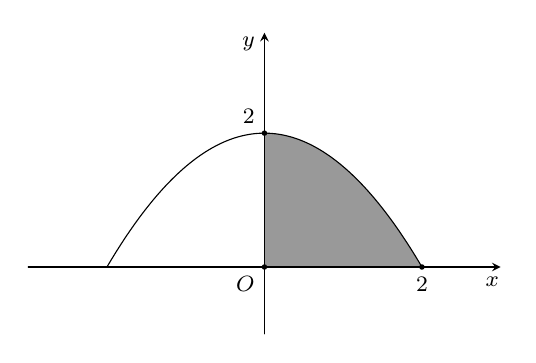
\begin{tikzpicture}[scale=1, y=.85cm, >=stealth,line join=round,line cap=round,font=\footnotesize]
				\def\xmin{-3} 
				\def\xmax{3}
				\def\ymin{-1} 
				\def\ymax{3.5} 
				\def\f{2-(\x)^2/2}
				\fill [smooth, samples=100, gray!80] plot [domain=0:2] (\x, {\f})--(0,0)--cycle;
				\draw [smooth, samples=100] plot [domain=-2:2] (\x, {\f});
				\draw [->] (\xmin,0)--(\xmax,0) node [below, xshift=-3pt] {$x$};
				\draw [->] (0,\ymin)--(0,\ymax) node [left, yshift=-4pt] {$y$};
				\fill [black] 
				(0,0) circle (1pt) node [below left] {$O$}
				(2,0) circle (1pt) node [below] {$2$}
				(0,2) circle (1pt) node [above left] {$2$};
			\end{tikzpicture}
		}
		\noindent
		Phương trình phần đồ thị $(P)$ nằm bên phải trục tung $(x \ge 0)$ là $x=\sqrt{4-2y}$. \\
		Coi phần không gian giới hạn bởi mái chòi có thể tích bằng khối tròn xoay được tạo thành khi quay quanh trục tung phần hình phẳng giới hạn bởi đồ thị $x=\sqrt{4-2y}$, trục tung và hai đường thẳng $y=0$, $y=2$. \\
		Thể tích cần tính là 
		$$V=\pi\displaystyle\int\limits_{0}^{2}\left(\sqrt{4-2y}\right)^2\mathrm{\,d}{y}
		=\pi\displaystyle\int\limits_{0}^{2}\left(4-2y\right)\mathrm{\,d}{y}
		=4\pi \approx 12{,}6 \; (\text{m}^3).$$
	}
\end{ex}
\begin{ex}%[2D4C3-5]%[Dự án đề cương 3 khối NH24-25-Dot1-Trương Tường]
	(\textit{Trích Đề thi thử tốt nghiệp THPT năm 2025 môn Toán sở GD\&ĐT Huế})
	Một lều cắm trại có dạng như hình vẽ dưới, khung lều được tạo thành từ hai parabol giống nhau có chung đỉnh $O$ và thuộc hai mặt phẳng vuông góc nhau (một parabol đi qua $A$, $O$, $C$ và một parabol đi qua $B$, $D$, $O$), bốn chân tạo thành hình vuông $ABCD$ có cạnh là $2\sqrt{2}$ m, chiều cao tính từ đỉnh lều là $2$ m. Biết mặt cắt của lều khi cắt bởi một mặt phẳng song song với mặt phẳng $(ABCD)$ luôn là một hình vuông. Tính thể tích của lều (đơn vị là $\text{m}^3$).\\ 
	\begin{minipage}{.5\textwidth}
		\centering
		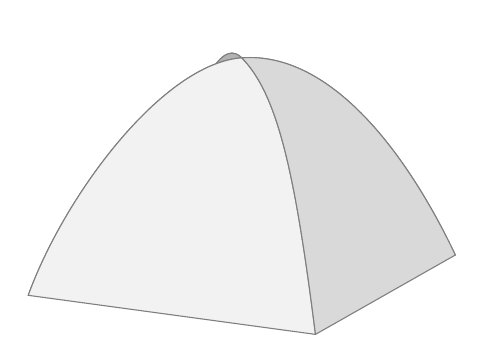
\begin{tikzpicture}[scale=.8,>=stealth,line join=round,line cap=round,font=\footnotesize]
			\path (1.17,-.94) coordinate (A)
			(3.39,.32) coordinate (B)
			(-1.17,.94) coordinate (C)
			(-3.39,-.32) coordinate (D)
			(0,3.45) coordinate (P);
			\draw [fill=gray!60,draw=gray] (B) .. controls +(-.75,1.58) and +(1.43,.1) .. (P)
			.. controls +(-.48,.47) and +(.16,1.09) .. (C)--cycle;
			\draw [fill=gray!60,draw=gray] (P) .. controls +(-.48,.47) and +(.16,1.09) .. (C)--(D)
			.. controls +(.59,1.62) and +(-1.24,-.09) .. cycle;
			\draw [fill=gray!10,draw=gray] (D) .. controls +(.59,1.62) and +(-1.24,-.09) .. (P)
			.. controls +(.58,-.59) and +(-.32,2.53) .. (A)--cycle;
			\draw [fill=gray!30,draw=gray] (P) .. controls +(.58,-.59) and +(-.32,2.53) .. (A)--(B)
			.. controls +(-.75,1.58) and +(1.43,.1) .. cycle;
		\end{tikzpicture}
	\end{minipage}
	\begin{minipage}{.5\textwidth}
		\centering
		\begin{tikzpicture}[scale=1.5,>=stealth,line join=round,line cap=round,font=\footnotesize]
			\def\g{-45}
			\def\r{.95}
			\def\xmax{3}
			\def\ymax{2}
			\def\zmax{3.5}
			\pgfmathsetmacro\ra{sqrt(1-(\r)^2)}
			\pgfmathsetmacro\a{cos(\g)}
			\pgfmathsetmacro\b{sin(\g)}
			\pgfmathsetmacro\ax{\ra*cos(\g)/sqrt((\ra*\a)^2+(\b)^2)}
			\pgfmathsetmacro\bx{\ra*sin(\g)/sqrt((\ra*\a)^2+(\b)^2)}
			\def\f{-.5*(\x)^2+2*\r}
			\path 
			(0,0) coordinate (O)
			+({\ax},{\bx}) coordinate (i)
			+({\bx/\ra},{-\ax*\ra}) coordinate (k)
			+(0,{\r}) coordinate (j)
			+($2*(j)$) coordinate (P);
			\path 
			(0,0) coordinate (O)
			[samples at={2}] plot ({\ax*\x}, {\bx*\x+\r*\f}) coordinate (A)
			[samples at={-2}] plot ({\ax*\x}, {\bx*\x+\r*\f}) coordinate (C)
			[samples at={2}] plot ({\bx/\ra*\x}, {-\ax*\ra*\x+\r*\f}) coordinate (D)
			[samples at={-2}] plot ({\bx/\ra*\x}, {-\ax*\ra*\x+\r*\f}) coordinate (B)
			;
			%
			\draw [smooth, samples=100, thick] plot [domain=-.65:2] ({\ax*\x}, {\bx*\x+\r*\f})
			plot [domain=2:-2] ({\bx/\ra*\x}, {-\ax*\ra*\x+\r*\f})
			(D)--(A)--(B);
			\draw [dash pattern=on 1pt off 2pt, samples=100] plot [domain=-.65:-2] ({\ax*\x}, {\bx*\x+\r*\f});
			\draw [dash pattern=on 1pt off 2pt] (D)--(C)--(B);
			\foreach \x/\y in {A/-90,B/0,C/180,D/180}{
				\draw [fill=black] (\x) circle (.5pt) ++(\y:0.2) node {$\x$};
			}
			\draw [fill=black] (P) circle (1pt) node [above] {$O$};
		\end{tikzpicture}
	\end{minipage}
	\shortans[oly]{$8$}
	\loigiai{
		\immini{
			Chọn mặt phẳng $Oxy$ chứa parabol $(P)$ đi qua $B$, $O$, $D$; gốc $O$ trùng với đỉnh lều, tia $Oy$ hướng xuống và chứa trục đối xứng của parabol, tia $Ox$ cùng hướng với $\vv{DB}$. \\
			Ta coi lều là phần vật thể nằm giữa hai mặt phẳng vuông góc với trục $Oy$ tại $y=0$ và $y=2$. \\
			Vì $(P)$ có đỉnh trùng gốc tọa độ $O$ nên phương trình có dạng $y=ax^2$. \\
			Có $BD=AB\sqrt{2}=4$ nên $B(2;2)$.\\
			Mà $(P)$ đi qua điểm $B(2,2)$ nên $2=a \cdot 2^2$ hay $a=\dfrac{1}{2}$. \\
			Do đó $(P)\colon y=\dfrac{1}{2}x^2$. \\
			Suy ra $x=\sqrt{2y}$ với $x \ge 0$. \\
		}
		{
			\begin{tikzpicture}[scale=1.5,>=stealth,line join=round,line cap=round,font=\footnotesize]
				\def\g{-45}
				\def\r{.95}
				\def\xmax{3}
				\def\ymax{3}
				\def\zmax{2.5}
				\pgfmathsetmacro\ra{sqrt(1-(\r)^2)}
				\pgfmathsetmacro\a{cos(\g)}
				\pgfmathsetmacro\b{sin(\g)}
				\pgfmathsetmacro\ax{\ra*cos(\g)/sqrt((\ra*\a)^2+(\b)^2)}
				\pgfmathsetmacro\bx{\ra*sin(\g)/sqrt((\ra*\a)^2+(\b)^2)}
				\def\f{-.5*(\x)^2+2*\r}
				\path 
				(0,0) coordinate (O)
				+({\ax},{\bx}) coordinate (i)
				+({\bx/\ra},{-\ax*\ra}) coordinate (k)
				+(0,{\r}) coordinate (j)
				+($2*(j)$) coordinate (P)
				%
				[samples at={2}] plot ({\ax*\x}, {\bx*\x+\r*\f}) coordinate (A)
				[samples at={-2}] plot ({\ax*\x}, {\bx*\x+\r*\f}) coordinate (C)
				[samples at={2}] plot ({\bx/\ra*\x}, {-\ax*\ra*\x+\r*\f}) coordinate (D)
				[samples at={-2}] plot ({\bx/\ra*\x}, {-\ax*\ra*\x+\r*\f}) coordinate (B)
				($(A)!.5!(C)$) coordinate (I)
				;
				%
				%					}
			\foreach \i in {1.3}{
				\fill [samples at={\i}, cyan!90!white!60] plot ({\bx/\ra*\x}, {-\ax*\ra*\x+\r*\f})--plot ({\ax*\x}, {\bx*\x+\r*\f})-- plot ({-\bx/\ra*\x}, {\ax*\ra*\x+\r*\f})
				--plot ({-\ax*\x}, {-\bx*\x+\r*\f})--cycle;
			}
			\foreach \i in {1.3}{
				\draw [samples at={\i}, gray] plot ({\bx/\ra*\x}, {-\ax*\ra*\x+\r*\f})  coordinate (D')--plot ({\ax*\x}, {\bx*\x+\r*\f})--plot ({-\bx/\ra*\x}, {\ax*\ra*\x+\r*\f}) coordinate (B');
				\draw [samples at={\i}, gray, dash pattern=on 1pt off 2pt] plot ({-\bx/\ra*\x}, {\ax*\ra*\x+\r*\f})--plot ({-\ax*\x}, {-\bx*\x+\r*\f})--plot ({\bx/\ra*\x}, {-\ax*\ra*\x+\r*\f});
				\path ($(B')!.5!(D')$) coordinate (I');
			}
			%
			\fill [cyan!90!white!60] (A)--(B)--(C)--(D)--cycle;
			\draw [smooth, samples=100, thick] 
			plot [domain=-.8:2] ({\ax*\x}, {\bx*\x+\r*\f})
			plot [domain=2:-2] ({\bx/\ra*\x}, {-\ax*\ra*\x+\r*\f})
			(D)--(A)--(B);
			\draw [dash pattern=on 1pt off 2pt, samples=100, gray] plot [domain=-.8:-2] ({\ax*\x}, {\bx*\x+\r*\f});
			\draw [dash pattern=on 1pt off 2pt, gray] (D)--(C)--(B)--cycle (A)--(C) (D')--(B')--++($(P)-(I')$) (B)--++($(P)-(I)$);
			%
			% Vẽ hệ trục
			\draw [->] ($(P)+1.25*(D)-1.25*(O)$)--($(P)+1.25*(B)-1.25*(O)$) node [above] {$x$};
			\draw [->, dash pattern=on 1pt off 2pt] (P)--++($-.8*\ymax*(j)$) node [left] {$y$};
			\draw [->] ($(P)+(C)-(O)$)--++($(A)-(C)$) node [above right] {$z$};
			\foreach \x/\y in {A/-90,B/0,C/180,D/180}{
				\draw [fill=black] (\x) circle (.5pt) ++(\y:0.2) node {$\x$};
			}
			\draw [fill=black] (P) circle (.5pt) node [above] {$O$}
			($(B')!.5!(D')$) circle (.5pt) node [above left] {$y$}
			(B')++($(P)-(I')$) circle (.5pt) node [above] {$x$}
			(I) circle (.5pt) ++(-130:.15) node {$2$}
			(B)++($(P)-(I)$) circle (.5pt) node [above] {$2$};
			\pic [draw, angle radius=0.1cm] {right angle=P--I'--D'};
			\pic [draw, angle radius=0.1cm] {right angle=P--I--D};
		\end{tikzpicture}
	}
	Như vậy, khi cắt lều bởi một mặt phẳng vuông góc với trục $Oy$ tại điểm có tung độ $y$ ta được thiết diện là hình vuông có độ dài đường chéo là $2x=2\sqrt{2y}$. \\
	Cạnh hình vuông thiết diện là $2\sqrt{y}$. \\
	Diện tích thiết diện là $S(y)=\left(2\sqrt{y}\right)^2=4y$. \\
	Thể tích chiếc lều là 
	$$V=\displaystyle\int\limits_{0}^{2}{4y}\mathrm{\,d}{y}
	= \left(2y^2\right)\Bigg|_{0}^{2}
	=8 \; \left(\text{m}^3\right).$$
}
\end{ex}
\begin{ex}%[2D4C3-5]%[Dự án đề cương 3 khối NH24-25-Dot1-Trương Tường]
\immini{
	Một cốc nước có dạng hình trụ với đường kính đáy bằng $80$ mm và chiều cao $90$ mm. Trong cốc nước có chứa một lượng nước. Đặt cốc nằm nghiêng để nước chảy ra ngoài cho đến khi mặt nước trong cốc vừa cắt ngang đáy cốc theo đường kính đáy thì dừng lại (tham khảo hình bên). Tính thể tích của lượng nước còn lại trong cốc (\textit{kết quả đơn vị ml và làm tròn đến hàng đơn vị}). 
	\shortans[oly]{$96$}
}
{
	\begin{tikzpicture}[scale=0.6, >=stealth, line join=round, font=\scriptsize]
		\path (0,0) coordinate (coc);
		% Bóng 
		\fill [gray!60] (coc)++(-.79,-1.4)++(-30:3.28)
		.. controls +(-3.7,.2) and +(-4.84,-.2) .. cycle;
		% Thân cốc
		\draw [gray,fill=gray!5] (coc)++(-.79,-1.4) coordinate (A)--++(-30:3.28) coordinate (B)
		.. controls +(.62,-.24) and +(.52,-.42) .. ++(1.61,2.79) coordinate (B') coordinate [pos=.5] (M)
		--++(150:3.28) coordinate (A') coordinate [pos=1/5] (q1) coordinate [pos=4/5] (q2) coordinate [pos=1/4] (p1) coordinate [pos=3/4] (p2)
		.. controls +(.52,-.42) and +(.62,-.24) .. ++(-1.61,-2.79);
		% Quai
		\draw [gray!70,fill=gray!60] (p1) .. controls +(1.9,.47) and +(-.54,1.88) .. (p2)--(q2)
		.. controls +(-.07,2.05) and +(1.81,.96) .. (q1);
		\path ($(A)!.5!(A')$) coordinate (O)
		($(B)!.5!(B')$) coordinate (O')
		($2*(O')-(M)$) coordinate (N)
		;
		% Nước
		\begin{scope}
			\clip (M)--(N)--(A)--++(-30:3.8);
			\fill [gray!40] (coc)++(-.79,-1.4)++(-30:3.28)
			.. controls +(.62,-.24) and +(.52,-.42) .. ++(1.61,2.79)
			.. controls +(-.52,.42) and +(-.62,.24) .. ++(-1.61,-2.79);
		\end{scope}
		\fill [gray!40] (A)--(B)--(O');
		\fill [gray!60] (coc)++(-.79,-1.4) .. controls +(.29,-.25) and +(-.8,-.12) .. (M)--(N)
		.. controls +(-.8,.2) and +(.95,.1) .. cycle;
		\draw [gray!80] (A) .. controls +(-.62,.24) and +(-.52,.42) .. ++(1.61,2.79)
		.. controls +(.52,-.42) and +(.62,-.24) .. ++(-1.61,-2.79);
		\draw [dashed,dash pattern=on 1pt off 1pt,gray] (B) .. controls +(-.62,.24) and +(-.52,.42) .. ++(1.61,2.79)
		(B)--(B') (A)--(O') (M)--(N);	
		\draw [|<->|] (B)++(-30:1)--++($(B')-(B)$) node [midway,sloped,fill=white,inner sep=1pt] {$80$ mm};
		\draw [|<->|] (B')++(60:2)--++($(A)-(B)$) node [midway,sloped,fill=white,inner sep=1pt] {$90$ mm};
	\end{tikzpicture}
}
\loigiai{
	\immini{
		Chọn hệ trục tọa độ $Oxyz$ như hình bên. \\
		Coi phần nước còn lại trong cốc như phần vật thể nằm giữa hai mặt phẳng $x=-40$ và $x=40$.\\
		Cắt phần nước theo một mặt phẳng vuông góc với trục $Ox$ ta điểm có hoành độ $x$ $(-40 \le x \le 40)$ ta được thiết diện là tam giác $HKL$ vuông tại $K$.\\
		Ta có 
		\begin{itemize}
			\item $KL=\sqrt{OK^2-OL^2} = \sqrt{40^2 - x^2} = \sqrt{1\,600-x^2}$.
			\item $\widehat{AOB}=\widehat{HLK}$ (góc tạo bởi mặt nước và mặt đáy cốc).
			\item $HK = KL\cdot \tan\widehat{HLK} = KL\cdot\tan \widehat{AOB} = \sqrt{1\;600-x^2}\cdot \dfrac{90}{40} = \dfrac{9\sqrt{1\;600-x^2}}{4}$.
		\end{itemize}
		Diện tích tam giác $HKL$ là
		$$S(x)=\dfrac{1}{2}\cdot HK\cdot KL = \dfrac{9}{8}\left(1\;600-x^2\right) = 1\,800 - \dfrac{9}{8}x^2.$$
		Thể tích phần nước còn lại trong cốc là 
		$$V=\displaystyle\int_{-40}^{40}{\left(1\,800 - \dfrac{9}{8}x^2\right)}\mathrm{\,d}x = 96\,000 \; \left(\text{mm}^3\right) \approx 96 \text{ (ml).}$$ 
	}{
		\begin{tikzpicture}[scale=0.7, >=stealth, line join=round, font=\scriptsize]
			\path (0,0) coordinate (coc) coordinate (O);
			\begin{scope}[rotate=-60]
				% Thân cốc
				\draw [gray,fill=gray!5] (coc)++(-.79,-1.4) coordinate (A)--++(-30:3.28) coordinate (B)
				.. controls +(.62,-.24) and +(.52,-.42) .. ++(1.61,2.79) coordinate (B') coordinate [pos=.18] (K) coordinate [pos=.45] (M)
				--++(150:3.28) coordinate (A') coordinate [pos=1/5] (q1) coordinate [pos=4/5] (q2) coordinate [pos=1/4] (p1) coordinate [pos=3/4] (p2)
				.. controls +(.52,-.42) and +(.62,-.24) .. ++(-1.61,-2.79);
				% Quai
				\draw [gray!70,fill=gray!60] (p1) .. controls +(1.9,.47) and +(-.54,1.88) .. (p2)--(q2)
				.. controls +(-.07,2.05) and +(1.81,.96) .. (q1);
				%
				\path
				(A)++(0:{3.28/cos(30)}) coordinate (I)
				++($(A)-(B)$) coordinate (I')
				($(B)!.5!(B')$) coordinate (O')
				(B)++(180:{3.28*cos(30)}) coordinate (B1)
				(B) .. controls +(-.62,.24) and +(-.52,.42) .. ++(1.61,2.79) coordinate [pos=.55] (N)
				;
				\path [name path=l] (coc)++(-.79,-1.4) .. controls +(.29,-.25) and +(-.8,-.12) .. (M);
				\path [name path=h] (K)--++($(A)-(B)$) coordinate (h);
				\path [name intersections={of=l and h, by={H}}];
				\path (intersection cs: first line={(K)--($(K)+(B')-(B)$)}, second line={(M)--(N)}) coordinate (L);
				% Nước
				\begin{scope}
					\clip (M)--(N)--(A)--++(-30:3.8);
					\fill [gray!40] (B)
					.. controls +(.62,-.24) and +(.52,-.42) .. ++(1.61,2.79)
					.. controls +(-.52,.42) and +(-.62,.24) .. ++(-1.61,-2.79);
				\end{scope}
				\fill [gray!40] (A)--(B)--(O');
				\fill [gray!60] (A) .. controls +(.29,-.25) and +(-.8,-.12) .. (M)--(N)
				.. controls +(-.8,.1) and +(.95,.2) .. cycle;
				\draw [gray!80] (A) .. controls +(-.62,.24) and +(-.52,.42) .. ++(1.61,2.79)
				.. controls +(.52,-.42) and +(.62,-.24) .. ++(-1.61,-2.79);
				\draw [dashed,dash pattern=on 1pt off 1pt,gray] (B) .. controls +(-.62,.24) and +(-.52,.42) .. ++(1.61,2.79)
				(B)--(B') (A)--(O') (M)--(N);
				\foreach \x in {A,B,M,N,H,K,L,O'}{
					\fill[gray] (\x) circle (1pt);
				}
				\draw [gray] (H)--(K);
				\draw [dashed,dash pattern=on 1pt off 1pt,gray] (H)--(L)--(K) (O)--(O') (N)--++($(N)-(O')$);
				\fill [pattern=north east lines, pattern color=gray]  (H)--(K)--(L); 
				\draw [->,gray] (O)--++(150:1.5) node [left] {$z$};
				\draw [->,gray] (M)--++($(M)-(N)$) node [below] {$x$};
				\draw [->,gray] (B)--++($.5*(B)-.5*(I)$) node [below] {$y$};
				;
				\draw (O') node [xshift=7pt,yshift=4pt]{$O$} (L) node [xshift=4pt,yshift=-2.5pt] {$x$} (M) node [xshift=4pt,yshift=-4pt] {$40$} (N) node [xshift=10pt,yshift=3pt] {$-40$}
				(H) node [yshift=4pt]{$H$} (K) node [xshift=-4pt,yshift=-4pt]{$K$} (L) node [xshift=5pt,yshift=2.5pt]{$L$} 
				;
			\end{scope}
			\fill (-1.5,-3.35) node[above left]{$B$};
			\fill (-1.5,0) node[left]{$A$};
		\end{tikzpicture}
	}
}
\end{ex}
\Closesolutionfile{ans}
%\indapan{6}{ans/2D4-Bai3-TLN}

\ind{PHẦN IV.} \inden{Tự luận.}\\
\setcounter{ex}{0}
\begin{ex}%[2D4N3-1]%[Dự án đề cương 3 khối NH24-25-Dot1-Trương Tường]
(\textit{Trích đề thi HKII - Trường THPT Nguyễn Gia  Thiều - Hà Nội}) \\
Tính diện  tích hình phẳng giới hạn bởi đồ thị hàm số $y=\cos{x}$, trục hoành, trục tung và đường thẳng $x=\dfrac{\pi}{6}$.
\loigiai{
	Ta có $\cos{x}>0$, $\forall x \in \left[0;\dfrac{\pi}{6}\right]$.\\
	Do đó, diện tích cần tính là 
	$$ V = \displaystyle\int\limits_{0}^{\tfrac{\pi}{6}}\cos{x}\mathrm{\,d}{x} = \displaystyle\int\limits_{0}^{\tfrac{\pi}{6}}\cos{x}\mathrm{\,d}{x} = \left(\sin{x}\right)\Bigg|_{0}^{\tfrac{\pi}{6}} = \sin{\dfrac{\pi}{6}}-\sin{0} = \dfrac{1}{2}. $$
}
\end{ex}
\begin{ex}%[2D4H3-1]%[Dự án đề cương 3 khối NH24-25-Dot1-Trương Tường]
Tính diện tích phần hình phẳng giới hạn bởi đồ thị hai hàm số $y=2x^3-x$, $y=x$ và hai đường thẳng $x=-1$, $x=1$. 
\loigiai{
	Diện tích cần tìm là $$S=\displaystyle\int\limits_{-1}^{1}\left|2x^3-x-x\right|\mathrm{\,d}{x}
	=\displaystyle\int\limits_{-1}^{1}\left|2x^3-2x\right|\mathrm{\,d}{x}$$
	Xét phương trình $2x^3-2x=0 \Leftrightarrow 2x(x^2-1)=0 \Leftrightarrow \hoac{&x=0\\&x=\pm 1.}$ \\
	Do đó 
	\allowdisplaybreaks
	\begin{eqnarray*}
		&S&=\displaystyle\int\limits_{-1}^{0}\left|2x^3-2x\right|\mathrm{\,d}{x}+\displaystyle\int\limits_{0}^{1}\left|2x^3-2x\right|\mathrm{\,d}{x} \\
		&&=\displaystyle\int\limits_{-1}^{0}\left(2x^3-2x\right)\mathrm{\,d}{x}+\displaystyle\int\limits_{0}^{1}\left(2x-2x^3\right)\mathrm{\,d}{x} \quad (\text{vì } 2x^3-2x \ge 0, \forall x \in [-1;0] \text{ và } 2x^3-2x \le 0, \forall x \in [0;1])  \\
		&&= \left(\dfrac{x^4}{2}-x^2\right)\Bigg|_{-1}^{0} + \left(x^2-\dfrac{x^4}{2}\right)\Bigg|_{0}^{1} \\
		&&=-\left(\dfrac{1}{2}-1\right)+\left(1-\dfrac{1}{2}\right) \\
		&&=1.
	\end{eqnarray*}
}
\end{ex}
\begin{ex}%[2D4H3-3]%[Dự án đề cương 3 khối NH24-25-Dot1-Trương Tường]
Biết thể tích khối tròn xoay tạo nên khi quay xung quanh trục $Ox$ hình phẳng giới hạn bởi các đường $y=(1-x)^2$, $y=0$, $x=0$, $x=2$ có dạng $\dfrac{a\pi}{b}$ với $\dfrac{a}{b}$ là phân số tối giản. Tính giá trị biểu thức $S=24a+12b$. \\
\centerline{
	\begin{tikzpicture}[scale=1.5,>=stealth,line join=round,line cap=round,font=\footnotesize]
		%% Xây dựng hệ tọa độ Oxyz
		\def\g{-1}
		\def\r{.996}
		\pgfmathsetmacro\ra{sqrt(1-(\r)^2)}
		\pgfmathsetmacro\a{cos(\g)}
		\pgfmathsetmacro\b{sin(\g)}
		\pgfmathsetmacro\ax{\ra*cos(\g)/sqrt((\ra*\a)^2+(\b)^2)}
		\pgfmathsetmacro\bx{\ra*sin(\g)/sqrt((\ra*\a)^2+(\b)^2)}
		% Định nghĩa giá trị min -max trên trục tọa độ
		\def\xmax{3}
		\def\ymax{1.5}
		\def\zmax{7}
		\def\m{0}
		\def\n{2}
		% Định nghĩa các hàm số 
		\pgfmathdeclarefunction{h}{1}{%
			\pgfmathparse{(1-#1)^2} 
		}
		% Định nghĩa vectơ đơn vị và các điểm khác
		\path 
		(0,0) coordinate (O)
		+({\ax},{\bx}) coordinate (i)
		+({\bx/\ra},{-\ax*\ra}) coordinate (k)
		+(0,{\r}) coordinate (j)
		;
		% Vẽ
		\fill [orange!60!black!80, smooth, samples=80,opacity=.5] plot [domain={\m}:{\n}] ({\ax*\x}, {h(\x)*\r+\x*\bx})
		--($\n*(i)$)--($\m*(i)$)--cycle
		;
		\begin{scope}
			\pgfmathsetmacro{\Rn}{h(\n)}
			\pgfmathsetmacro{\Rm}{h(\m)}
			\def\i{sqrt((\Rn)^2-(\x)^2)}
			\def\j{sqrt((\Rm)^2-(\x)^2)}
			\fill [cyan, smooth, samples=80, opacity=.6] plot [domain={0}:{\Rn}] ({\x*\bx/\ra+\n*\ax}, {\n*\bx-\x*\ax*\ra+\i*\r})
			--plot [domain={\Rn}:{0}] ({\x*\bx/\ra+\n*\ax}, {\n*\bx-\x*\ax*\ra-\i*\r})
			--plot [domain={\n}:{\m}] ({\ax*\x}, {-h(\x)*\r+\x*\bx})
			--plot [domain={0}:{\Rm}] ({\x*\bx/\ra+\m*\ax}, {\m*\bx-\x*\ax*\ra-\j*\r})
			--plot [domain={\Rm}:{0}] ({\x*\bx/\ra+\m*\ax}, {\m*\bx-\x*\ax*\ra+\j*\r})
			--plot [domain={\m}:{\n}] ({\ax*\x}, {h(\x)*\r+\x*\bx})--cycle
			;
			\fill [cyan!60, smooth, samples=80, opacity=.5] plot [domain={0}:{-\Rn}] ({\x*\bx/\ra+\n*\ax}, {\n*\bx-\x*\ax*\ra+\i*\r})
			--plot [domain={-\Rn}:{0}] ({\x*\bx/\ra+\n*\ax}, {\n*\bx-\x*\ax*\ra-\i*\r})
			--plot [domain={\n}:{\m}] ({\ax*\x}, {-h(\x)*\r+\x*\bx})
			--plot [domain={0}:{-\Rm}] ({\x*\bx/\ra+\m*\ax}, {\m*\bx-\x*\ax*\ra-\j*\r})
			--plot [domain={-\Rm}:{0}] ({\x*\bx/\ra+\m*\ax}, {\m*\bx-\x*\ax*\ra+\j*\r})
			--plot [domain={\m}:{\n}] ({\ax*\x}, {h(\x)*\r+\x*\bx})--cycle
			;
			\draw [smooth, samples=80, opacity=.5] 
			plot [domain={-\Rn}:{\Rn}] ({\x*\bx/\ra+\n*\ax}, {\n*\bx-\x*\ax*\ra+\i*\r})
			--plot [domain={\Rn}:{-\Rn}] ({\x*\bx/\ra+\n*\ax}, {\n*\bx-\x*\ax*\ra-\i*\r})--cycle
			plot [domain={0}:{\Rm}] ({\x*\bx/\ra+\m*\ax}, {\m*\bx-\x*\ax*\ra-\j*\r}) coordinate (t)
			--plot [domain={\Rm}:{0}] ({\x*\bx/\ra+\m*\ax}, {\m*\bx-\x*\ax*\ra+\j*\r})
			;
			\draw [smooth, samples=80, opacity=.5, dash pattern=on 1pt off 1pt] 
			plot [domain={0}:{-\Rm}] ({\x*\bx/\ra+\m*\ax}, {\m*\bx-\x*\ax*\ra-\j*\r})
			--plot [domain={-\Rm}:{0}] ({\x*\bx/\ra+\m*\ax}, {\m*\bx-\x*\ax*\ra+\j*\r})
			;
		\end{scope}
		\begin{scope}
			\foreach \k in {.5,1,2,4}{
				\pgfmathsetmacro\t{sqrt(1+(\k)^2)}
				\draw [smooth, samples=80, very thin, gray] plot [domain={\m}:{\n}] ({\ax*\x+\k*h(\x)/\t*\bx/\ra}, {h(\x)/\t*\r+\x*\bx-\k*h(\x)/\t*\ax*\ra})
				;
				\draw [smooth, samples=80, very thin, gray] plot [domain={\m}:{\n}] ({\ax*\x+\k*h(\x)/\t*\bx/\ra}, {-h(\x)/\t*\r+\x*\bx-\k*h(\x)/\t*\ax*\ra})
				;
			}
		\end{scope}
		\draw [smooth, samples=80, very thin, gray] plot [domain={\m}:{\n}] ({\ax*\x+h(\x)*\bx/\ra}, {\bx*\x-h(\x)*\ax*\ra})
		;
		%	
		\draw [smooth, samples=80, gray] plot [domain={\n}:{\m}] ({\ax*\x}, {-h(\x)*\r+\x*\bx})
		plot [domain={\n}:{\m}] ({\ax*\x}, {h(\x)*\r+\x*\bx});
		% Vẽ hệ trục
		\draw [gray] ($\n*(i)$)--({\n*\ax},{\n*\bx+h(\n)*\r});
		\draw [dash pattern=on 1pt off 1pt, gray] ($\m*(i)$)--({\m*\ax},{\m*\bx+h(\m)*\r});
		\draw [->] ($\n*(i)$)--($\xmax*(i)$) node [right] {$x$};
		\draw (O)--($\m*(i)$);
		\draw [dash pattern=on 1pt off 1pt, gray] ($\m*(i)$)--($\n*(i)$);
		\draw [->] (O)--($\zmax*(k)$) node [left] {$z$};
		\draw [->] (O)--($\ymax*(j)$) node [left] {$y$};
		\fill (O) circle (1pt) node [above left] {$O$};
		%\draw [thick] (O) circle (\R);
	\end{tikzpicture}
}
\loigiai{
	Thể tích khối tròn xoay là 
	$$V=\pi\displaystyle\int\limits_{0}^{2}{(1-x)^4}\mathrm{\,d}{x}
	=\dfrac{2\pi}{5}.$$
	Do đó $a=2$ và $b=5$. \\
	Vậy $24a+12b=24 \cdot 2+12 \cdot 5=108$.
}
\end{ex}
\begin{ex}%[2D4H3-1]%[Dự án đề cương 3 khối NH24-25-Dot1-Trương Tường]
\immini{
	Cho hai hàm số $y=\dfrac{x^3}{4}$ và $y=x$ có đồ thị như hình bên. Tính diện tích phần đồ thị được tô đậm.
}
{
	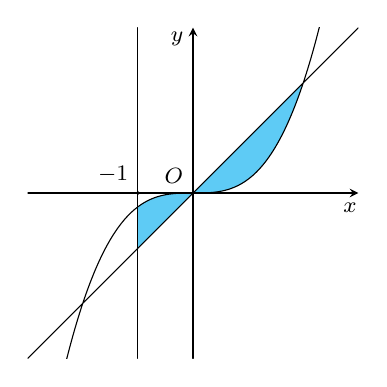
\begin{tikzpicture}[scale=0.7,>=stealth,line join=round,line cap=round,font=\footnotesize]
		\def\xmin{-3} 
		\def\xmax{3}
		\def\ymin{-3} 
		\def\ymax{3} 
		\clip (\xmin,\ymin) rectangle (\xmax,\ymax);
		\def\f{(\x)^3/4}
		\def\g{\x}
		%
		\fill [cyan!90!white!70, smooth, samples=100] plot [domain=-1:2] (\x, {\f})--plot [domain=2:-1] (\x, {\g})--cycle;
		\draw [smooth, samples=100] plot [domain=\xmin:\xmax] (\x, {\f})
		plot [domain=\xmin:\xmax] (\x, {\g});
		\draw (-1,\ymin)--(-1,\ymax);
		%
		\draw [->] (\xmin,0)--(\xmax,0) node [below, xshift=-3pt] {$x$};
		\draw [->] (0,\ymin)--(0,\ymax) node [left, yshift=-4pt] {$y$};
		\fill [black] (0,0) circle (1pt) node [above left] {$O$}
		(-1,0) circle (1pt) node [above left] {$-1$};
	\end{tikzpicture}
}
\loigiai{
	Xét phương trình $\dfrac{x^3}{4}=x \Leftrightarrow \hoac{&x=0\\&x=\pm 2.}$ \\
	Phần tô đậm là hình phẳng giới hạn bởi đồ thị hàm số $y=\dfrac{x^3}{4}$, $y=x$ và hai đường thẳng $x=-1$, $x=2$ nên có diện tích 
	\allowdisplaybreaks
	\begin{eqnarray*}
		&S&=\displaystyle\int\limits_{-1}^{2}\left|\dfrac{x^3}{4}-x\right|\mathrm{\,d}{x} \\
		&&=\displaystyle\int\limits_{-1}^{0}\left|\dfrac{x^3}{4}-x\right|\mathrm{\,d}{x}+\displaystyle\int\limits_{0}^{2}\left|\dfrac{x^3}{4}-x\right|\mathrm{\,d}{x} \\
		&&=\displaystyle\int\limits_{-1}^{0}\left(\dfrac{x^3}{4}-x\right)\mathrm{\,d}{x} + \displaystyle\int\limits_{0}^{2}\left(x-\dfrac{x^3}{4}\right)\mathrm{\,d}{x} \\
		&&= \left(\dfrac{x^4}{16}-\dfrac{x^2}{2}\right)\Bigg|_{-1}^{0} + \left(\dfrac{x^2}{2}-\dfrac{x^4}{16}\right)\Bigg|_{0}^{2} \\
		&&=-\left[\dfrac{(-1)^3}{16}-\dfrac{(-1)^2}{2}\right]+\left(\dfrac{2^2}{2}-\dfrac{2^4}{16}\right) \\
		&&=\dfrac{7}{16}+1 \\
		&&=\dfrac{23}{16}.
	\end{eqnarray*}
}
\end{ex}
\begin{ex}%[2D4H3-1]%[Dự án đề cương 3 khối NH24-25-Dot1-Trương Tường]
(\textit{Trích đề thi HKII - Sở GD\&ĐT Bình Dương - Năm học 2024-2025}) \\
Một cánh buồm được mô tả như hình vẽ bên dưới. Tính diện tích cánh buồm. \\
\centerline{
	\begin{tikzpicture}[scale=0.5,>=stealth,line join=round,line cap=round,font=\footnotesize]
		\def\xmin{-1} 
		\def\xmax{4}
		\def\ymin{-1} 
		\def\ymax{9} 
		\clip (\xmin,\ymin) rectangle (\xmax,\ymax);
		\def\f{2^(\x)}
		\fill [smooth, samples=100,  pattern=north west lines] plot [domain=1:3] (\x, {\f})--(3,2)--cycle;
		\draw [smooth, samples=100, thick] plot [domain=\xmin:\xmax] (\x, {\f});
		%
		\draw [dash pattern=on 1pt off 2pt] (1,0)--(1,2)--(0,2) (3,0)--(3,8)--(0,8)
		(1,2)--(3,2);
		\draw [thick]  (1,2)--(3,2)--(3,8);
		\draw [->] (\xmin,0)--(\xmax,0) node [below, xshift=-3pt] {$x$};
		\draw [->] (0,\ymin)--(0,\ymax) node [left, yshift=-4pt] {$y$};
		\draw [fill=black] (0,0) circle (1pt) node [below left] {$O$}
		(1,0) circle (1pt) node [below] {$1$}
		(3,0) circle (1pt) node [below] {$3$}
		(0,2) circle (1pt) node [left] {$2$}
		(0,8) circle (1pt) node [left] {$8$}
		(1,2) circle (1pt) (3,8) circle (1pt) (3,2) circle (1pt);
		
	\end{tikzpicture}
}
\loigiai{
	Phần cánh buồn là  hình phẳng giới hạn bởi đồ thị hai hàm số $y=2^x$, $y=2$ và hai đường thẳng $x=1$, $x=3$ nên có diện tích
	\allowdisplaybreaks 
	\begin{eqnarray*}
		&S&=\displaystyle\int\limits_{1}^{3}\left|2^{x}-2\right|\mathrm{\,d}{x} \\
		&&=\displaystyle\int\limits_{1}^{3}\left(2^{x}-2\right)\mathrm{\,d}{x} \quad (\text{vì } 2^x \ge  2, \; \forall x \in  [1;3]) \\
		&&= \left(\dfrac{2^x}{\ln{2}}-2x\right)\Bigg|_{1}^{3} \\
		&&=\left(\dfrac{2^3}{\ln2}-2 \cdot 3\right)-\left(\dfrac{2^1}{\ln{2}}-2 \cdot 1\right) \\
		&&=\dfrac{6}{\ln{2}}-4.
	\end{eqnarray*}
}
\end{ex}
\begin{ex}%[2D4H3-4]%[Dự án đề cương 3 khối NH24-25-Dot1-Trương Tường]
(\textit{Trích đề HKII - Trường THPT Nguyễn Tất Thành – TP.HCM - Năm học 2024-2025}) \\
Tính thể tích $V$ của vật thể nằm giữa hai mặt phẳng $x=0$ và $x=\pi$, biết thiết diện của vật thể bị cắt bởi một mặt phẳng vuông góc với trục $Ox$ tại điểm có hoành độ $x$ ($0 \leq x \leq \pi$) là tam giác đều cạnh là $2\sqrt{\sin x}$.
\loigiai{
	Thiết diện là tam giác đều cạnh  $2\sqrt{\sin x}$ nên có diện tích $$S(x)=\left(2\sqrt{\sin x}\right)^2 \cdot \dfrac{\sqrt{3}}{4}=\sqrt{3} \cdot \sin x.$$
	Thể tích $V$ cần tính là 
	$$V=\displaystyle\int\limits_{0}^{\pi}\sqrt{3} \cdot \sin x\mathrm{\,d}{x}
	= \left(-\sqrt{3} \cdot \cos x\right)\Bigg|_{0}^{\pi}
	= -\sqrt{3}\cdot\cos\pi + \sqrt{3}\cdot\cos 0
	= 2\sqrt{3}.$$
}
\end{ex}
\begin{ex}%[2D4V3-5]%[Dự án đề cương 3 khối NH24-25-Dot1-Trương Tường]
\immini{
	Một nhà máy dự định sản suất các viên gạch men lát sàn cao cấp, mỗi viên có dạng hình vuông cạnh $80$ cm. Theo qui trình sản suất, mỗi viên gạch sẽ trải qua ba công đoạn liên tiếp: công đoạn tạo hình với chi phí $60\,000$ đồng/$\text{m}^2$, công đoạn tráng men toàn bộ viên gạch với chi phí $10\,000$ đồng/$\text{m}^2$ và công đoạn trang trí. Trong công đoạn trang trí, người ta in màu xám $4$ góc và một hình tròn ngay tâm của viên gạch. Biết rằng nếu đặt viên gạch trong một hệ trục tọa độ $Oxy$ sao cho gốc $O$ trùng với tâm viên gạch (đơn vị mỗi trục là $10$ cm) thì một đỉnh viên gạch có tọa độ $(4;4)$ và phần in màu xám ở góc chứa đỉnh này giới hạn bởi đồ thị hàm số $y=\dfrac{4}{x}$ và hai cạnh của viên gạch (phần in màu ở $4$ góc có diện tích bằng nhau); phần in màu ở tâm là hình tròn bán kính $\sqrt{2}$ (tham khảo hình bên). Chi phí in màu xám là $7\,000$ đồng/$\text{m}^2$.
}
{
	
\begin{tikzpicture}[scale=0.6,>=stealth,line join=round,line cap=round,font=\footnotesize]
		\def\a{4}
		\def\f{\a/(\x)}
		\def\g{-\a/(\x)}
		\path (0,0) coordinate (O)
		+(\a,\a) coordinate (A)
		+(-\a,\a) coordinate (B)
		+(-\a,-\a) coordinate (C)
		+(\a,-\a) coordinate (D);
		\draw [fill=gray!5] (A)--(B)--(C)--(D)--cycle;
		\fill [gray] (O) circle ({sqrt(2)});
		\foreach \g in {0,90,180,270}{
			\fill [gray, smooth, samples=100, rotate=\g] plot [domain=1:4] (\x, {\f})--(\a,\a)--cycle;
		}
		
	\end{tikzpicture}
}
\noindent
Mỗi viên gạch sẽ được bán với giá $85\,000$ đồng. Hỏi nếu nhà máy bán được $5\,000$ viên gạch thì lợi nhuận thu được là bao nhiêu triệu đồng (\textit{kết quả làm tròn đến hàng đơn vị})?
\loigiai{
	Diện tích của mỗi viên gạch là $S=0{,8}^2=0{,}64$ $\left(\text{m}^2\right)$. \\
	Diện tích phần hình tròn là $S_{1}=\pi \cdot \left(0{,}1\sqrt{2}\right)^2 \approx 0{,}063$ $\left(\text{m}^2\right)$. \\
	Xét phần in màu xám giới hạn bởi đồ thị hàm số $y=\dfrac{4}{x}$ và hai cạnh viên gạch: \\
	Phương trình hai cạnh của viên gạch lần lượt là $x=4$ và $y=4$. \\
	Phương trình $\dfrac{4}{x}=4$ có nghiệm $x=1$. \\
	Do đó phần hình phẳng này giới hạn bởi hai đồ thị hàm số $y=\dfrac{4}{x}$, $y=4$ và hai đường thẳng $x=1$, $x=4$. \\
	Diện tích phần hình phẳng này là \[S_{2}=0{,}1^2 \cdot \displaystyle\int\limits_{1}^{4}{\left(4-\dfrac{4}{x}\right)\mathrm{\,d}{x}}
	\approx 0{,}0645 \; \left(\text{m}^2\right).\]
	Diện tích các phần in màu là $S'=S_{1}+4S_{2}=0{,}321$ $\left(\text{m}^2\right)$.\\
	Chi phí sản suất mỗi viên gạch là 
	$70\,000 \cdot 0{,}64+7\,000 \cdot 0{,}321=47\,047$ (đồng).
	\\
	Lợi nhuận thu được khi bán mỗi viên gạch là $85\,000-47\,047=37\,953$ (đồng).\\
	Vậy lợi nhuận thu được khi bán $5\,000$ viên gạch là $5\,000 \cdot 37\,953 \approx 190$ (triệu đồng). 
}
\end{ex}
\begin{ex}%[2D4V3-5]%[Dự án đề cương 3 khối NH24-25-Dot1-Trương Tường]
(\textit{Trích đề KSCL học kỳ II Toán 12 năm 2024 – 2025 sở GD\&ĐT Nam Định})  \\
Một chậu cây có chiều cao là $30$ cm và đường kính miệng chậu là $30$ cm. Mặt cắt ngang của chậu cây là một đường parabol (tham khảo hình vẽ). \\
\begin{minipage}{.5\textwidth}
	\centering
	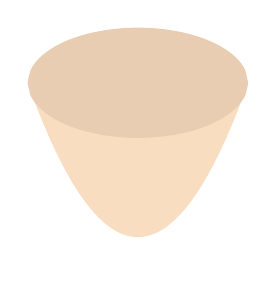
\begin{tikzpicture}[scale=.7,>=stealth,line join=round,line cap=round,font=\footnotesize]
		\def\g{0}
		\def\r{.7}
		\def\xmax{10}
		\def\ymax{5}
		\def\zmax{5}
		\pgfmathsetmacro\ra{sqrt(1-(\r)^2)}
		\pgfmathsetmacro\a{cos(\g)}
		\pgfmathsetmacro\b{sin(\g)}
		\pgfmathsetmacro\ax{\ra*cos(\g)/sqrt((\ra*\a)^2+(\b)^2)}
		\pgfmathsetmacro\bx{\ra*sin(\g)/sqrt((\ra*\a)^2+(\b)^2)}
		\def\h{sqrt(4-(\x)^2)}
		\def\i{-sqrt(4-(\x)^2)}
		\def\f{(\x)^2}
		\path 
		(0,0) coordinate (O)
		+({\ax},{\bx}) coordinate (i)
		+({\bx/\ra},{-\ax*\ra}) coordinate (j)
		+(0,{\r}) coordinate (k)
		;
		\fill [orange!90!black!30, opacity=.8, smooth, samples=100] plot [domain={-2}:{2}] ({\ax*\x}, {\bx*\x+(\f)*\r})--cycle;
		\fill [orange!70!black!30, smooth, samples=80] plot [domain={-2}:{2}] ({\ax*\x+\h*\bx/\ra}, {\r*\bx*\x-\r*\h*\ax*\ra+4*\r})--plot [domain={2}:{-2}] ({\ax*\x+\i*\bx/\ra}, {\r*\bx*\x-\r*\i*\ax*\ra+4*\r})--cycle;	
	\end{tikzpicture}
\end{minipage}
\begin{minipage}{.5\textwidth}
	\centering
	\begin{tikzpicture}[scale=.7,>=stealth,line join=round,line cap=round,font=\footnotesize]
		\def\g{0}
		\def\r{.7}
		\def\xmax{10}
		\def\ymax{5}
		\def\zmax{5}
		\pgfmathsetmacro\ra{sqrt(1-(\r)^2)}
		\pgfmathsetmacro\a{cos(\g)}
		\pgfmathsetmacro\b{sin(\g)}
		\pgfmathsetmacro\ax{\ra*cos(\g)/sqrt((\ra*\a)^2+(\b)^2)}
		\pgfmathsetmacro\bx{\ra*sin(\g)/sqrt((\ra*\a)^2+(\b)^2)}
		\def\h{sqrt(4-(\x)^2)}
		\def\i{-sqrt(4-(\x)^2)}
		\def\f{(\x)^2}
		\path 
		(0,0) coordinate (O)
		+({\ax},{\bx}) coordinate (i)
		+({\bx/\ra},{-\ax*\ra}) coordinate (j)
		+(0,{\r}) coordinate (k)
		plot [samples at={-2}] ({\ax*\x}, {\bx*\x+(\f)*\r}) coordinate (B)
		plot  [samples at={2}] ({\ax*\x}, {\bx*\x+(\f)*\r}) coordinate (A)
		;
		\draw [smooth, samples=100] plot [domain={-2}:{2}] ({\ax*\x}, {\bx*\x+(\f)*\r})--cycle;
		\draw [<->] (A)--(B) node [midway, fill=white] {$30$};
		\draw [<->] (A)--++($-4*(k)$) node [midway, right] {$30$};
		\draw [dash pattern=on 1pt off 2pt] (O)--++($2*(i)$);
		\draw [dash dot] (0,-1)--(0,4);
	\end{tikzpicture}
\end{minipage}
Tính thể tích của chậu cây đó (đơn vị: $\mathrm{dm}^3$). (\textit{Kết quả làm tròn đến hàng phần mười}).
\loigiai{
	\immini{
		Chọn hệ trục tọa độ $Oxy$ sao cho gốc tọa độ $O$ trùng với đỉnh của parabol $(P)$, trục $Oy$ chứa trục đối xứng của parabol như hình vẽ. \\
		Gọi $(H)$ là phần hình phẳng giới hạn bởi phần đồ thị $(P)$ nằm bên phải trục tung, trục tung và hai đường thẳng $y=0$, $y=30$. \\
		Coi chậu cây là vật thể được tạo thành khi quay $(H)$ quanh trục tung. \\
		Phương trình $(P)$ có dạng $y=ax^2$. \\
		Mà $(P)$ đi qua điểm $(15;30)$ nên $30=a \cdot 15^2$ hay $a=\dfrac{2}{15}$. \\
		Do đó $(P):y=\dfrac{2}{15}x^2$.
	}
	{
		\begin{tikzpicture}[scale=.7,>=stealth,line join=round,line cap=round,font=\footnotesize]
			\def\g{0}
			\def\r{.7}
			\def\xmax{10}
			\def\ymax{5}
			\def\zmax{5}
			\pgfmathsetmacro\ra{sqrt(1-(\r)^2)}
			\pgfmathsetmacro\a{cos(\g)}
			\pgfmathsetmacro\b{sin(\g)}
			\pgfmathsetmacro\ax{\ra*cos(\g)/sqrt((\ra*\a)^2+(\b)^2)}
			\pgfmathsetmacro\bx{\ra*sin(\g)/sqrt((\ra*\a)^2+(\b)^2)}
			\def\h{sqrt(4-(\x)^2)}
			\def\i{-sqrt(4-(\x)^2)}
			\def\f{(\x)^2}
			\path 
			(0,0) coordinate (O)
			+({\ax},{\bx}) coordinate (i)
			+({\bx/\ra},{-\ax*\ra}) coordinate (j)
			+(0,{\r}) coordinate (k)
			;
			\draw [smooth, samples=100] plot [domain={-2}:{2}] ({\ax*\x}, {\bx*\x+(\f)*\r})--cycle;
			\draw [dash pattern=on 1pt off 2pt] ($2*(i)$)--++($4*(k)$)--++($-4*(i)$)--++($-4*(k)$);
			\draw [->] (O)--($5.5*(k)$) node [left, yshift=-3pt] {$y$};
			\draw [->] ($-3*(i)$)--($3*(i)$) node [below, xshift=-3pt] {$x$};
			\draw [fill=black] (O) circle (1pt) node [below] {$O$}
			($2*(i)$) circle (1pt) node [below] {$15$}
			($-2*(i)$) circle (1pt) node [below] {$-15$}
			($4*(k)$) circle (1pt) node [above left] {$30$};
		\end{tikzpicture}
	}
	\noindent
	Suy ra phần đồ thị nằm bên phải trục tung là $x=\sqrt{\dfrac{15y}{2}}$.\\
	Thể tích chậu cây là 
	$$V=\pi\displaystyle\int\limits_{0}^{30}\left(\sqrt{\dfrac{15y}{2}}\right)^2\mathrm{\,d}{y}
	=\pi\displaystyle\int\limits_{0}^{30}\dfrac{15y}{2}\mathrm{\,d}{y}
	=\pi\left.\left(\dfrac{15y^2}{4}\right)\right|_{0}^{30}
	=3\,375\pi \; \left(\text{cm}^3\right) 
	\approx 10{,}6 \; \left(\text{dm}^3\right).$$ 
}
\end{ex}
\begin{ex}%[2D4C3-5]%[Dự án đề cương 3 khối NH24-25-Dot1-Trương Tường]
\immini{
	Sân nhà của anh Hùng có dạng hình chữ nhật với kích thước $8 \text{ m} \times 6 \text{m}$. Chọn hệ trục tọa độ $Oxy$ sao cho gốc $O$ trùng với tâm của sân, hai trục $Ox$ và $Oy$ lần lượt song song với hai cạnh sân. Anh Hùng sử dụng đồ thị $(C)$ của hàm số $y=\dfrac{ax^2+b}{x}$ $(a, \; b \in \mathbb{R})$ để chia sân thành ba phần: phần thứ nhất giới hạn bởi $(C)$ và hai cạnh sân, phần thứ hai giới hạn bởi $(C)$ và hai cạnh sân ở góc sân đối diện phần thứ nhất, phần thứ ba là phần còn lại của sân. Anh Hùng dự định làm một hồ cá ở phần thứ nhất, trồng hoa ở phần thứ hai, lát đá làm lối đi ở phần thứ ba và phần rộng nhất của lối đi là $5$ m (tham khảo hình bên).\\
	Anh Hùng được đơn vị thi công tư vấn rằng chi phí làm hồ cá là $200\,000$ đồng/$\text{m}^2$; chi phí trồng hoa là $100\,000$ đồng/$\text{m}^2$ và chi phí lát đá là $250\,000$ đồng/$\text{m}^2$. Hỏi theo dự định thì chi phí anh Hùng bỏ ra để trang trí sân nhà là bao nhiêu triệu đồng? (\textit{Kết quả làm tròn đến hàng phần mười}).
}
{
	\begin{tikzpicture}[scale=0.5,>=stealth,line join=round,line cap=round,font=\footnotesize]
		\def\xmin{-5.5} 
		\def\xmax{5.5}
		\def\ymin{-5} 
		\def\ymax{5} 
		\clip (\xmin,\ymin) rectangle (\xmax,\ymax);
		\def\f{((\x)^2-4)/(\x)}
		\fill [pattern=bricks, pattern color=gray, smooth, samples=100]  plot [domain=-4:-1] (\x, {\f})-- plot [domain=4:1] (\x, {\f})--cycle;
		\fill [pattern=crosshatch dots gray, pattern color=gray, smooth, samples=100] plot [domain=-4:-1] (\x, {\f})--(-4,3)--cycle;
		\fill [pattern=sixpointed stars, pattern color=gray, smooth, samples=100] plot [domain=4:1] (\x, {\f})--(4,-3)--cycle;
		\draw [smooth, samples=100] plot [domain=-4:-1] (\x, {\f})
		plot [domain=1:4] (\x, {\f});
		\draw [thick] (-4,-3) rectangle (4,3);
		\draw [->] (\xmin,0)--(\xmax,0) node [below, xshift=-3pt] {$x$};
		\draw [->] (0,\ymin)--(0,\ymax) node [left, yshift=-4pt] {$y$};
		\fill [black] (0,0) circle (1pt) node [fill=white] {$O$};
		\draw [|<->|] (-4,-3.5)--(1,-3.5) node [midway, fill=white, inner sep=0pt] {$5$ m};
		\draw [|<->|] (-4.5,-3)--(-4.5,3) node [midway, sloped, fill=white, inner sep=0pt] {$6$ m};
		\draw [|<->|] (-4,3.5)--(4,3.5) node [midway, fill=white, inner sep=0pt] {$8$ m};
		\draw [dash pattern=on 1pt off 1pt] (-4,-3)--++(-90:.5) (1,-3)--++(-90:.5) (-4,-3)--++(180:.5) (-4,3)--++(180:.5) (-4,3)--++(90:.5) (4,3)--++(90:.5);
	\end{tikzpicture}
}

\loigiai{
	Đồ thị $(C)$ đi qua hai điểm $(1;-3)$ và $(4;3)$ nên ta có hệ phương trình 
	$$\heva{&\dfrac{a+b}{1} = -3\\&\dfrac{16a+b}{4} = 3}
	\Leftrightarrow  \heva{&a+b = -3\\&16a+b = 12}
	\Leftrightarrow \heva{&a = 1\\&b = -4.} $$
	Suy ra $(C)\colon y=\dfrac{x^2-4}{x}$. \\
	Do tính đối xứng của đồ thị $(C)$ nên phần thứ nhất và phần thứ hai có diện tích bằng nhau. \\
	Phần thứ nhất giới hạn bởi hai đồ thị hàm số: $y=\dfrac{x^2-4}{x}$, $y=-3$ và hai đường thẳng $x=1$ và $x=4$ nên có diện tích 
	\[S_1=\displaystyle\int\limits_{1}^{4}\left(\dfrac{x^2-4}{x}+3\right)\mathrm{\,d}{x} = \dfrac{15}{2} - 8\ln 2 \approx 10{,}96 \; \left(\text{m}^2\right).\]
	Diện tích phần thứ ba là $S_3 = 8 \cdot 6 - 2 \cdot 10{,}96=26{,}08 \; \left(\text{m}^2\right)$.\\
	Chi phí anh Hùng dự định bỏ ra là 
	\[10{,}96 \cdot 200+10{,}96 \cdot 100+26{,}08 \cdot 250=9\,808 \; \text{(nghìn đồng)} \approx 9{,}8 \; \text{(triệu đồng)}.\]
}
\end{ex}
\begin{ex}%[2D4C3-5]%[Dự án đề cương 3 khối NH24-25-Dot1-Trương Tường]
(\textit{Trích đề HKII - Trường Nguyễn Bỉnh Khiêm – Hà Nội - Năm học 2024-2025})
\immini{
	Một viên gạch hình vuông có cạnh bằng $40$ cm. Người ta dùng bốn đường parabol có chung đỉnh tại tâm của viên gạch để tạo ra bốn cánh hoa (được tô màu như hình vẽ). Hỏi diện tích phần cánh hoa được tô màu của viên gạch bằng bao nhiêu centimet vuông \textit{(kết quả làm tròn đến hàng đơn vị)}?
}
{
	\begin{tikzpicture}[scale=0.7,>=stealth,line join=round,line cap=round,font=\footnotesize]
		\def\f{(\x)^2/2}
		\foreach \x in {0,1,2,3}{
			\draw [fill=gray!45,rotate=\x*90,smooth,samples=100]
			plot[domain=0:2](\x, {\f})
			--plot[domain=2:0] ({\f},\x)--cycle;
		}
		\draw (-2,-2) rectangle (2,2);
	\end{tikzpicture}
}
\loigiai{
	\immini{
		Chọn hệ trục tọa độ $Oxy$ sao cho $O$ trùng với tâm hình vuông, tia $Ox$, $Oy$ vuông góc với các cạnh hình vuông như hình bên. \\
		Xét một cánh hoa nằm ở góc phần tư thứ nhất. \\
		Cánh hoa này là phần hình phẳng giới hạn bởi hai parabol $(P_1)\colon y=ax^2$ và $(P_2)\colon x=by^2$ (với $y \ge 0$).\\
		Vì $(P_1)$ và $(P_2)$ đi qua điểm $(20;20)$ nên 
		$$\heva{&20 =a \cdot 20^2\\&20 =b \cdot 20^2}
		\Leftrightarrow
		\heva{&a =\dfrac{1}{20}\\&b = \dfrac{1}{20}.}$$
		Như vậy $(P_1)\colon y=\dfrac{x^2}{20}$ và $(P_2)\colon x=\dfrac{y^2}{20}$. \\
		Phần đồ thị $(P_2)$ nằm phía trên trục hoành có phương trình $y=\sqrt{20x}$.\\
		Diện tích của một cánh hoa là 
		\allowdisplaybreaks
		\begin{eqnarray*}
			&S&=\displaystyle\int\limits_{0}^{20}\left|\sqrt{20x}-\dfrac{x^2}{20}\right|\mathrm{\,d}{x}\\
			&&=\displaystyle\int\limits_{0}^{20}\left(\sqrt{20x}-\dfrac{x^2}{20}\right)\mathrm{\,d}{x} \quad (\text{vì } \sqrt{20x} \ge \dfrac{x^2}{20},\; \forall x \in [0;20]) \\
			&&=\left.\left(\sqrt{20}\cdot \dfrac{2}{3} \cdot \sqrt{x^3}-\dfrac{x^3}{60}\right)\right|_{0}^{20}  \\
			&&=\dfrac{400}{3} \text{ (cm).}
		\end{eqnarray*}
	}
	{
		\begin{tikzpicture}[scale=0.7,>=stealth,line join=round,line cap=round,font=\footnotesize]
			\def\xmin{-3} 
			\def\xmax{3}
			\def\ymin{-3} 
			\def\ymax{3} 
			\def\f{(\x)^2/2}
			\foreach \x in {1,2,3}{
				\draw [fill=gray!45,rotate=\x*90,smooth,samples=100]
				plot[domain=0:2](\x, {\f})
				--plot[domain=2:0] ({\f},\x)--cycle;
			}
			\draw [pattern=north west lines,smooth,samples=100]
			plot[domain=0:2](\x, {\f})
			--plot[domain=2:0] ({\f},\x)--cycle;
			\draw (-2,-2) rectangle (2,2);
			\draw [->] (\xmin,0)--(\xmax,0) node [below, xshift=-3pt] {$x$};
			\draw [->] (0,\ymin)--(0,\ymax) node [left, yshift=-4pt] {$y$};
			\fill [black] (0,0) circle (1pt) node [below left] {$O$}
			(2,0) circle  (1pt) node [below right] {$20$}
			(0,2) circle (1pt) node [above left] {$20$};
		\end{tikzpicture}
	}
}
\end{ex}

\indapan{10}{ans/2D4-Bai3-TN}
\indapan{4}{ans/2D4-Bai3-DS}
\indapan{6}{ans/2D4-Bai3-TLN}